\documentclass[12pt,twoside,notitlepage]{report}

% Some texcount commands so that we count text that occurs in tables
%TC:group table 0 1
%TC:group tabular 1 1
%TC:group tabularx 2 1
%TC:group lstlisting 0 1

%packages
\usepackage{float}                  % Allow use of H for figures, to allow for exact placement
\usepackage{a4}
\usepackage{hyperref}
\usepackage{verbatim}
\usepackage{booktabs, longtable}
\usepackage{tabularx}
\usepackage{xcolor,colortbl}
\usepackage{hhline}
\usepackage{graphicx}
\usepackage{subcaption}
\usepackage{epstopdf}
\usepackage{listings}       % Source code listings
\usepackage[toc]{glossaries}
\usepackage{changebar}
\usepackage{amsmath}
\usepackage{amssymb}
\usepackage{rotating}
\usepackage{tikz}
\usepackage{pgfplots}
\usepackage{pgfplotstable}
\usepackage[utf8]{inputenc}
\usepackage{graphicx}
\usepackage{framed}                 % Frames/boxes - used in appendix describing file formats
\usepackage{enumitem}               % Fancier item lists - used for lists in languages and tools section
\usepackage{hyperref}               % Reference urls
\usepackage{tabularx}               % Allows the width of a tabular environment to be specified along with the use of X in the collumn specifiers
\usepackage{mathtools}
\usepackage{hyperref}
\usepackage[bottom]{footmisc}

% Shorthands
% Var in mathmode
\newcommand{\var}{\text{Var}}
% vectors in mathmode
\newcommand{\vc}[1]{\mathbf{#1}}
% math fonts shorthand
\newcommand{\cl}[1]{\mathcal{#1}}
\newcommand{\bb}[1]{\mathbb{#1}}
%Argmin/max operators
\DeclareMathOperator*{\argmin}{arg\,min}
\DeclareMathOperator*{\argmax}{arg\,max}
% Maximum likelihood and maximum a-posterior
\newcommand{\ML}{\text{ML}}
\newcommand{\MAP}{\text{MAP}}

% Names for the datasets we have
\newcommand{\siris}{the BSS }
\newcommand{\tengs}{[[Teng's]]}

% Def eq math symbol
\newcommand\defeq{\stackrel{\mathclap{\normalfont\tiny\mbox{def}}}{=}}

% Numbering on subsubsections
\setcounter{secnumdepth}{3}

% Tikz imports
\usetikzlibrary{
    arrows,
    shapes,
    snakes,
    automata,
    backgrounds,
    calc,
    petri,
    patterns,
    shapes.misc,
    patterns,
    matrix,
    chains,
    positioning,
    decorations.pathreplacing,
    arrows,
}

% Tikz styles
\pgfplotsset{soldot/.style={color=blue,only marks,mark=*}} 
\pgfplotsset{holdot/.style={color=blue,fill=white,only marks,mark=*}}

%Setup listings env for when we don't want to use minted
\lstset{
  basicstyle=\footnotesize\tt,                                          % the size of the fonts that are used for the code
  breakatwhitespace=false,                                              % sets if automatic breaks should only happen at whitespace
  breaklines=true,                                                      % sets automatic line breaking
  prebreak = \raisebox{0ex}[0ex][0ex]{\ensuremath{\hookleftarrow}},     % add arrows to indicate line breaks added
  framesep = 5px,                                                       % add padding to the top/bottom of listings
  captionpos=b,                                                          % sets the caption-position to bottom
  extendedchars=true,                                                   % lets you use non-ASCII characters; for 8-bits encodings only, does not work with UTF-8
  frame=single,                                                             % adds a frame around the code (frame at bot and top)
  language=Java,                                                        % the language of the code
  showspaces=false,                                                     % show spaces everywhere adding particular underscores; it overrides 'showstringspaces'
  showstringspaces=false,                                               % underline spaces within strings only
  showtabs=false,                                                       % show tabs within strings adding particular underscores
  tabsize=4,                                                            % sets default tabsize to 4 spaces
  numbers=left,                                                         % puts numbers on the left side
  keywordstyle=\color[rgb]{0,0,1}\ttfamily,
  stringstyle=\color[rgb]{0.627,0.126,0.941}\ttfamily,
  commentstyle=\color[rgb]{0.133,0.545,0.133}\ttfamily,
  morecomment=[l][\color{magenta}]{\#},
  aboveskip=2em,                                                        % spacing above listings
  belowskip=1.5em,                                                         % spacing below listings
}

% Graphics extensions used
\DeclareGraphicsExtensions{.pdf, .svg, .png, .jpg, .jpeg, .eps}
\graphicspath{ {figs/} }

% ??
\newcolumntype{R}{>{\raggedleft\arraybackslash}X}

% Pick the bibliocraphy style
\bibliographystyle{plain}

% Styling for pgf plots
\pgfplotsset{compat=newest}
\pgfplotsset{grid style={gray!50}}
\pgfplotsset{minor grid style={dashed,gray!50}}

%colours for bar graphs
\pgfplotsset{
   /pgfplots/bar  cycle  list/.style={/pgfplots/cycle  list={%
        {blue,fill=blue!50!white,mark=none},%
        {orange,fill=orange!50!white,mark=none},%
        {green,fill=green!50!white,mark=none},%
        {yellow,fill=yellow!40!white,mark=none},%
        {red,fill=red!50!white,mark=none},%
     }
   },
}

\usepgfplotslibrary{units}

% to allow postscript inclusions
\input{epsf}                 
% On thor and CUS read top of file:
%     /opt/TeX/lib/texmf/tex/dvips/epsf.sty
% On CL machines read:
%     /usr/lib/tex/macros/dvips/epsf.tex

% glossaries
\makeglossaries

\raggedbottom                           % try to avoid widows and orphans
\sloppy
\clubpenalty1000%
\widowpenalty1000%

\addtolength{\oddsidemargin}{6mm}       % adjust margins
\addtolength{\evensidemargin}{-8mm}

\renewcommand{\baselinestretch}{1.1}    % adjust line spacing to make
                                        % more readable

\begin{document}


% glossary definitions
% \newacronym{btb}{BTB} {Branch Target Buffer}
% \newacronym{bp0}{BTB8} {branch predictor with BTB and tablesize 8}
% \newacronym{bp1}{BTB512} {branch predictor with BTB and tablesize 512}
% \newacronym{sat}{SAT} {branch predictor with 3-bit saturating counters}
% \newacronym{lhbp}{LHBP} {local history branch predictor}
% \newacronym{pc}{PC} {Program Counter}
% \newacronym{alu}{ALU} {Arithmetic Logic Unit}
% \newacronym{risc}{RISC} {Reduced Instruction Set Computer}
% \newacronym{ISA}{ISA} {Instruction Set Architecture}
% \newacronym{ipc}{IPC} {Instructions Per Cycle}
% \newacronym{cpi}{CPI} {Cycles per Instruction}
% \newacronym{fpga}{FPGA} {Field Programmable Logic Array}
% \newacronym{alut}{ALUT}{Adaptive Look-Up Table}
% \newacronym{alm}{ALM} {Adaptive Logic Module}

%%%%%%%%%%%%%%%%%%%%%%%%%%%%%%%%%%%%%%%%%%%%%%%%%%%%%%%%%%%%%%%%%%%%%%%%%%%%%%%%%%%%%%%%%%%%%%%%%%%%%%%%%%%%%%%%%%%%%%%%
% Title

% Remove page numbering for title page
\pagenumbering{gobble}

% Name
\begin{flushright}
    \Large
    \hfill{\LARGE \bf Michael Painter}
\end{flushright}

% Title + imgs
\begin{center}
    \vfill

    \Huge{\bf Spectral Image Analysis for Medical Imaging}
    
    \bigskip
    \bigskip
    
    {Part II Computer Science Tripos} \\
    
    \bigskip
    
    {Churchill College, 2016\\}

    \bigskip 

    {\today}

    \bigskip

    
\includegraphics[scale=0.099]{titleimg/camcrest}
    
\includegraphics[scale=0.2792]{titleimg/chucrest}

    \vfill
\end{center}





%%%%%%%%%%%%%%%%%%%%%%%%%%%%%%%%%%%%%%%%%%%%%%%%%%%%%%%%%%%%%%%%%%%%%%%%%%%%%%%%%%%%%%%%%%%%%%%%%%%%%%%%%%%%%%%%%%%%%%%%
% Proforma

\cleardoublepage

\setcounter{page}{1}
\pagenumbering{roman}
\pagestyle{plain}

\chapter*{Proforma}

{\large
\begin{tabularx}{\textwidth}{l X}
Name:               & \bf Michael Painter                      \\
College:            & \bf Churchill College                     \\
Project Title:      & \bf Spectral Image Analysis for Medical Imaging \\
Examination:        & \bf Computer Science Part II Project Dissertation, May 2016        \\
Word Count:         & \bf 8432\footnotemark[1]\\
Project Originator: & Dr Pietro Lio'              \\
Supervisor:         & Dr Pietro Lio' \& Dr Gianluca Ascolani       \\ 
\end{tabularx}
}

\footnotetext[1]{
    This word count was computed by {\tt texcount.pl -total diss.tex }
}
\stepcounter{footnote}


\section*{Original aims of the project}
    *TODO*

\section*{Work completed}
    *TODO*

\section*{Special difficulties}
    None.
 




%%%%%%%%%%%%%%%%%%%%%%%%%%%%%%%%%%%%%%%%%%%%%%%%%%%%%%%%%%%%%%%%%%%%%%%%%%%%%%%%%%%%%%%%%%%%%%%%%%%%%%%%%%%%%%%%%%%%%%%%
% Declaration

\cleardoublepage
\section*{Declaration}

I, Michael Painter of Churchill College, being a candidate for Part II of the Computer Science Tripos, hereby declare 
that this dissertation and the work described in it are my own work, unaided except as may be specified below, and that 
the dissertation does not contain material that has already been used to any substantial extent for a comparable 
purpose.

\bigskip
\bigskip
\bigskip
\bigskip

\leftline{\rule{6cm}{0.5pt}}
\leftline{Signed}

\bigskip
\bigskip
\bigskip
\bigskip

\leftline{\rule{4cm}{0.5pt}}
\leftline{Date}










%%%%%%%%%%%%%%%%%%%%%%%%%%%%%%%%%%%%%%%%%%%%%%%%%%%%%%%%%%%%%%%%%%%%%%%%%%%%%%%%%%%%%%%%%%%%%%%%%%%%%%%%%%%%%%%%%%%%%%%%
% the contents

\cleardoublepage
\setcounter{tocdepth}{1}
\tableofcontents










%%%%%%%%%%%%%%%%%%%%%%%%%%%%%%%%%%%%%%%%%%%%%%%%%%%%%%%%%%%%%%%%%%%%%%%%%%%%%%%%%%%%%%%%%%%%%%%%%%%%%%%%%%%%%%%%%%%%%%%%
% list of figures, tables and listings

\listoffigures

\listoftables

\lstlistoflistings










%%%%%%%%%%%%%%%%%%%%%%%%%%%%%%%%%%%%%%%%%%%%%%%%%%%%%%%%%%%%%%%%%%%%%%%%%%%%%%%%%%%%%%%%%%%%%%%%%%%%%%%%%%%%%%%%%%%%%%%%
% acknowledgements

\clearpage
\section*{Acknowledgements}

I thank my supervisors, director of studies and tutor for their extensive support, especially for putting up with me 
throughout the year. I would like to thank Malavika Nair, Ioana Bica and Clare Pacini for diligently proofreading 
this dissertation when it was abruptly thrust into their hands and also for their general support, helping me keep 
it together through the tougher parts of the year. Further thanks to are definitely due to Yanie de Nadaillac for 
basically being my general life coach.










%%%%%%%%%%%%%%%%%%%%%%%%%%%%%%%%%%%%%%%%%%%%%%%%%%%%%%%%%%%%%%%%%%%%%%%
% now for the chapters

\cleardoublepage        % just to make sure before the page numbering
                        % is changed

\setcounter{page}{1}
\pagenumbering{arabic}
\pagestyle{headings}















%%%%%%%%%%%%%%%%%%%%%%%%%%%%%%%%%%%%%%%%%%%%%%%%%%%%%%%%%%%%%%%%%%%%%%%%%%%%%%%%%%%%%%%%%%%%%%%%%%%%%%%%%%%%%%%%%%%%%%%%
% the introduction

\cleardoublepage
\chapter{Introduction}
    In this chapter we introduce the problem: what sort of data are we given and what would we like to do with it? We 
    begin by introducing new terminology, and specifically by defining terms that might otherwise be ambiguous. We briefly 
    discuss the motivation behind the implementation of this system, then suggest some possible methods that 
    could be used to implement a solution. We decide on one solution to explore and identify what we might hope to discover 
    by exploring said solution.

    \section{Terminology and preliminary definitions} \label{sec:term_and_def}
        It is sensible to start by introducing some terminology and preliminary definitions, as they will be used frequently throughout the 
        dissertation, including even the rest of the introduction chapter.

        Firstly let $\bb{N}_k$ where $k\in \bb{N}$ denote the set $\{ n \in \bb{N}\ |\ n < k \} = 
        \{0, 1, ..., (k-1)\}$. And let $\bb{B}$ denote the set $\{0, 1\} = \bb{N}_2$, which will be used for boolean choices.

        Typically, the word \textit{spectral} refers to use of the Fourier domain; for example 
        \textit{spectral methods} refers to the use of Fourier domain to solve differential equations. For our 
        purposes the \textit{spectrum} of some signal is the Fourier transform of the time-domain signal and more 
        specifically, referring to a quantised spectrum. The word \textit{spectrum} refers to 
        either a continuous or quantised spectrum, for which the context should make it obvious which one is 
        intended. 

        \begin{figure}
            \centering

                \scalebox{0.80}{ 
                    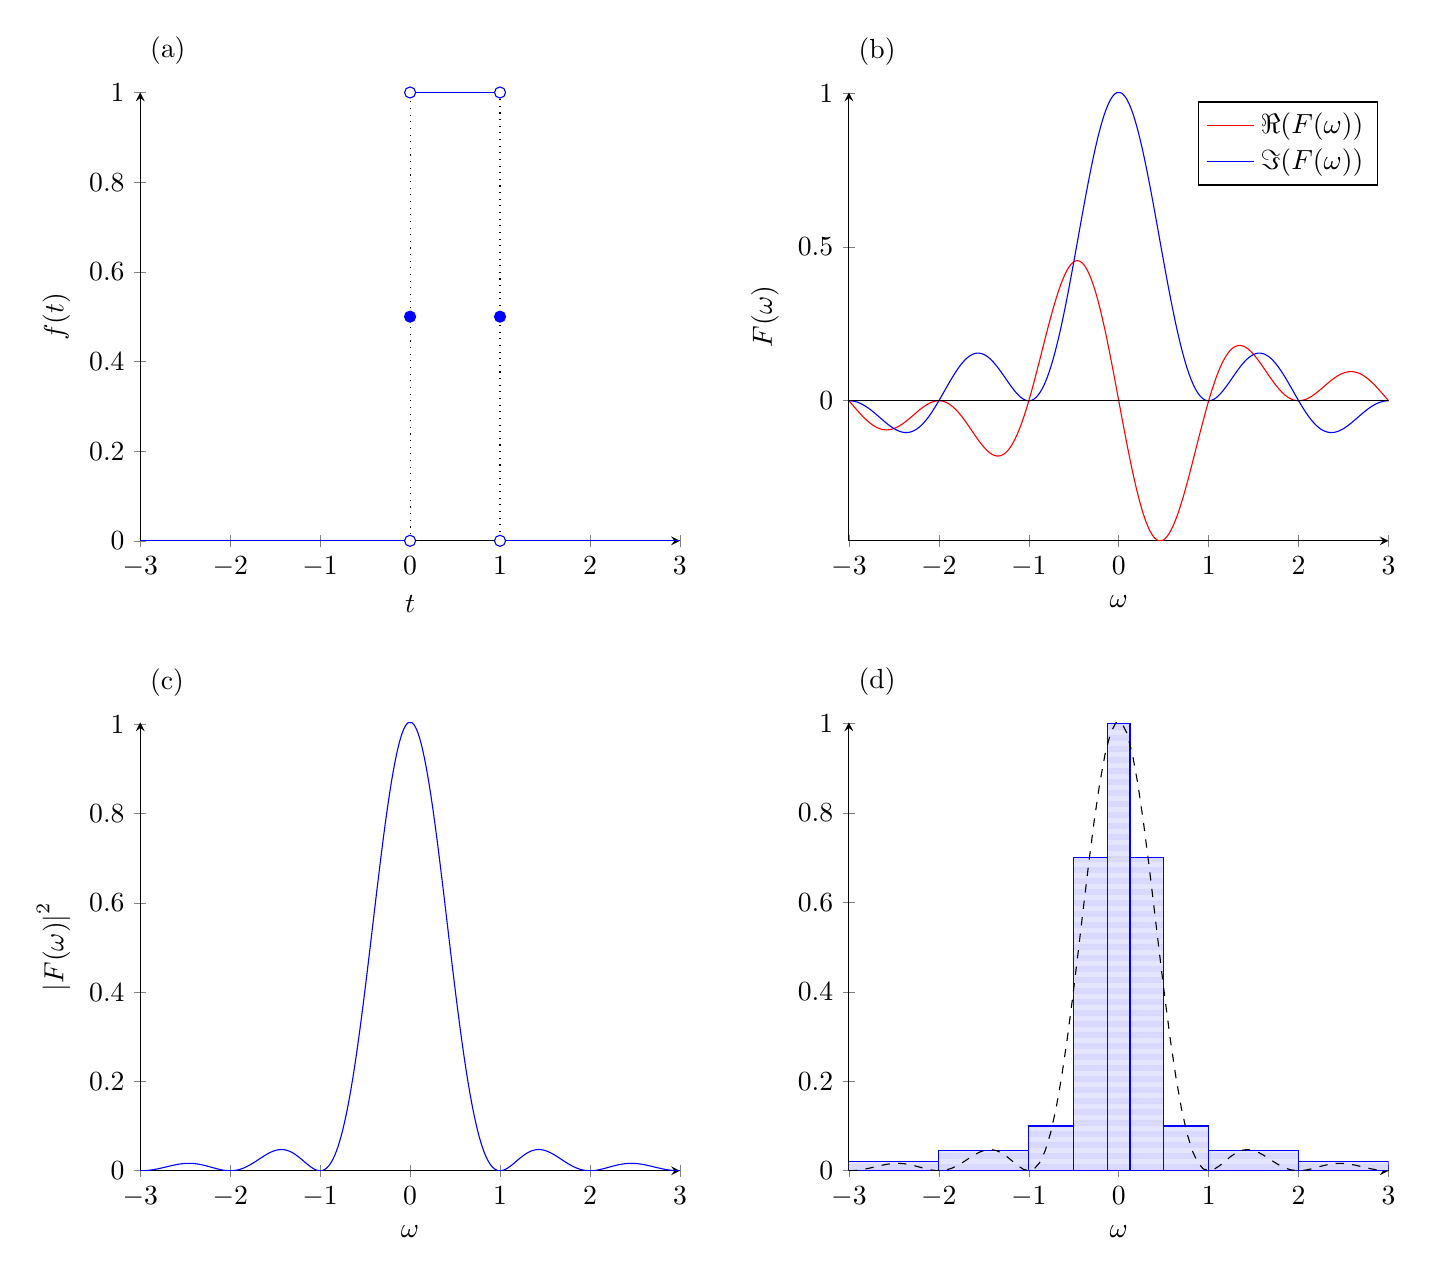
\begin{tikzpicture}
                        \begin{scope}
                            \begin{axis}[
                                name = plot1,
                                axis lines = left,
                                xlabel = $t$,
                                ylabel = $f(t)$
                            ]
                                \addplot[domain=-3:0, blue] {0};
                                \addplot[domain=0:1, blue] {1};
                                \addplot[domain=1:3, blue] {0};
                                \draw[dotted] (axis cs:0,0) -- (axis cs:0,1);
                                \draw[dotted] (axis cs:1,1) -- (axis cs:1,0);
                                \addplot[holdot] coordinates{(0,0)(0,1)(1,1)(1,0)};
                                \addplot[soldot] coordinates{(0,0.5)(1,0.5)};
                            \end{axis}
                            \node at (plot1.above north west) [anchor=south west] {(a)};
                        \end{scope}

                        \begin{scope}[xshift=9cm]
                            \begin{axis}[
                                name = plot2,
                                axis lines = left,
                                xlabel = $\omega$,
                                ylabel = $F(\omega)$
                            ]
                                \addplot[domain=-3:3, samples = 500, red] {((sin(deg(x) * pi))/((deg(x) * pi) * 1.74 * 0.01)) * sin(-(deg(x)*pi)/2)};
                                \addlegendentry{$\Re(F(\omega))$}
                                \addplot[domain=-3:3, samples = 500, blue] {((sin(deg(x) * pi))/((deg(x) * pi) * 1.74 * 0.01)) * cos(-(deg(x)*pi)/2)};
                                \addlegendentry{$\Im(F(\omega))$}
                                \draw (axis cs:-3,0) -- (axis cs:3,0);
                            \end{axis}
                            \node at (plot2.above north west) [anchor=south west] {(b)};
                        \end{scope}

                        \begin{scope}[yshift=-8cm]
                            \begin{axis}[
                                name = plot3,
                                axis lines = left,
                                xlabel = $\omega$,
                                ylabel = $\left|F(\omega)\right|^2$
                            ]
                                \addplot[domain=-3:3, samples = 500, blue] {((sin(deg(x) * pi))/((deg(x) * pi) * 1.74 * 0.01))^2};
                            \end{axis}
                            \node at (plot3.above north west) [anchor=south west] {(c)};
                        \end{scope}

                        \begin{scope}[xshift=9cm, yshift=-8cm]
                            \begin{axis}[
                                name = plot4,
                                axis lines = left,
                                xlabel = $\omega$,
                            ]
                                \addplot[ybar interval, draw=blue,pattern=horizontal lines light blue] coordinates {
                                    (-3,0.02) 
                                    (-2,0.045)
                                    (-1,0.1)
                                    (-0.5,0.7)
                                    (-0.125,1)
                                    (0.125,0.7)
                                    (0.5,0.1)
                                    (1,0.045)
                                    (2,0.02)
                                    (3,0.02)
                                };
                                \addplot[domain=-3:3, samples = 100, dashed] {((sin(deg(x) * pi)/((deg(x) * pi) * 1.74 * 0.01))^2};
                            \end{axis}
                            \node at (plot4.above north west) [anchor=south west] {(d)};
                        \end{scope}


                    \end{tikzpicture}
                }


            \caption{Examples of (a) a time-domain signal $f(t)$, (b) it's Fourier transform $F(\omega)$, (c) it's power 
                spectrum $|F(\omega)|^2$ and (d) a quantisation of c.}
            \label{fig:spectrum}
        \end{figure}

        The term \textit{spectral bin} will be used to refer to an interval of wavelengths. Typically, this will be with 
        respect to the case where we are dealing with quantised spectra, where the term spectral bin refers to the range of 
        wavelengths some bar in the histogram represents. For example, consider (c) in Figure \ref{fig:spectrum}.

        \textit{Spectral image} to refer to an image with an arbitrary number of frequency components. More 
        formally we define an \textit{image} as a function $I : \bb{N}_w \times \bb{N}_h \rightarrow \bb{N}$, 
        where $w$ is the width, $h$ is the height. An image 
        is simply a function of two spatial values. For a \textit{spectral image} $I'$, the concept is extended to a 
        function $I' : \bb{N}_w \times \bb{N}_h \times \bb{N}_f \rightarrow \bb{N}$, where $w$ is the width, 
        $h$ is the height and $f$ is the number of spectral bins. We call this a spectral image, because at each `pixel' 
        (coordinate), we have a spectrum of values, that is we can define the spectrum $s_{xy}$ of the pixel $(x,y)$ by
        $s_{xy}(\cdot) = I'(x,y,\cdot)$. An intuitive way to think of a \textit{spectral image} is a cube of values, so 
        a spectral image is commonly referred to as a \textit{data cube} (as in \cite{Qingli:2013:spectralImagingTech} 
        and \cite{Bioucas-Dias:2012:unmixingOverview}) and we will use this interchangeably with the term 
        \textit{spectral image}.

        \begin{figure}
            \centering
            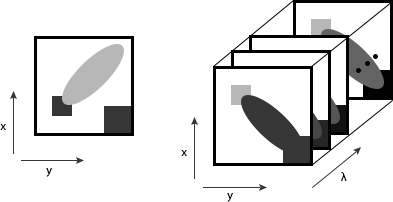
\includegraphics[scale=0.25]{spectral_image}
            \caption{Examples of a monochrome image (left) and a spectral image (right).}
        \end{figure}

        An ``RGB'' image can be considered spectral, where we have $f=3$, with a 
        spectral bin for the red, green and blue regions of the visible spectrum.

        Finally some literature refer to \textit{multispectral} and \textit{hyperspectral} images (which may be 
        referenced such as in \cite{Luthman:2015:hyperspectralImager} and \cite{Bioucas-Dias:2012:unmixingOverview}), 
        which are simply special cases of a spectral image. A multispectral image refers to a small number of spectral 
        bands (such as 5) and a hyperspectral image refers to a large number of spectral bands (such as 50). Intuitively, 
        we can think of the difference between multispectral and hyperspectral in terms of their spectra: a 
        multispectral image should be thought of as having quantised spectra (histograms), whereas a hyperspectral 
        image can be thought of as attempting to approximate the continuous spectra.


    \section{Aims of the project} \label{sec:what_are_we_trying_to_do}
        Nowadays computer vision techniques are used in abundance to aid medical diagnosis, and they are used by doctors 
        to help provide more accurate and earlier diagnoses. This is clearly an area of interest, as such tools 
        may help improve, or even save lives where we wouldn't have been able to do so in the past. 

        In this project we consider using spectral images (recall that this includes RGB images) for medical purposes 
        and we wish to segment the image to indicate different regions of interest, typically which would indicate some form of 
        disease or abnormality. The problem can easily be described mathematically: given an arbitrary spectral image 
        $I : \bb{N}_w \times \bb{N}_h \times \bb{N}_f \rightarrow \bb{N}$ and a set of possible classes 
        $\cl{C}$, we want to output a \textit{pixel labelling} $\cl{P} : \bb{N}_w \times \bb{N}_h 
        \rightarrow \cl{C}$ that correctly identifies regions of the image according to $\cl{C}$. Succinctly 
        put, we want to perform \textit{image segmentation}, on (noisy) medical (spectral) images.

        The motivation for this project comes from use of a the hyperspectral imager for use with contrast agents 
        \cite{Luthman:2015:hyperspectralImager}. The aim is that the imager can be used to identify the presence of 
        fluorescent contrast agents, some of which have a negative binding response to cancerous cells in the oesophagus, 
        thus allowing cancerous tissues to be identified. The Biological and Soft Systems group from the physics department 
        at Cambridge have kindly given me some images taken with the imager used by Luthman et al \cite{Luthman:2015:hyperspectralImager},
        which we will refer to as ``\siris dataset''.

        To summarise, we wish to produce a system capable of producing a pixel labelling from a spectral image. The 
        pixel labelling will depend highly on the data and so we would likely wish to learn from some examples.

    \section{Possible solutions}
        As we will be looking to segment images, we will need to identify regions of the image based on the data 
        available. One approach that we might take is to try and identify some properties manually, For example one 
        possible solution in \siris dataset is to explicitly find the spectra of \textit{endmembers} (the 
        fluorescents) in the images, then use a \textit{spectral unmixing} algorithm \cite{keshava2003survey} such as 
        constrained least squares. The output of a spectral unmixing algorithm will identify the proportions of endmembers 
        present at each given point \cite{Luthman:2015:hyperspectralImager}.

        An alternative would be to utilising machine learning methods, where one might hope to learn 
        relationships within the data through supervised learning. Such a system may be more versatile, be able to 
        solve many similar problems and may not be constrained to a specific problem. For example, the spectral unmixing 
        solution above requires the endmembers to be measurable, requiring significant work prior to putting the data 
        through the algorithm. We would hope by using machine learning that we can avoid such additional work, and even 
        solve problems where the `endmembers' are not separable with explicitly measurable spectra.

    \section{Related work}
        Medical imaging is an active research area and will likely be for a long time. Medical imaging is ubiquitous in 
        hospitals and an essential tool to aid doctors in diagnosing a patient. Along with medical imaging comes 
        medical image analysis, where image processing methods are used to give more information to doctors which they 
        may not be able to see with the naked eye. The task of image segmentation is important in medicine: illnesses and 
        viruses are commonly localised, only affecting parts of tissues and identification of which parts of tissues 
        are healthy or not is important to successful treatment.

        Plenty of work and research that has gone into image segmentation, and it is a common technique used in 
        medical imaging. It can be implemented using a variety of methods such as classifiers, thresholding and region growing
        \cite{pham2000current}. However traditional (non machine learning) methods seem to be loosing traction, with  
        few papers written in this decade readily available, paling in comparison to the vast number of machine learning 
        based literature. 

        Recently neural networks have seen a major dominance with regards to machine learning; within medical 
        imaging other areas of machine learning are still finding success, with whole books still dedicated to the 
        topic \cite{criminisi2013decision}. True to the current trend, there is plenty of current work utilising 
        neural networks in medical imaging. For example they have been successfully applied to segment different 
        regions of the brain, such as `white matter', `gray matter', and `cerebrospinal fluid' \cite{zhao2016segmenting},
        and similarly for segmentation of brain tumours \cite{zhao2016multiscale}.

        However, other machine learning methods are still of interest and random forests are still an active area of 
        research within medical imaging and computer vision \cite{conjeti2016supervised}, especially because of their 
        simplicity and lack of complexity, which can potentially make them very efficient \cite{criminisi2012decision}.

        SegNet \cite{badrinarayanan2015segnet2} is a deep convolutional neural network architecture built on top of Caffe 
        \cite{jia2014caffe} for pixel wise labelling, and provides some inspiration for the project. SegNet uses 
        supervised learning to train the neural network using known labelled images. In normal operation it takes some 
        image as input and outputs a pixel labelling. Bayesian SegNet which is an extension 
        to SegNet, includes an additional output image, which is a mapping of uncertainty in each pixel labelling, 
        something that is desirable in our own system. The Caffe implementation includes support for OpenCL 
        (an open source GPU programming language), allowing for an efficient implementation. This is realised by 
        applying it to run on a real-time video stream, with 360 by 480 resolution. Whilst this implementation isn't 
        necessarily geared towards medical purposes, it could certainly be utilised for a medical application, and 
        is a good example of a system solving the more general problem of image segmentation/pixel labelling.











%%%%%%%%%%%%%%%%%%%%%%%%%%%%%%%%%%%%%%%%%%%%%%%%%%%%%%%%%%%%%%%%%%%%%%%%%%%%%%%%%%%%%%%%%%%%%%%%%%%%%%%%%%%%%%%%%%%%%%%%
% the preparation

\cleardoublepage
\chapter{Preparation}
    In this section we will introduce the area of image segmentation and how we may perform segmentation. Then we 
    introduce decision trees and explain the supervised learning methods of random forests and neural networks. In the 
    second half of the chapter 
    we outline the design with a requirements analysis, pipeline overview, what tools we will use and a backup strategy 
    to avoid loosing any work.

    From a list of machine learning algorithms: State Vector Machine \cite{klein2004lagrange}, \cite{law2006simple}, 
    Hidden Markov Models \cite{seymore1999learning}, k Nearest Neighbour \cite{cunningham2007k}, Random Forests 
    \cite{criminisi2013decision}, and Neural Networks \cite{heaton2008introduction}, we decided on two algorithms that 
    would be useful in our case, Random Forests and Neural Networks. So a Random Forests library will be implemented and 
    the Encog library will be employed for Neural Networks in Java \cite{JMLR:v16:heaton15a}.



    \section{An introduction to image segmentation}
        Image segmentation concerns splitting an image into connected subsets, in some meaningful way. Despite being an 
        ill-posed problem with no `best' segmentation, we often have some desired segmentation that we would 
        like our system to perform. The term `ground truth' is used to refer to a hand labelled image, in which an 
        accuracy of 100\% is assumed. When training a supervised learning system we will provide some number of ground 
        truth images. 

        More formally if we let $\Omega$ be the set of pixels in some image, a valid image segmentation is $(S_1, ..., 
        S_n)$ for some $n \in \bb{N}$ which satisfy the following:

        \begin{align}
            \Omega = \bigcup\limits_{i=1}^n S_i \\
            S_i \cap S_j = \emptyset && \forall i,j \in \{1,\ldots,n\}. i \neq j 
        \end{align}

        where each $S_i$ is connected, which means that there is a path between any two pixels of $S_i$. 
        A path may take steps of one pixel up, left, down or right \cite{PAL19931277}. 

        There are a number of ways that we may try to perform an image segmentation. One such method consists of 
        finding the edges present in an image, by using the zero crossings of a gradient operator, 
        such as the Laplacian. Furthermore, we may want to look at edges at different scales, which suggests blurring 
        the image before taking the gradient operator, leading to the Laplacian of Gaussian operator, as discussed by 
        Pal et al \cite{PAL19931277}. An even simpler method would be to use grey level threshold, where we segment 
        images depending on whether they fall above or below some threshold, also discussed by Pal et al \cite{PAL19931277}.

        Finally, the method that we will use is to generate some pixel labelling $\cl{P}:\Omega \rightarrow \cl{C}$ as 
        described in section \ref{sec:what_are_we_trying_to_do}. This implicitly defines a segmentation of an image 
        via regions of similarly classed pixels.




    \section{Supervised learning for classification} \label{sec:supervised_learning}
        Before discussing any machine learning methods we first need to define some terminology that we will be using. 
        In classification we are given a \textit{feature vector} (or \textit{instance}) $\vc{x} = (x_1, x_2, ..., x_d) 
        \in \bb{R}^d$ and a set of classes $\cl{C} = \{C_1, C_2, ..., C_n\}$. We want to \textit{learn} some 
        hypothesis $h:\bb{R}^d \rightarrow \cl{C}$ which maps instances to their classification. To learn 
        what hypotheses are appropriate we rely on a \textit{training sequence} $\vc{s} = ((\vc{x}_1, c_1), 
        (\vc{x}_2, c_2), ..., (\vc{x}_m, c_m))$, which makes the method \textit{supervised}. We usually assume that 
        the training sequence is noisy, which can be sufficiently represented by noise solely attributed to the classes of $\vc{s}$ 
        (that is $c_1, ..., c_m$). So we can consider each of the $c_i$ to be a random variable, and hence consider 
        $\vc{s}$ to be a random variable. Two sensible approaches that we might take to choosing some hypothesis $h$ 
        either picking

        \begin{align}
            h_{\ML} = \argmax_{h\in\cl{H}} \Pr(h | \vc{s})
            \label{eq:max_likelihood}
        \end{align}

        or picking

        \begin{align}
            h_{\MAP} = \argmax_{h\in\cl{H}} \Pr(\vc{s} | h) \Pr(h)
            \label{eq:max_a_posteriori}
        \end{align} 

        where $\ML$ stands for \textit{maximum likelihood} and $\MAP$ stands for \textit{maximum a-posteriori}. The $\MAP$ 
        hypothesis allows the prior $\Pr(h)$ to be used (indicating some prior knowledge about the hypothesis), however 
        if $\Pr(h)$ is uniform, then the $\ML$ and $\MAP$ hypothesis are easily shown to be equivalent using Bayes' theorem. 
        These two methods of picking a hypothesis are referred to as Bayesian learning methods; as we look to maximise 
        likelihoods. We will see that this is not the only way of picking a suitable hypothesis. \cite{russell1995modern}

        We often also see that some hypothesis will take the form of $h':\bb{R}^d \rightarrow (\cl{C} \rightarrow [0,1])$, 
        that is it gives a probability distribution over classes. We can then simply set 
        
        \begin{align}
            h(\vc{x}) = \argmax_{c\in\cl{C}} h'(\vc{x})(c)
            \label{eq:weird_hyp}
        \end{align}

        which is `the most likely class'.

        



    \section{Decision trees and random forests} \label{sec:rand_forest}
        This section defines what a decision tree is, how it can be used in supervised learning and then extend it to 
        the concept of random forests. As mentioned in section \ref{sec:supervised_learning} we opt for a hypothesis 
        which outputs a probability distribution over classes as opposed to a single class, which 
        can be used to give a single class.

        \subsection{Introduction to decision trees} \label{sec:intro_decision_trees}
            Decision trees consist of a simple binary tree structure. Intuitively, we think about asking a question at each 
            node, making a decision on which child node to traverse to and eventually reach some conclusion at a leaf node, such 
            as in figure \ref{fig:intuitive_tree}. We can use this model for the situation described in section 
            \ref{sec:supervised_learning}, where we are allowed to `ask a question' about the feature vector at each 
            decision node and leaf nodes consider

            \begin{figure}
                \centering

                \tikzset{QuestionNode/.style = { rectangle, rounded corners, shade, 
                              top color = white, bottom color = blue!50!black!20, 
                              draw = blue!40!black!60, very thick, text ragged },
                          EdgeNodeStyle/.style = {draw = none}, above,
                          EmptyNode/.style = {draw = none}}
                \begin{tikzpicture}
                    [
                        sibling distance = 3cm,
                        level distance = 4cm,
                        edge from parent/.style = {draw, arrows = ->},
                        level 1/.style = {sibling distance = 3cm, level distance = 3cm},
                        level 2/.style = {sibling distance = 1.5cm, level distance = 3cm},
                    ]
                    \node [QuestionNode] {Blond hair?}
                        child {
                            node [QuestionNode] {Brown hair?}
                            child {
                                node [EmptyNode] {$\vdots$}
                                edge from parent
                                  node [EdgeNodeStyle, left] {no}
                            }
                            child {
                                node [EmptyNode] {$\vdots$}
                                edge from parent
                                  node [EdgeNodeStyle, right] {yes}
                            }
                            edge from parent node [EdgeNodeStyle, left] {no}
                        }   
                        child {
                            node [QuestionNode] {Blue eyes?}
                            child {
                                node [EmptyNode] {$\vdots$}
                                edge from parent
                                  node [EdgeNodeStyle, left] {no}
                            }
                            child {
                                node [EmptyNode] {$\vdots$}
                                edge from parent
                                  node [EdgeNodeStyle, right] {yes}
                            }
                            edge from parent node [EdgeNodeStyle, right] {yes}
                        };
                    \end{tikzpicture}

                \caption{Example of (part of) a tree used to classify humans.}
                \label{fig:intuitive_tree}
            \end{figure}

            More formally we can define a decision tree $T$ for classification, which has a set of states $Q \subseteq 
            \bb{N}$, such that if $i \in Q$ is a decision node, then it has children $2i, 2i+1 \in Q$. 

            \begin{figure}
                \centering
                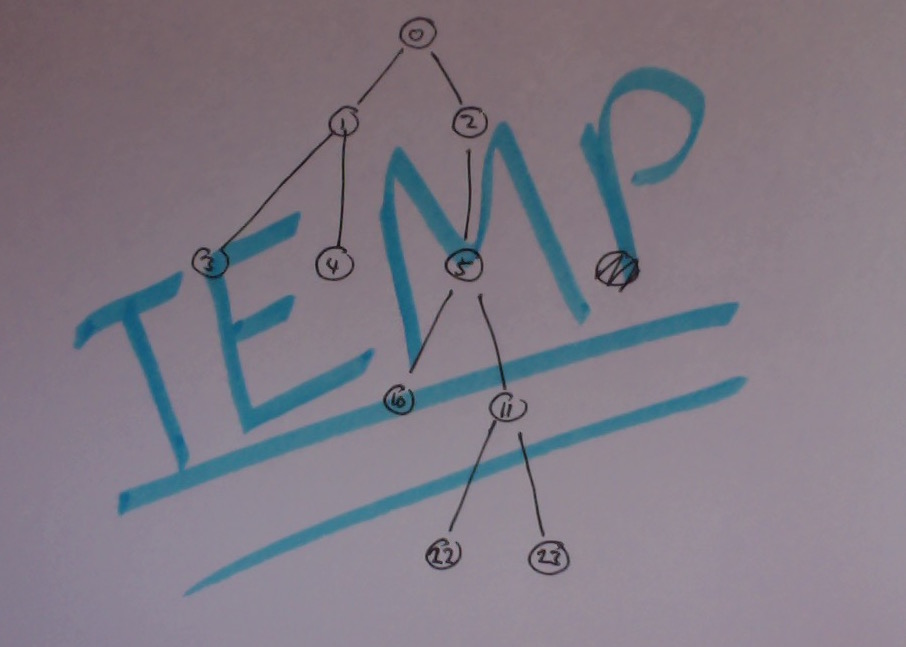
\includegraphics[scale=0.8]{tree_node_labels}
                \caption[Example of node numberings in a decision tree.]{Example of node numberings in a decision tree. Reproduced from Criminisini et al \cite{criminisi2012decision}.}
            \end{figure}

            For our model we specify some function $f:\bb{R}^d \times \cl{T} \rightarrow \bb{B}$, where $\cl{T}$ is some 
            parameter space and is used to specify a function from $\bb{R}^d$ to $\bb{B}$ at each decision node.  
            $f$ is called a \textit{weak learner} or a \textit{split function}. In a decision tree for each state $i \in Q$ we have 
            some associated $\vc{\theta}_i \in \cl{T}$ called a \textit{split parameter}, used to specify 
            $f_i(\vc{x}) = f(\vc{x}; \vc{\theta}_i)$. The function $f_i : \bb{R}^d \rightarrow \bb{B}$ is then used to 
            make a decision to traverse to either state $2i$ or $2i+1$ next. Finally when we hit a leaf node $j \in Q$ we need 
            to specify some probability distribution $p_j:\cl{C} \rightarrow [0,1]$ where:

            \begin{align}
                p_j(c) = \Pr(\vc{x} \in c | \vc{x} \text{ traversed to } j \text{ in } T).
            \end{align}

            As it can be seen in Figure \ref{fig:decision_tree_classify} in order to classify some instance $\vc{x}$ using a 
            decision tree $T$ we simply traverse $T$ using $f_i$ at each node $i \in Q$ to make a decision whether 
            to traverse to $2i$ or $2i+1$ next. We usually use the following rule: if $f_i(\vc{x}) = 0$ then traverse to 
            $2i$, otherwise if $f_i(\vc{x}) = 1$ then traverse to $2i+1$. \cite{criminisi2013decision}

            \begin{figure}
                \centering
                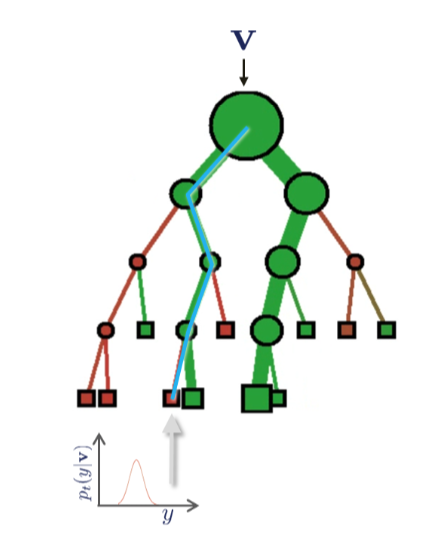
\includegraphics[scale=0.5]{tree_example_classification}
                \caption[Example of how some instance $\vc{v}$ would be classified using a decision tree.]{Example of how some instance $\vc{v}$ would be classified using a decision tree. Partially reproduced from Criminisini et al \cite{criminisi2012decision}.}
                \label{fig:decision_tree_classify}
            \end{figure}

        \subsection{Training a decision tree}
            When training a decision tree we use a greedy approach, to train at each node optimally. A 
            greedy approach is necessary because optimising over all possible trees is a computationally infeasible task (it is an 
            NP-complete problem to decide if a tree is optimal). So consider having a set of states $Q$ and for each state
            $i \in Q$ we want to learn the split parameter $\vc{\theta}_i \in \cl{T}$. Let $\vc{s}_i$ be the training 
            sequence that $i$ is trained on. It is sensible to set $\vc{s_0}=\vc{s}$. 

            We first define the \textit{entropy} of a training sequence:

            \begin{align}
                H(s) = - \sum_{c\in\cl{C}} p(c) \log_2 (p(c)).
                \label{eq:training_seq_entropy}
            \end{align}

            We assume feature vectors in $s$ to be unique for ease of notation and let:

            \begin{align}
                p(c) = \frac{\left| \{\vc{v}\ |\ c' = c \land (\vc{v},c') \in S \} \right|}{\left| S \right|},
                \label{eq:empirical_distribution}
            \end{align}
            
            which is the empirical probability of a training sample vector in $s$ being classified as $c$. Now we define 
            a left and right split of $\vc{s}$, using some split parameter $\vc{\theta} \in \cl{T}$ according to our weak 
            learner $f$ as follows:

            \begin{align}
                L(\vc{s},\vc{\theta}) & = \{ (\vc{x}, c) \in s | f(\vc{x}, \vc{\theta}) = 0 \}  \label{eq:left_split}\\
                R(\vc{s},\vc{\theta}) & = \{ (\vc{x}, c) \in s | f(\vc{x}, \vc{\theta}) = 1 \}. \label{eq:right_split}
            \end{align}

            Consider the \textit{information gain} $I$ for performing a split according to $\vc{\theta}$ of 

            \begin{align}
                I(\vc{s}, \vc{\theta}) = H(\vc{s}) - \frac{1}{|\vc{s}|} \left( |L(\vc{s}, \vc{\theta})| H(L(\vc{s}, \vc{\theta})) 
                                                                          + |R(\vc{s}, \vc{\theta})| H(R(\vc{s}, \vc{\theta})) \right).
                \label{eq:information_gain}
            \end{align} 

            We now have a way of picking $\vc{\theta}_i$ at each node

            \begin{align} 
                \vc{\theta}_i = \argmax_{\theta\in\cl{T}} I(\vc{s}_i, \vc{\theta}).
            \end{align} 

            Once we have found a $\vc{\theta}_i$ we then set $s_{2i} = L(\vc{s}_i, \vc{\theta}_i)$ and 
            $s_{2i+1} = R(\vc{s}_i, \vc{\theta}_i)$, which allows us to begin training at node $0$ with $\vc{s}_0 = \vc{s}$ 
            and then recursively train down the tree. \cite{criminisi2013decision}


        \subsection{Moving swiftly on to random forests} \label{sec:moving_swiftly_onto_forests}
            Decision trees have a couple major disadvantages, which are solved by extending the concept to random 
            forests. The first problem is that we learn $\vc{\theta}_i$ using

            \begin{align} 
                \vc{\theta}_i = \argmax_{\theta\in\cl{T}} I(\vc{s}_i, \vc{\theta}),
            \end{align}

            which is a problematic because $|\cl{T}|$ may be infinite. We resolve this by randomly sampling $\cl{T}$ with 
            $\rho$ values, so let $\cl{T}_\rho = \{ \vc{\theta}_i^{(1)}, ..., \vc{\theta}_i^{(\rho)} \} \subseteq \cl{T}$.
            So we instead set 

            \begin{align} 
                \vc{\theta}_i = \argmax_{\theta\in\cl{T}_\rho} I(\vc{s}_i, \vc{\theta}),
            \end{align}            

            when training at node $i$, where $\rho$ \textit{fresh} samples are taken from $\cl{T}$ per node. This 
            optimisation is called the \textit{random node optimisation}. The second problem with decision trees is that 
            we can easily over fit and also we cannot solve some XOR/parity problems \cite{criminisi2013decision}. We 
            can address this by using a \textit{forest} of decision trees. A forest $F$ is a set of trees, 
            that is $F = \{ T_1, T_2, ..., T_k \}$, where each $T_\ell$ is trained separately with training sequence 
            $\vc{s}$. As we randomly train each tree on the same data, it is reasonable to say that the probability of 
            any given tree in $F$ to be `correct' tree is equally likely. Hence we set $\Pr(T_\ell) = 1/k$ for each 
            $\ell$. Finally, when we wish to classify some instance $\vc{x}$ using a random forest we output 

            \begin{align}
                p(c) & = \Pr(\vc{x} \in c) \\
                    & = \sum_{\ell=1}^k \Pr(\vc{x} \in c, T_\ell) \\
                    & = \sum_{\ell=1}^k \Pr(\vc{x} \in c | T_\ell) \Pr(T_\ell) \\
                    & = \frac{1}{k} \sum_{\ell=1}^k \Pr(\vc{x} \in c | T_\ell)
            \end{align}

            where each $\Pr(\vc{x} \in c | T_\ell)$ is the probability obtained by traversing each tree. \cite{criminisi2013decision}

            Therefore, to classify using a forest, we just take an average of the outputs from the trees. 





    \section{Neural networks} \label{sec:neuralnetworkdef}
        We now move on to describe a second method of supervised learning, neural networks. We begin 
        by defining a single neuron and how it operates, then develop the idea into a neural network. Then the 
        general idea of how to train a neural network is explained.

            \subsection{Neural network definitions}

                A neuron has a number of inputs, say $\{a_i\}$, for each $a_i$ there is a weight $w_i$ and each neuron also has 
                some \textit{bias} value $b$, as can be seen in Figure \ref{fig:neuron}. Each node has some 
                \textit{activation function} $\sigma$, to which the weighted sum of inputs $z = \sum_{i} a_iw_i + b$ is input. 
                The value of the neurons output $a'$ called the \textit{activation} is:
                
                \begin{align}
                    a' = \sigma(z) = \sigma\left(\sum_i a_iw_i + b \right).
                \end{align}

                \begin{figure}
                    \centering
                    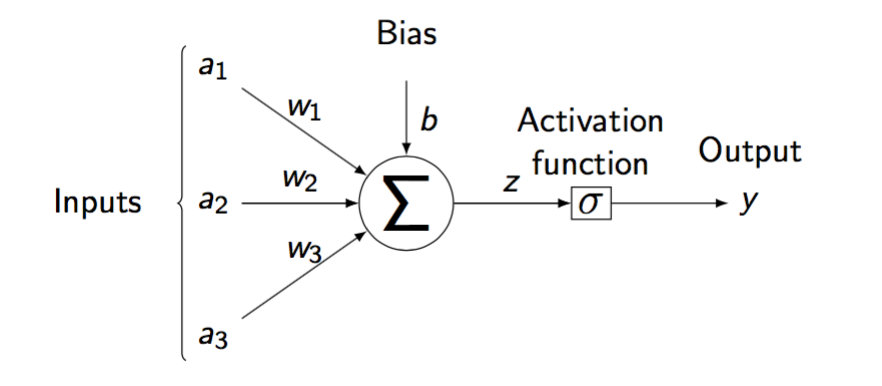
\includegraphics[scale=0.5]{neuron}
                    \caption{Example of an (artificial) neuron, with 3 inputs.}
                    \label{fig:neuron}
                \end{figure}

                A commonly used activation function is the \textit{sigmoid} function:

                \begin{align}
                    \sigma(z) = \frac{1}{1+e^{-z}}.
                \end{align}

                A single neuron is pretty basic by itself and cannot solve parity problems, however they can be organised into 
                networks to compute more complex functions, where the output of one neuron is the input of another. A typical 
                arrangement is a \textit{feedforward} network (one without any loops), with the neurons arranged into layers. 

                \begin{figure}
                    \centering
                    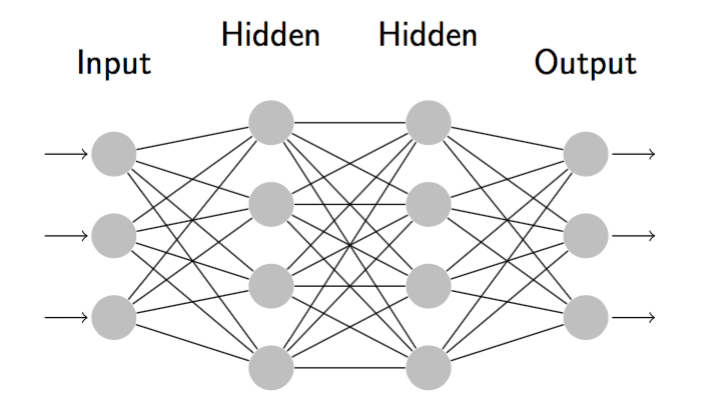
\includegraphics[scale=0.5]{neuralnetwork}
                    \caption{Example of a feed forward neural network.}
                    \label{fig:neuron}
                \end{figure}

                The input to each neuron in layer $L+1$ is the activation (output) of neurons in layer $L$.
                Let $a_j^L$ be the activation of the $j$th neuron in layer $L$, with bias $b_j^L$. The weights from layer $L$ to 
                layer $L+1$, from the $j$th node of layer $L$ to the $i$th node of layer $L+1$ are denoted $w_{ji}^{L+1}$. The 
                situation can be visualised in Figure \ref{fig:feedforwardNetwork}.

                \begin{figure}
                    \centering
                    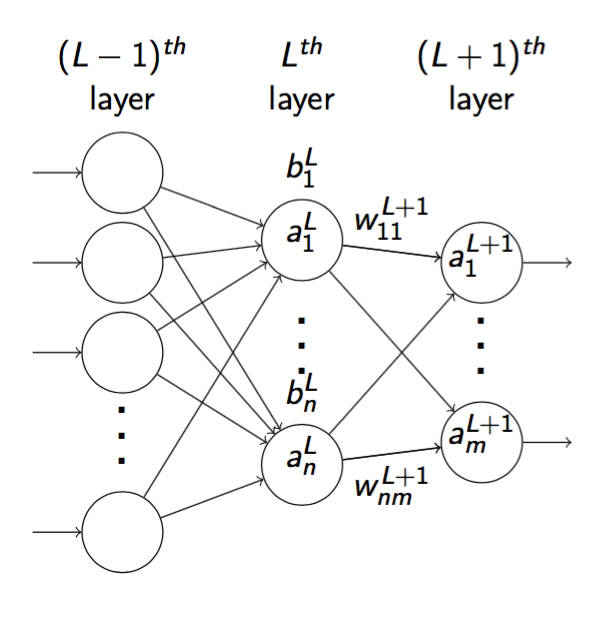
\includegraphics[scale=0.5]{neuralnetwork_with_vals}
                    \caption[A neural network showing internal values.]{A neural network showing internal values. Computation of values in the network is known as \textit{forward propagation}.}
                    \label{fig:feedforwardNetwork}
                \end{figure}


            \subsection{Training a neural network}

                A feed forward neural network can be thought of as a function $f:\bb{R}^n \times \bb{R}^m \rightarrow \bb{R}^k$, 
                if there $n$ inputs to the network, $k$ outputs and $m$ weights. Suppose we have a training sequence $\vc{s} = 
                ((\vc{x}_1, \vc{y}_1), ..., (\vc{x}_\ell, \vc{y}_\ell)$ where for each $1\leq i \leq \ell$ we have $\vc{x}_i 
                \in \bb{R}^n$ and $\vc{y}_j \in \bb{R}^k$. 

                It is possible to find a suitable hypothesis $h:\bb{R}^n \rightarrow \bb{R}^k$ 
                where $h(\cdot) = f(\cdot;\vc{w})$ for a suitable $\vc{w}$. Suitable values of $\vc{w}$ can be found by 
                solving an optimisation problem such as:
                
                \begin{align}
                    \vc{w} = \argmin_{\vc{w}'} \sum\limits_{i=1}^\ell E(\vc{w'})
                    \label{eq:optimisation}
                \end{align}

                where the function $E$ depends on what assumptions are made about the properties of noise in the training sequence and the prior 
                distribution of weights $\Pr(\vc{w})$. One common function is 

                \begin{align}
                    E(\vc{w}) =  \frac{1}{2} \sum\limits_{i=1}^\ell || \vc{y}_i - f(\vc{x}_i;\vc{w}) || ^2
                \end{align}

                where we assume a Gaussian noise on each $\vc{y}_i$. Optimising over this can be shown to give the maximum
                likelihood hypothesis from equation \ref{eq:maximum_likelihood}\cite{russell1995modern}.
                Another common choice for $E$ is:

                \begin{align}
                    E(\vc{w}) = \frac{\alpha}{2} ||\vc{w}||^2 + \frac{\beta}{2} \sum\limits_{i=1}^\ell \frac{1}{2} || \vc{y}_i - f(\vc{x}_i;\vc{w}) || ^2
                 \end{align}

                 which can be shown to yeild the maximum a-posteriori hypothesis from equation \ref{eq:max_a_posteriori},
                 under the assumption of a Gaussian distribution on the prior $\Pr(\vc{w})$.
                 This method is known as the \textit{weight decay} method, and will keep the weights in $\vc{w}$ small, 
                 so that the neural network doesn't over fit itself to a single input. The parameters $\alpha$ and $\beta$ can be 
                 found \cite{eq:max_likelihood}, but is beyond the scope of this dissertation. \cite{russell1995modern}

                 The optimisation problem of finding a solution to \ref{eq:optimisation} can be found using an algorithm 
                 such as the method of conjugate gradients \cite{shewchuk1994introduction}, or gradient descent. 
                 The value of $\partial E/\partial \vc{w}$ is often needed in such algorithms, and can be computed using 
                 an algorithm such as backpropagaton. \cite{russell1995modern}


        








    \section{Requirements analysis}
        Now that the relevance in context has been discussed, we move onto the design of the system. Firstly we carefully consider 
        the requirements of the system. This is important to begin identifying the work that needs to be undertaken 
        and where potential risks lie. 

        \begin{table}[H]
            \begin{minipage}{\textwidth}
                \begin{tabular}{lccc}
                    \hline 
                        \textbf{Goal Requirement} & \textbf{Priority} & \textbf{Risk} & \textbf{Difficulty} \\
                    \hline 
                        Build a random forests machine learning library       & High      & Low         & Medium    \\
                        Incorporate a neural network library (Encog)          & High      & Medium      & Medium    \\
                        Image segmentation via pixel labelling                & High      & Low         & Low       \\
                        Suitably model and account for image noise            & Medium    & High        & High      \\ 
                        Train the pixel labelling system on real data         & High      & High        & Low       \\
                        Build an aid to help create training sets             & Medium    & Low         & Low       \\
                        Model uncertainty and output in a certainty map       & Medium    & Medium      & Medium    \\
%                        Optimise algorithms and implementations for GPU       & Low       & High        & High      \\
                    \hline  
                \end{tabular}
            \end{minipage}
            \caption{High level goals and desired outcomes for the project.}
        \end{table}


    \section{System Design}
        This section outlines the overview of the whole system, where we begin with a work flow diagram comprising of 
        files and system components. The system is then divided into its separate components and used to define an 
        interface, along with a brief description of each module in addition to defining inputs and outputs. The formats of the files 
        that the user should input can be found in appendix \ref{app:file_formats}.


        \subsection{Pipeline/Overview}
            An overview of what we want the system to do (the pipeline of the system) is illustrated in terms of the 
            files input and output by different modules of the system. In the system overview in Figure \ref{fig:system_overview}, 
            blue boxes are code modules and red boxes represent files.

            \begin{figure}[H]
                \centering
                    \scalebox{0.55}{ 
                        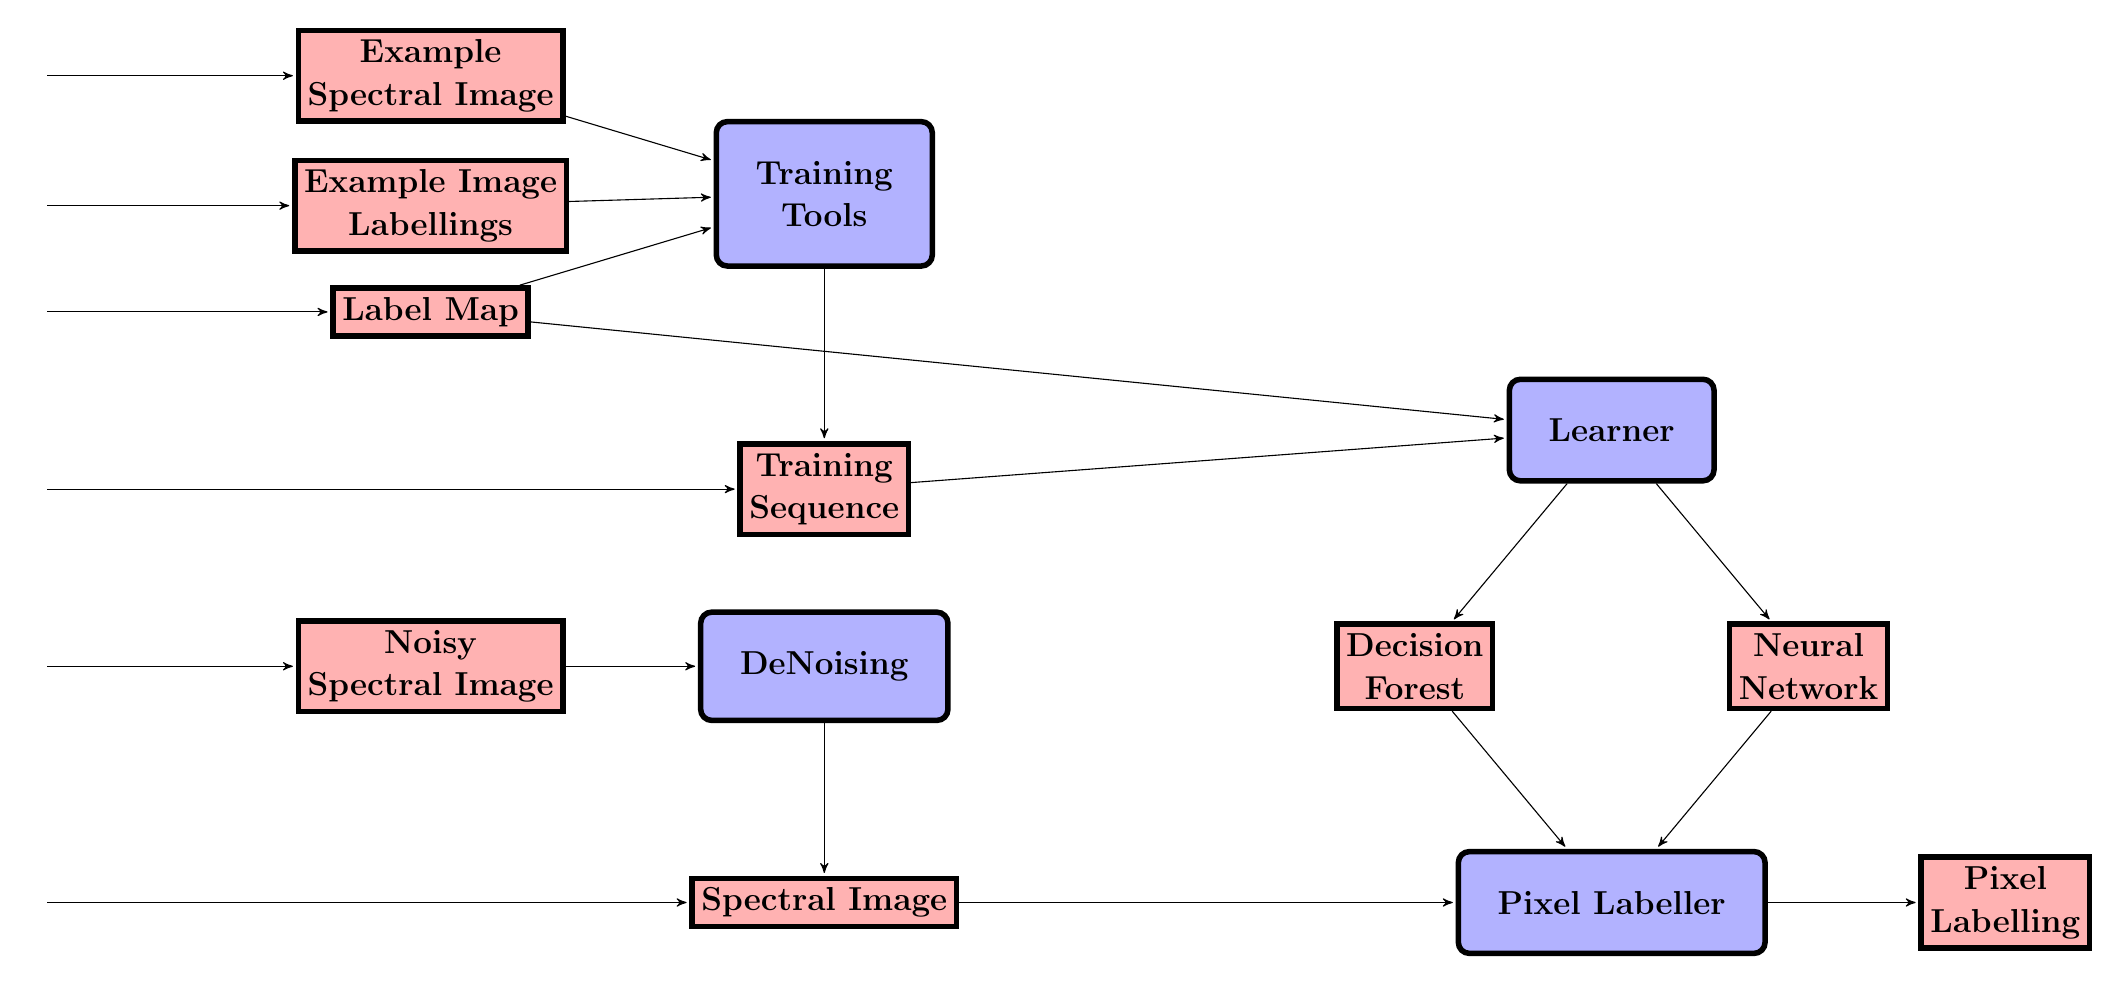
\begin{tikzpicture}[node distance=2cm,>=stealth',bend angle=45,auto]

                            \tikzstyle{commonNode}=[thick, font=\ttfamily\large\bf, align=center, line width=2pt, draw=black]
                            \tikzstyle{module}=[commonNode, rectangle, rounded corners, fill=blue!30, inner sep=5mm]
                            \tikzstyle{file}=[commonNode, fill=red!30]
                            \tikzstyle{unusedModule}=[module, fill=blue!10, line width=0pt]
                            \tikzstyle{unusedFile}=[file, fill=red!10, line width=0pt]
                            \tikzstyle{intermediateFile}=[file, dash pattern=on 3pt off 3pt, line width=1pt]

                            \begin{scope}
                                % Spacing the nodes out
                                \def \hspacing {5}
                                \def \vspacing {3}
                                \def \indent {0.25}

                                % Background
                                %\fill[black!20, rounded corners=10] (-0.75*\hspacing, 0.5*\vspacing) rectangle (4.5*\hspacing, 5.5*\vspacing);

                                % Title
                                %\node at (-0.75*\hspacing+\indent, 5.5*\vspacing-\indent) [anchor=north west] {\textbf{System Overview}};

                                % Inputs
                                \node at (-1*\hspacing, 4.5*\vspacing) (EHIin) {};
                                \node at (-1*\hspacing, 3.95*\vspacing) (EILin) {};
                                \node at (-1*\hspacing, 3.5*\vspacing) (LMin) {};
                                \node at (-1*\hspacing, 2.75*\vspacing) (TSin) {};
                                \node at (-1*\hspacing, 2*\vspacing) (NHIin) {};
                                \node at (-1*\hspacing, 1*\vspacing) (HIin) {};

                                % Files and modules
                                \node at (0*\hspacing, 4.5*\vspacing) [file]    (EHI)     {Example \\ Spectral Image}
                                    edge  [pre]   (EHIin);
                                \node at (0*\hspacing, 3.95*\vspacing)   [file]    (EIL)     {Example Image \\ Labellings}
                                    edge  [pre]   (EILin);
                                \node at (0*\hspacing, 3.5*\vspacing) [file]    (LM)      {Label Map}
                                    edge  [pre]   (LMin);
                                \node at (1*\hspacing, 4*\vspacing)   [module]  (TT)      {Training \\ Tools}
                                    edge  [pre]   (EHI)
                                    edge  [pre]   (EIL)
                                    edge  [pre]   (LM);
                                \node at (1*\hspacing, 2.75*\vspacing)   [file]    (TS)      {Training \\ Sequence}
                                    edge  [pre]   (TSin)
                                    edge  [pre]   (TT);
                                \node at (3*\hspacing, 3*\vspacing)   [module]  (L)       {Learner}
                                    edge  [pre]   (LM)
                                    edge  [pre]   (TS);
                                \node at (2.5*\hspacing, 2*\vspacing) [file]    (F)       {Decision \\ Forest}
                                    edge  [pre]   (L);
                                \node at (3.5*\hspacing, 2*\vspacing) [file]    (NN)      {Neural \\ Network}
                                    edge  [pre]   (L);
                                \node at (0*\hspacing, 2*\vspacing)   [file]    (NHI)     {Noisy \\ Spectral Image}
                                    edge  [pre]   (NHIin);
                                \node at (1*\hspacing, 2*\vspacing)   [module]  (DB)      {DeNoising}
                                    edge  [pre]   (NHI);
                                \node at (1*\hspacing, 1*\vspacing)   [file]    (HI)      {Spectral Image}
                                    edge  [pre]   (HIin)
                                    edge  [pre]   (DB);
                                \node at (3*\hspacing, 1*\vspacing)   [module]  (C)       {Pixel Labeller}
                                    edge  [pre]   (F)
                                    edge  [pre]   (NN)
                                    edge  [pre]   (HI);
                                \node at (4*\hspacing, 1*\vspacing)   [file]    (PL)      {Pixel \\ Labelling}
                                    edge  [pre]   (C);
                            \end{scope}

                            % \begin{pgfonlayer}{background}
                                
                            % \end{pgfonlayer}
                        \end{tikzpicture}
                    }

                \caption{Overview of the system and its intended use.}
                \label{fig:system_overview}
            \end{figure}   



        \subsection{Interface/Usage}
            We will not only allow usage for each module separately, but also for combined steps that will 
            avoid unnecessary intermediate files to be produced. For our interface the diagrams that consisted 
            of red boxes for files and blue boxes for code modules are extended to denote files/modules unused in a given function 
            by a faded/duller colour. An intermediate file that isn't saved during some function is marked by a 
            regularly bright, but dashed border. It should be assumed that an intermediate file need not be provided 
            by the user.




            \subsubsection{Training Tools}
                The training tools' function is to take an example class map, pixel labelling and spectral image (see 
                appendix \ref{app:file_formats} for how their formats). From this `ground truth' we will output a 
                training sequence as specified in appendix \ref{app:file_formats}. The use of this function is to 
                generate vast quantities of training data with minimal effort.

                \begin{figure}[H]
                    \centering
                        \scalebox{0.55}{ 
                            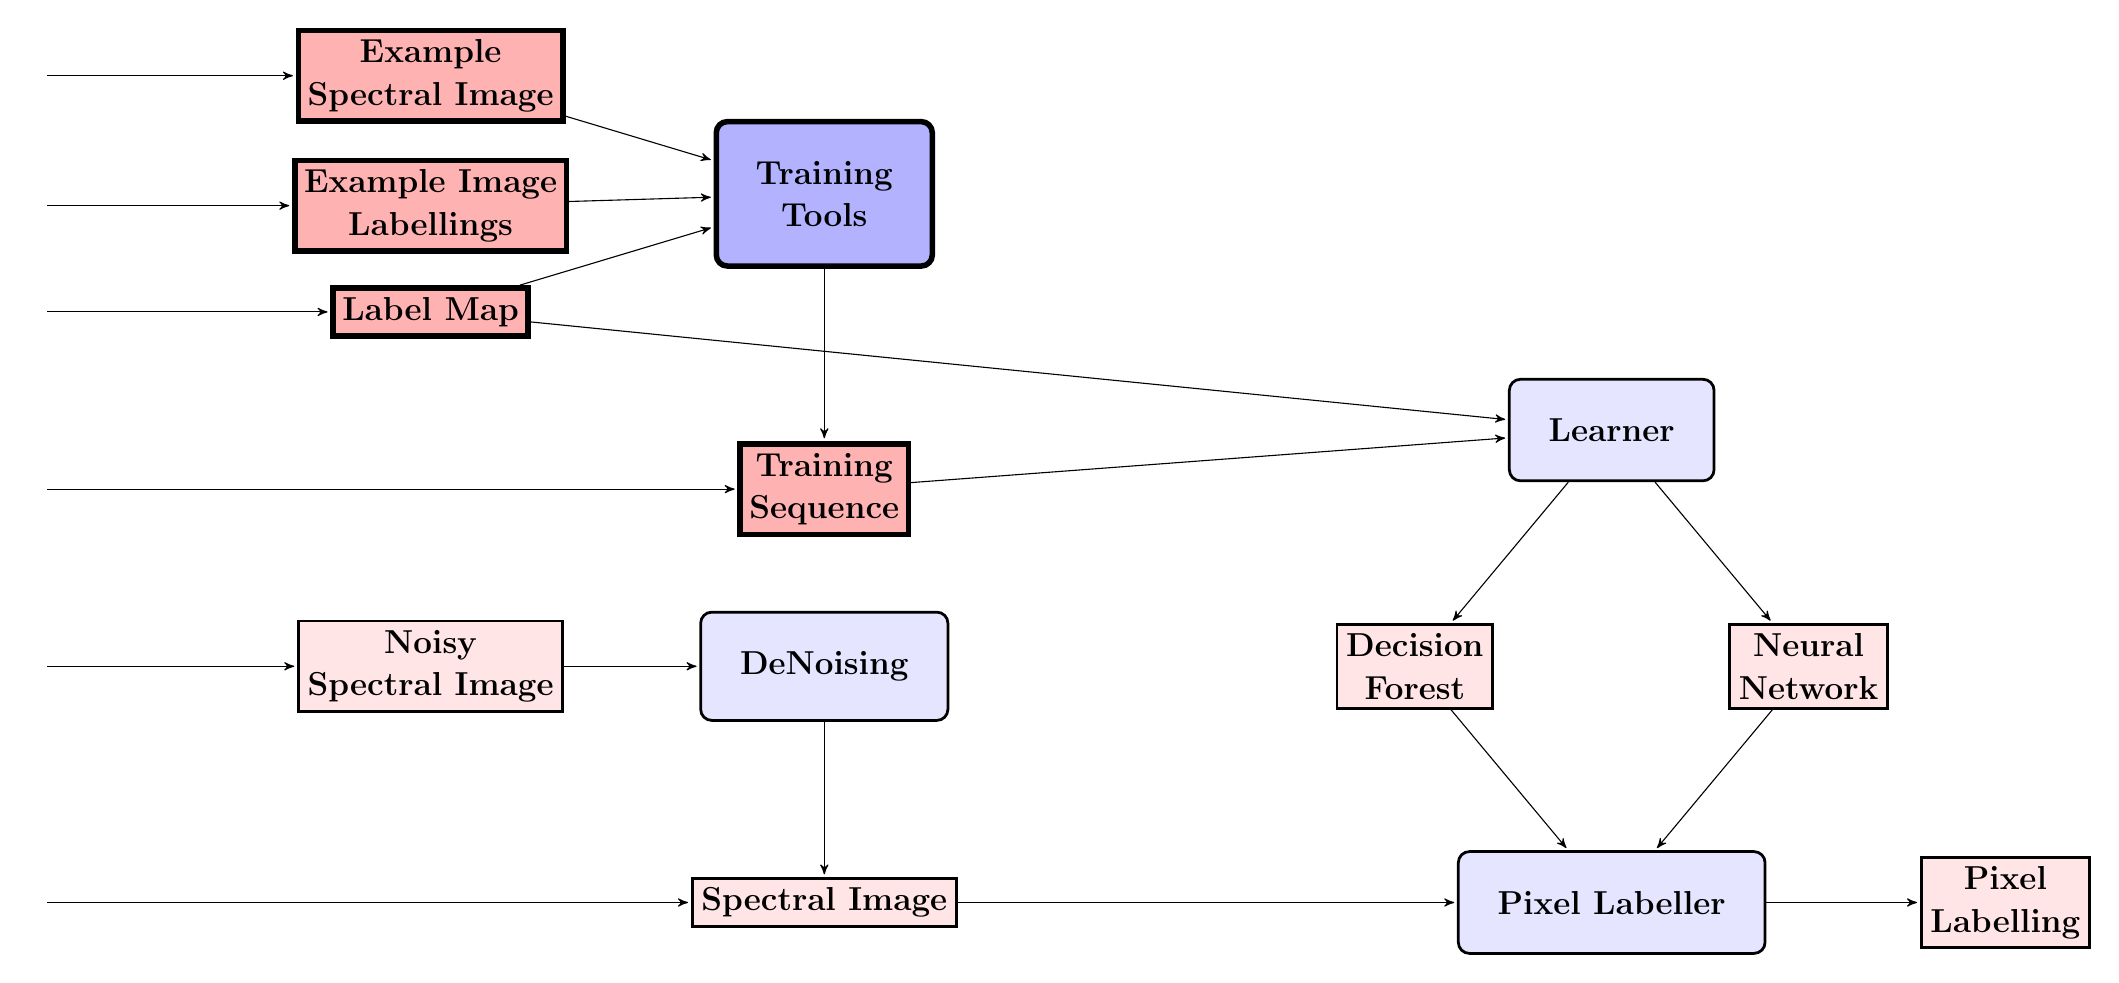
\begin{tikzpicture}[node distance=2cm,>=stealth',bend angle=45,auto]

                                \tikzstyle{commonNode}=[thick, font=\ttfamily\large\bf, align=center, line width=2pt, draw=black]
                                \tikzstyle{module}=[commonNode, rectangle, rounded corners, fill=blue!30, inner sep=5mm]
                                \tikzstyle{file}=[commonNode, fill=red!30]
                                \tikzstyle{unusedModule}=[module, fill=blue!10, line width=1pt]
                                \tikzstyle{unusedFile}=[file, fill=red!10, line width=1pt]
                                \tikzstyle{intermediateFile}=[file, dash pattern=on 3pt off 3pt, line width=1pt]

                                \begin{scope}
                                    % Spacing the nodes out
                                    \def \hspacing {5}
                                    \def \vspacing {3}
                                    \def \indent {0.25}

                                    % Background
                                    %\fill[black!20, rounded corners=10] (-0.75*\hspacing, 0.5*\vspacing) rectangle (4.5*\hspacing, 5.5*\vspacing);

                                    % Title
                                    %\node at (-0.75*\hspacing+\indent, 5.5*\vspacing-\indent) [anchor=north west] {\textbf{System Overview}};

                                    % Inputs
                                    \node at (-1*\hspacing, 4.5*\vspacing) (EHIin) {};
                                    \node at (-1*\hspacing, 3.95*\vspacing) (EILin) {};
                                    \node at (-1*\hspacing, 3.5*\vspacing) (LMin) {};
                                    \node at (-1*\hspacing, 2.75*\vspacing) (TSin) {};
                                    \node at (-1*\hspacing, 2*\vspacing) (NHIin) {};
                                    \node at (-1*\hspacing, 1*\vspacing) (HIin) {};

                                    % Files and modules
                                    \node at (0*\hspacing, 4.5*\vspacing) [file]    (EHI)     {Example \\ Spectral Image}
                                        edge  [pre]   (EHIin);
                                    \node at (0*\hspacing, 3.95*\vspacing)   [file]    (EIL)     {Example Image \\ Labellings}
                                        edge  [pre]   (EILin);
                                    \node at (0*\hspacing, 3.5*\vspacing) [file]    (LM)      {Label Map}
                                        edge  [pre]   (LMin);
                                    \node at (1*\hspacing, 4*\vspacing)   [module]  (TT)      {Training \\ Tools}
                                        edge  [pre]   (EHI)
                                        edge  [pre]   (EIL)
                                        edge  [pre]   (LM);
                                    \node at (1*\hspacing, 2.75*\vspacing)   [file]    (TS)      {Training \\ Sequence}
                                        edge  [pre]   (TSin)
                                        edge  [pre]   (TT);
                                    \node at (3*\hspacing, 3*\vspacing)   [unusedModule]  (L)       {Learner}
                                        edge  [pre]   (LM)
                                        edge  [pre]   (TS);
                                    \node at (2.5*\hspacing, 2*\vspacing) [unusedFile]    (F)       {Decision \\ Forest}
                                        edge  [pre]   (L);
                                    \node at (3.5*\hspacing, 2*\vspacing) [unusedFile]    (NN)      {Neural \\ Network}
                                        edge  [pre]   (L);
                                    \node at (0*\hspacing, 2*\vspacing)   [unusedFile]    (NHI)     {Noisy \\ Spectral Image}
                                        edge  [pre]   (NHIin);
                                    \node at (1*\hspacing, 2*\vspacing)   [unusedModule]  (DB)      {DeNoising}
                                        edge  [pre]   (NHI);
                                    \node at (1*\hspacing, 1*\vspacing)   [unusedFile]    (HI)      {Spectral Image}
                                        edge  [pre]   (HIin)
                                        edge  [pre]   (DB);
                                    \node at (3*\hspacing, 1*\vspacing)   [unusedModule]  (C)       {Pixel Labeller}
                                        edge  [pre]   (F)
                                        edge  [pre]   (NN)
                                        edge  [pre]   (HI);
                                    \node at (4*\hspacing, 1*\vspacing)   [unusedFile]    (PL)      {Pixel \\ Labelling}
                                        edge  [pre]   (C);
                                \end{scope}

                                % \begin{pgfonlayer}{background}
                                    
                                % \end{pgfonlayer}
                            \end{tikzpicture}
                        }

                    \caption{Overview of the training tools function.}
                \end{figure} 



            \subsubsection{Train}
                The train function will take a training sequence and then produce either a forest file or a neural 
                network file. These files will be output to be used later by the pixel labeller.

                \begin{figure}[H]
                    \centering
                        \scalebox{0.55}{ 
                            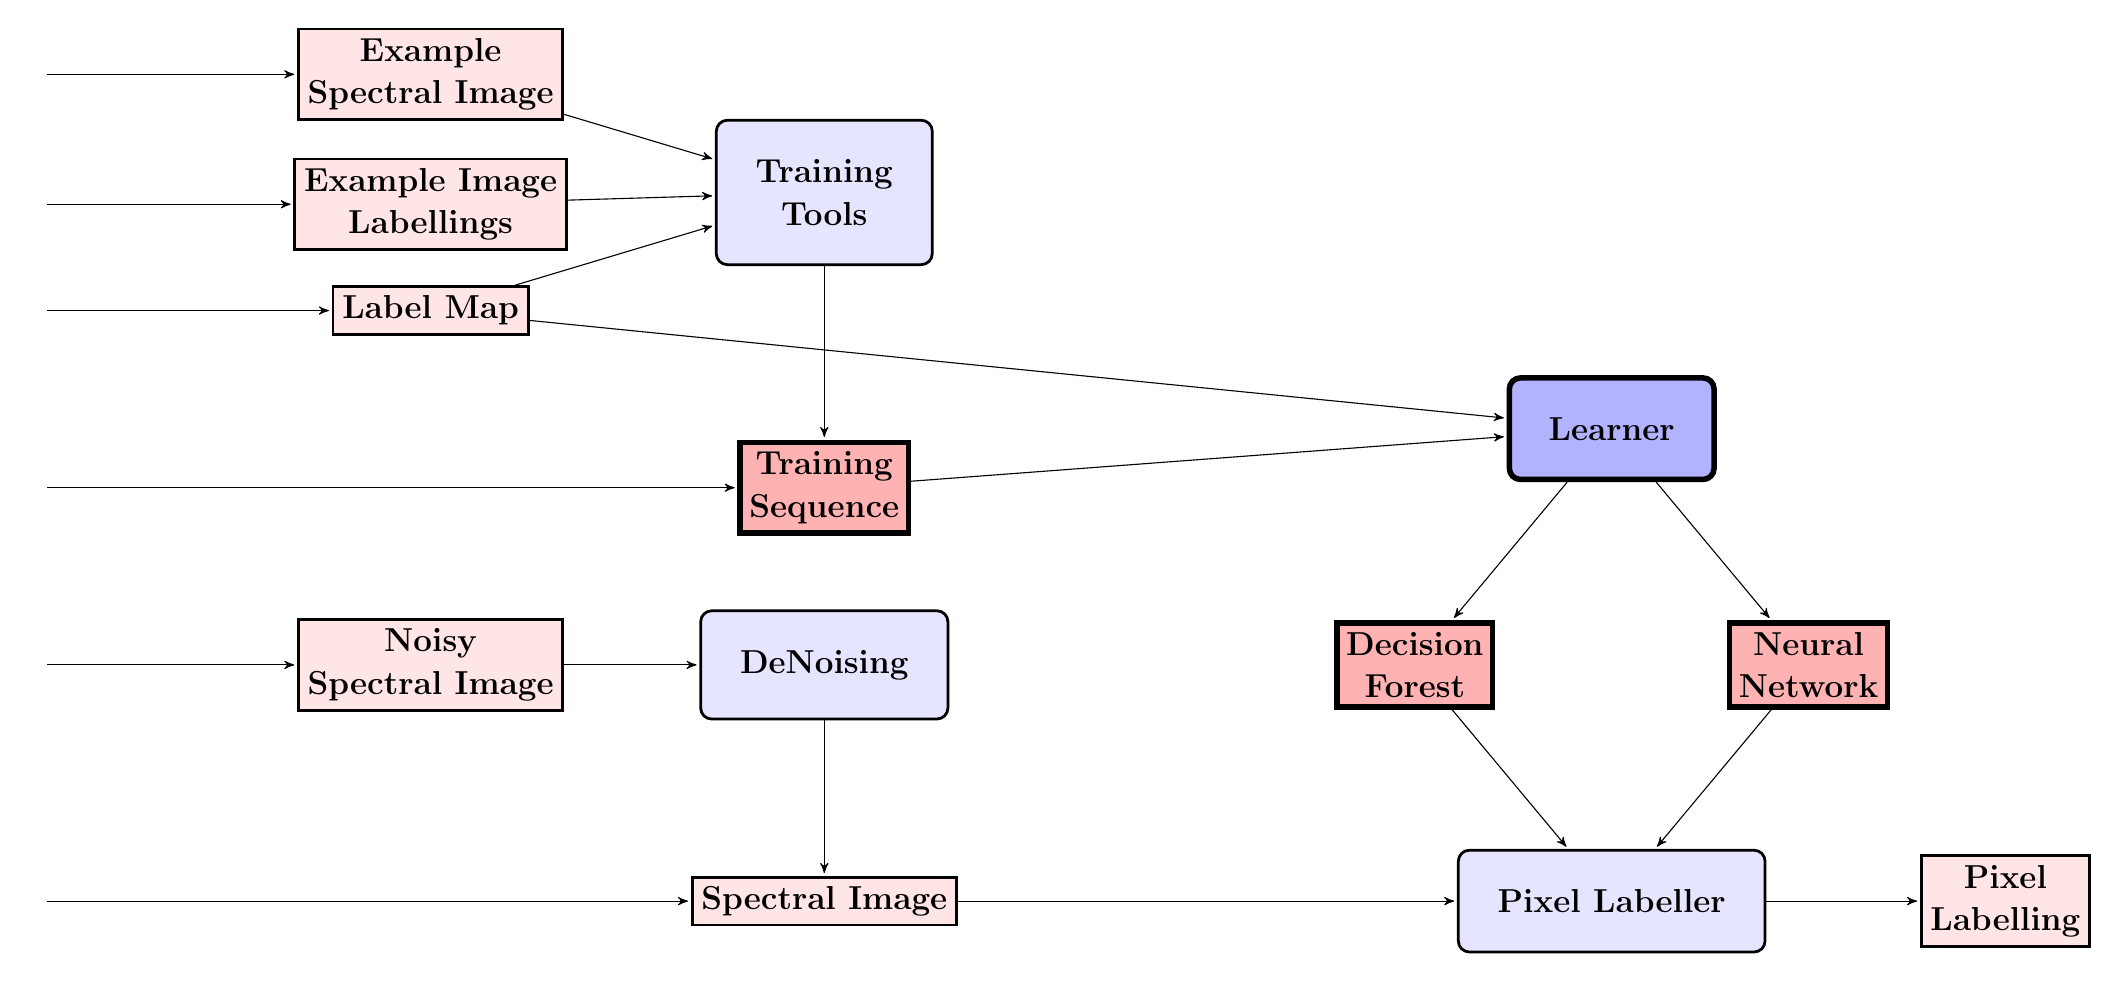
\begin{tikzpicture}[node distance=2cm,>=stealth',bend angle=45,auto]

                                \tikzstyle{commonNode}=[thick, font=\ttfamily\large\bf, align=center, line width=2pt, draw=black]
                                \tikzstyle{module}=[commonNode, rectangle, rounded corners, fill=blue!30, inner sep=5mm]
                                \tikzstyle{file}=[commonNode, fill=red!30]
                                \tikzstyle{unusedModule}=[module, fill=blue!10, line width=1pt]
                                \tikzstyle{unusedFile}=[file, fill=red!10, line width=1pt]
                                \tikzstyle{intermediateFile}=[file, dash pattern=on 3pt off 3pt, line width=1pt]

                                \begin{scope}
                                    % Spacing the nodes out
                                    \def \hspacing {5}
                                    \def \vspacing {3}
                                    \def \indent {0.25}

                                    % Background
                                    %\fill[black!20, rounded corners=10] (-0.75*\hspacing, 0.5*\vspacing) rectangle (4.5*\hspacing, 5.5*\vspacing);

                                    % Title
                                    %\node at (-0.75*\hspacing+\indent, 5.5*\vspacing-\indent) [anchor=north west] {\textbf{System Overview}};

                                    % Inputs
                                    \node at (-1*\hspacing, 4.5*\vspacing) (EHIin) {};
                                    \node at (-1*\hspacing, 3.95*\vspacing) (EILin) {};
                                    \node at (-1*\hspacing, 3.5*\vspacing) (LMin) {};
                                    \node at (-1*\hspacing, 2.75*\vspacing) (TSin) {};
                                    \node at (-1*\hspacing, 2*\vspacing) (NHIin) {};
                                    \node at (-1*\hspacing, 1*\vspacing) (HIin) {};

                                    % Files and modules
                                    \node at (0*\hspacing, 4.5*\vspacing) [unusedFile]    (EHI)     {Example \\ Spectral Image}
                                        edge  [pre]   (EHIin);
                                    \node at (0*\hspacing, 3.95*\vspacing)   [unusedFile]    (EIL)     {Example Image \\ Labellings}
                                        edge  [pre]   (EILin);
                                    \node at (0*\hspacing, 3.5*\vspacing) [unusedFile]    (LM)      {Label Map}
                                        edge  [pre]   (LMin);
                                    \node at (1*\hspacing, 4*\vspacing)   [unusedModule]  (TT)      {Training \\ Tools}
                                        edge  [pre]   (EHI)
                                        edge  [pre]   (EIL)
                                        edge  [pre]   (LM);
                                    \node at (1*\hspacing, 2.75*\vspacing)   [file]    (TS)      {Training \\ Sequence}
                                        edge  [pre]   (TSin)
                                        edge  [pre]   (TT);
                                    \node at (3*\hspacing, 3*\vspacing)   [module]  (L)       {Learner}
                                        edge  [pre]   (LM)
                                        edge  [pre]   (TS);
                                    \node at (2.5*\hspacing, 2*\vspacing) [file]    (F)       {Decision \\ Forest}
                                        edge  [pre]   (L);
                                    \node at (3.5*\hspacing, 2*\vspacing) [file]    (NN)      {Neural \\ Network}
                                        edge  [pre]   (L);
                                    \node at (0*\hspacing, 2*\vspacing)   [unusedFile]    (NHI)     {Noisy \\ Spectral Image}
                                        edge  [pre]   (NHIin);
                                    \node at (1*\hspacing, 2*\vspacing)   [unusedModule]  (DB)      {DeNoising}
                                        edge  [pre]   (NHI);
                                    \node at (1*\hspacing, 1*\vspacing)   [unusedFile]    (HI)      {Spectral Image}
                                        edge  [pre]   (HIin)
                                        edge  [pre]   (DB);
                                    \node at (3*\hspacing, 1*\vspacing)   [unusedModule]  (C)       {Pixel Labeller}
                                        edge  [pre]   (F)
                                        edge  [pre]   (NN)
                                        edge  [pre]   (HI);
                                    \node at (4*\hspacing, 1*\vspacing)   [unusedFile]    (PL)      {Pixel \\ Labelling}
                                        edge  [pre]   (C);
                                \end{scope}

                                % \begin{pgfonlayer}{background}
                                    
                                % \end{pgfonlayer}
                            \end{tikzpicture}
                        }

                    \caption{Overview of the train function.}
                \end{figure} 



            \subsubsection{Learn From Example}
                The \textit{learn from example} function is a composite of the training tools and train functions. This will 
                take the same inputs as the training tools function, but instead will immediately use the training 
                sequence produced to train a random forest or neural network. The training sequence is not saves in the 
                process. 

                \begin{figure}[H]
                    \centering
                        \scalebox{0.55}{ 
                            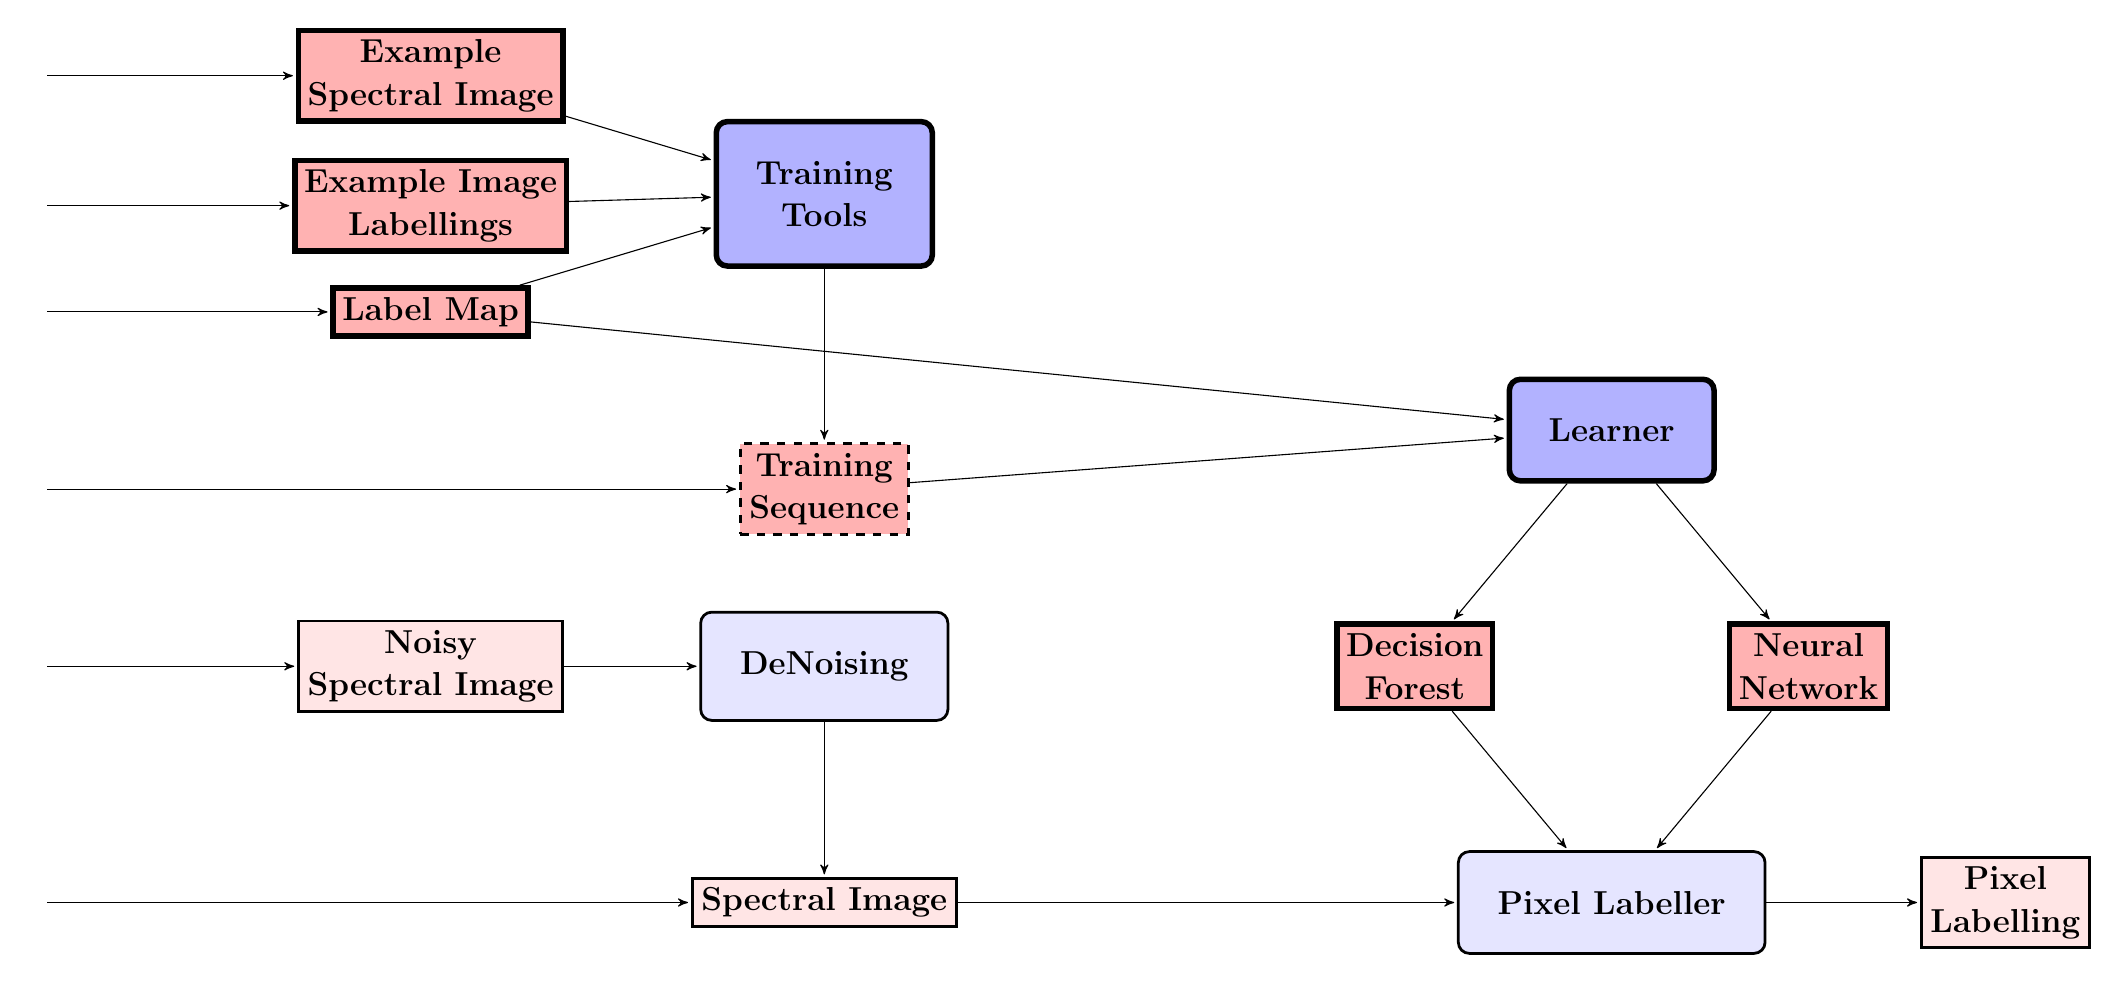
\begin{tikzpicture}[node distance=2cm,>=stealth',bend angle=45,auto]

                                \tikzstyle{commonNode}=[thick, font=\ttfamily\large\bf, align=center, line width=2pt, draw=black]
                                \tikzstyle{module}=[commonNode, rectangle, rounded corners, fill=blue!30, inner sep=5mm]
                                \tikzstyle{file}=[commonNode, fill=red!30]
                                \tikzstyle{unusedModule}=[module, fill=blue!10, line width=1pt]
                                \tikzstyle{unusedFile}=[file, fill=red!10, line width=1pt]
                                \tikzstyle{intermediateFile}=[file, dash pattern=on 3pt off 3pt, line width=1pt]

                                \begin{scope}
                                    % Spacing the nodes out
                                    \def \hspacing {5}
                                    \def \vspacing {3}
                                    \def \indent {0.25}

                                    % Background
                                    %\fill[black!20, rounded corners=10] (-0.75*\hspacing, 0.5*\vspacing) rectangle (4.5*\hspacing, 5.5*\vspacing);

                                    % Title
                                    %\node at (-0.75*\hspacing+\indent, 5.5*\vspacing-\indent) [anchor=north west] {\textbf{System Overview}};

                                    % Inputs
                                    \node at (-1*\hspacing, 4.5*\vspacing) (EHIin) {};
                                    \node at (-1*\hspacing, 3.95*\vspacing) (EILin) {};
                                    \node at (-1*\hspacing, 3.5*\vspacing) (LMin) {};
                                    \node at (-1*\hspacing, 2.75*\vspacing) (TSin) {};
                                    \node at (-1*\hspacing, 2*\vspacing) (NHIin) {};
                                    \node at (-1*\hspacing, 1*\vspacing) (HIin) {};

                                    % Files and modules
                                    \node at (0*\hspacing, 4.5*\vspacing) [file]    (EHI)     {Example \\ Spectral Image}
                                        edge  [pre]   (EHIin);
                                    \node at (0*\hspacing, 3.95*\vspacing)   [file]    (EIL)     {Example Image \\ Labellings}
                                        edge  [pre]   (EILin);
                                    \node at (0*\hspacing, 3.5*\vspacing) [file]    (LM)      {Label Map}
                                        edge  [pre]   (LMin);
                                    \node at (1*\hspacing, 4*\vspacing)   [module]  (TT)      {Training \\ Tools}
                                        edge  [pre]   (EHI)
                                        edge  [pre]   (EIL)
                                        edge  [pre]   (LM);
                                    \node at (1*\hspacing, 2.75*\vspacing)   [intermediateFile]    (TS)      {Training \\ Sequence}
                                        edge  [pre]   (TSin)
                                        edge  [pre]   (TT);
                                    \node at (3*\hspacing, 3*\vspacing)   [module]  (L)       {Learner}
                                        edge  [pre]   (LM)
                                        edge  [pre]   (TS);
                                    \node at (2.5*\hspacing, 2*\vspacing) [file]    (F)       {Decision \\ Forest}
                                        edge  [pre]   (L);
                                    \node at (3.5*\hspacing, 2*\vspacing) [file]    (NN)      {Neural \\ Network}
                                        edge  [pre]   (L);
                                    \node at (0*\hspacing, 2*\vspacing)   [unusedFile]    (NHI)     {Noisy \\ Spectral Image}
                                        edge  [pre]   (NHIin);
                                    \node at (1*\hspacing, 2*\vspacing)   [unusedModule]  (DB)      {DeNoising}
                                        edge  [pre]   (NHI);
                                    \node at (1*\hspacing, 1*\vspacing)   [unusedFile]    (HI)      {Spectral Image}
                                        edge  [pre]   (HIin)
                                        edge  [pre]   (DB);
                                    \node at (3*\hspacing, 1*\vspacing)   [unusedModule]  (C)       {Pixel Labeller}
                                        edge  [pre]   (F)
                                        edge  [pre]   (NN)
                                        edge  [pre]   (HI);
                                    \node at (4*\hspacing, 1*\vspacing)   [unusedFile]    (PL)      {Pixel \\ Labelling}
                                        edge  [pre]   (C);
                                \end{scope}

                                % \begin{pgfonlayer}{background}
                                    
                                % \end{pgfonlayer}
                            \end{tikzpicture}
                        }

                    \caption{Overview of the \textit{learn from example} function.}
                \end{figure} 




            \subsubsection{Pixel Labeller}
                The pixel labeller could be considered the primary part of the system. It uses the pixel labeller 
                module to label a spectral image using a trained forest/neural network.

                \begin{figure}[H]
                    \centering
                        \scalebox{0.55}{ 
                            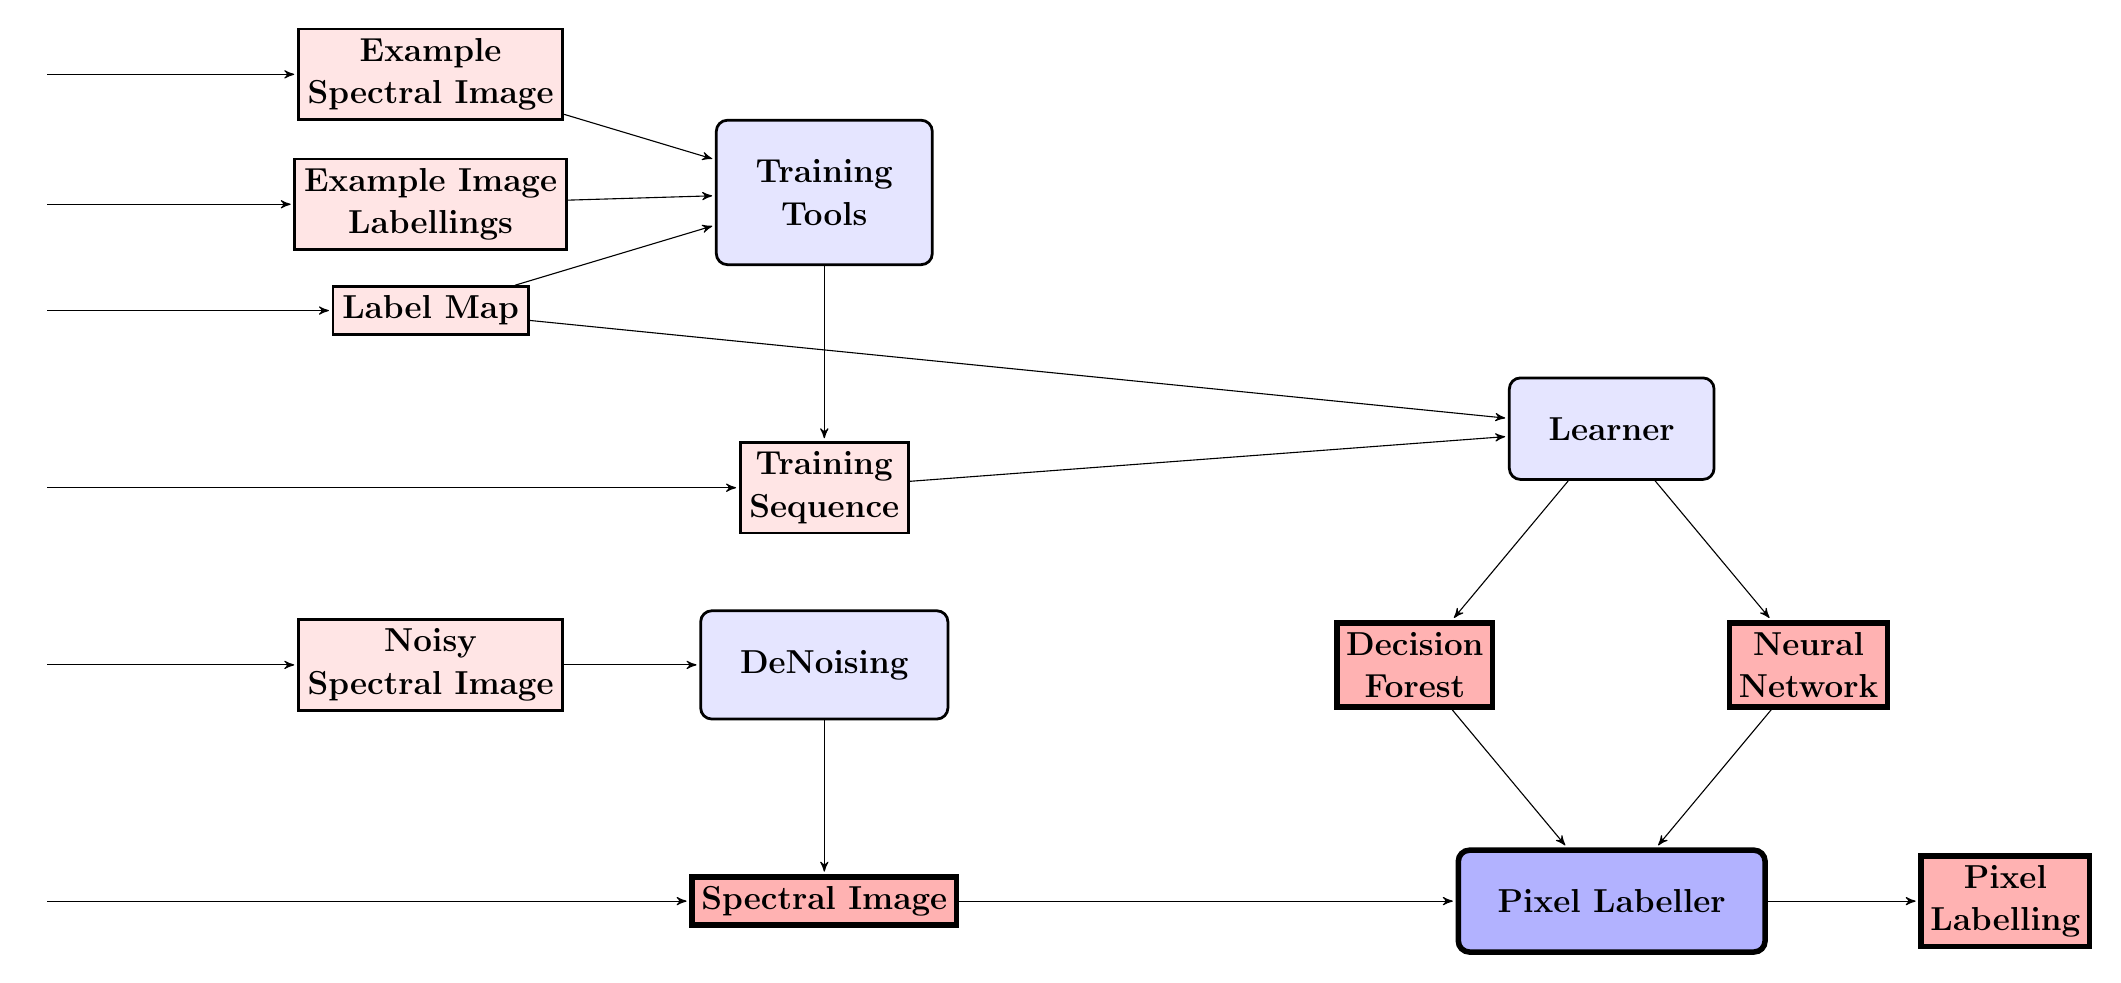
\begin{tikzpicture}[node distance=2cm,>=stealth',bend angle=45,auto]

                                \tikzstyle{commonNode}=[thick, font=\ttfamily\large\bf, align=center, line width=2pt, draw=black]
                                \tikzstyle{module}=[commonNode, rectangle, rounded corners, fill=blue!30, inner sep=5mm]
                                \tikzstyle{file}=[commonNode, fill=red!30]
                                \tikzstyle{unusedModule}=[module, fill=blue!10, line width=1pt]
                                \tikzstyle{unusedFile}=[file, fill=red!10, line width=1pt]
                                \tikzstyle{intermediateFile}=[file, dash pattern=on 3pt off 3pt, line width=1pt]

                                \begin{scope}
                                    % Spacing the nodes out
                                    \def \hspacing {5}
                                    \def \vspacing {3}
                                    \def \indent {0.25}

                                    % Background
                                    %\fill[black!20, rounded corners=10] (-0.75*\hspacing, 0.5*\vspacing) rectangle (4.5*\hspacing, 5.5*\vspacing);

                                    % Title
                                    %\node at (-0.75*\hspacing+\indent, 5.5*\vspacing-\indent) [anchor=north west] {\textbf{System Overview}};

                                    % Inputs
                                    \node at (-1*\hspacing, 4.5*\vspacing) (EHIin) {};
                                    \node at (-1*\hspacing, 3.95*\vspacing) (EILin) {};
                                    \node at (-1*\hspacing, 3.5*\vspacing) (LMin) {};
                                    \node at (-1*\hspacing, 2.75*\vspacing) (TSin) {};
                                    \node at (-1*\hspacing, 2*\vspacing) (NHIin) {};
                                    \node at (-1*\hspacing, 1*\vspacing) (HIin) {};

                                    % Files and modules
                                    \node at (0*\hspacing, 4.5*\vspacing) [unusedFile]    (EHI)     {Example \\ Spectral Image}
                                        edge  [pre]   (EHIin);
                                    \node at (0*\hspacing, 3.95*\vspacing)   [unusedFile]    (EIL)     {Example Image \\ Labellings}
                                        edge  [pre]   (EILin);
                                    \node at (0*\hspacing, 3.5*\vspacing) [unusedFile]    (LM)      {Label Map}
                                        edge  [pre]   (LMin);
                                    \node at (1*\hspacing, 4*\vspacing)   [unusedModule]  (TT)      {Training \\ Tools}
                                        edge  [pre]   (EHI)
                                        edge  [pre]   (EIL)
                                        edge  [pre]   (LM);
                                    \node at (1*\hspacing, 2.75*\vspacing)   [unusedFile]    (TS)      {Training \\ Sequence}
                                        edge  [pre]   (TSin)
                                        edge  [pre]   (TT);
                                    \node at (3*\hspacing, 3*\vspacing)   [unusedModule]  (L)       {Learner}
                                        edge  [pre]   (LM)
                                        edge  [pre]   (TS);
                                    \node at (2.5*\hspacing, 2*\vspacing) [file]    (F)       {Decision \\ Forest}
                                        edge  [pre]   (L);
                                    \node at (3.5*\hspacing, 2*\vspacing) [file]    (NN)      {Neural \\ Network}
                                        edge  [pre]   (L);
                                    \node at (0*\hspacing, 2*\vspacing)   [unusedFile]    (NHI)     {Noisy \\ Spectral Image}
                                        edge  [pre]   (NHIin);
                                    \node at (1*\hspacing, 2*\vspacing)   [unusedModule]  (DB)      {DeNoising}
                                        edge  [pre]   (NHI);
                                    \node at (1*\hspacing, 1*\vspacing)   [file]    (HI)      {Spectral Image}
                                        edge  [pre]   (HIin)
                                        edge  [pre]   (DB);
                                    \node at (3*\hspacing, 1*\vspacing)   [module]  (C)       {Pixel Labeller}
                                        edge  [pre]   (F)
                                        edge  [pre]   (NN)
                                        edge  [pre]   (HI);
                                    \node at (4*\hspacing, 1*\vspacing)   [file]    (PL)      {Pixel \\ Labelling}
                                        edge  [pre]   (C);
                                \end{scope}

                                % \begin{pgfonlayer}{background}
                                    
                                % \end{pgfonlayer}
                            \end{tikzpicture}
                        }

                    \caption{Overview of the pixel labeller function.}
                \end{figure} 




            \subsubsection{De-Noiser}
                The de-noiser function attempts to reduce the effect of noise on the image. It takes a spectral 
                image as input and outputs the de-noised spectral image.

                \begin{figure}[H]
                    \centering
                        \scalebox{0.55}{ 
                            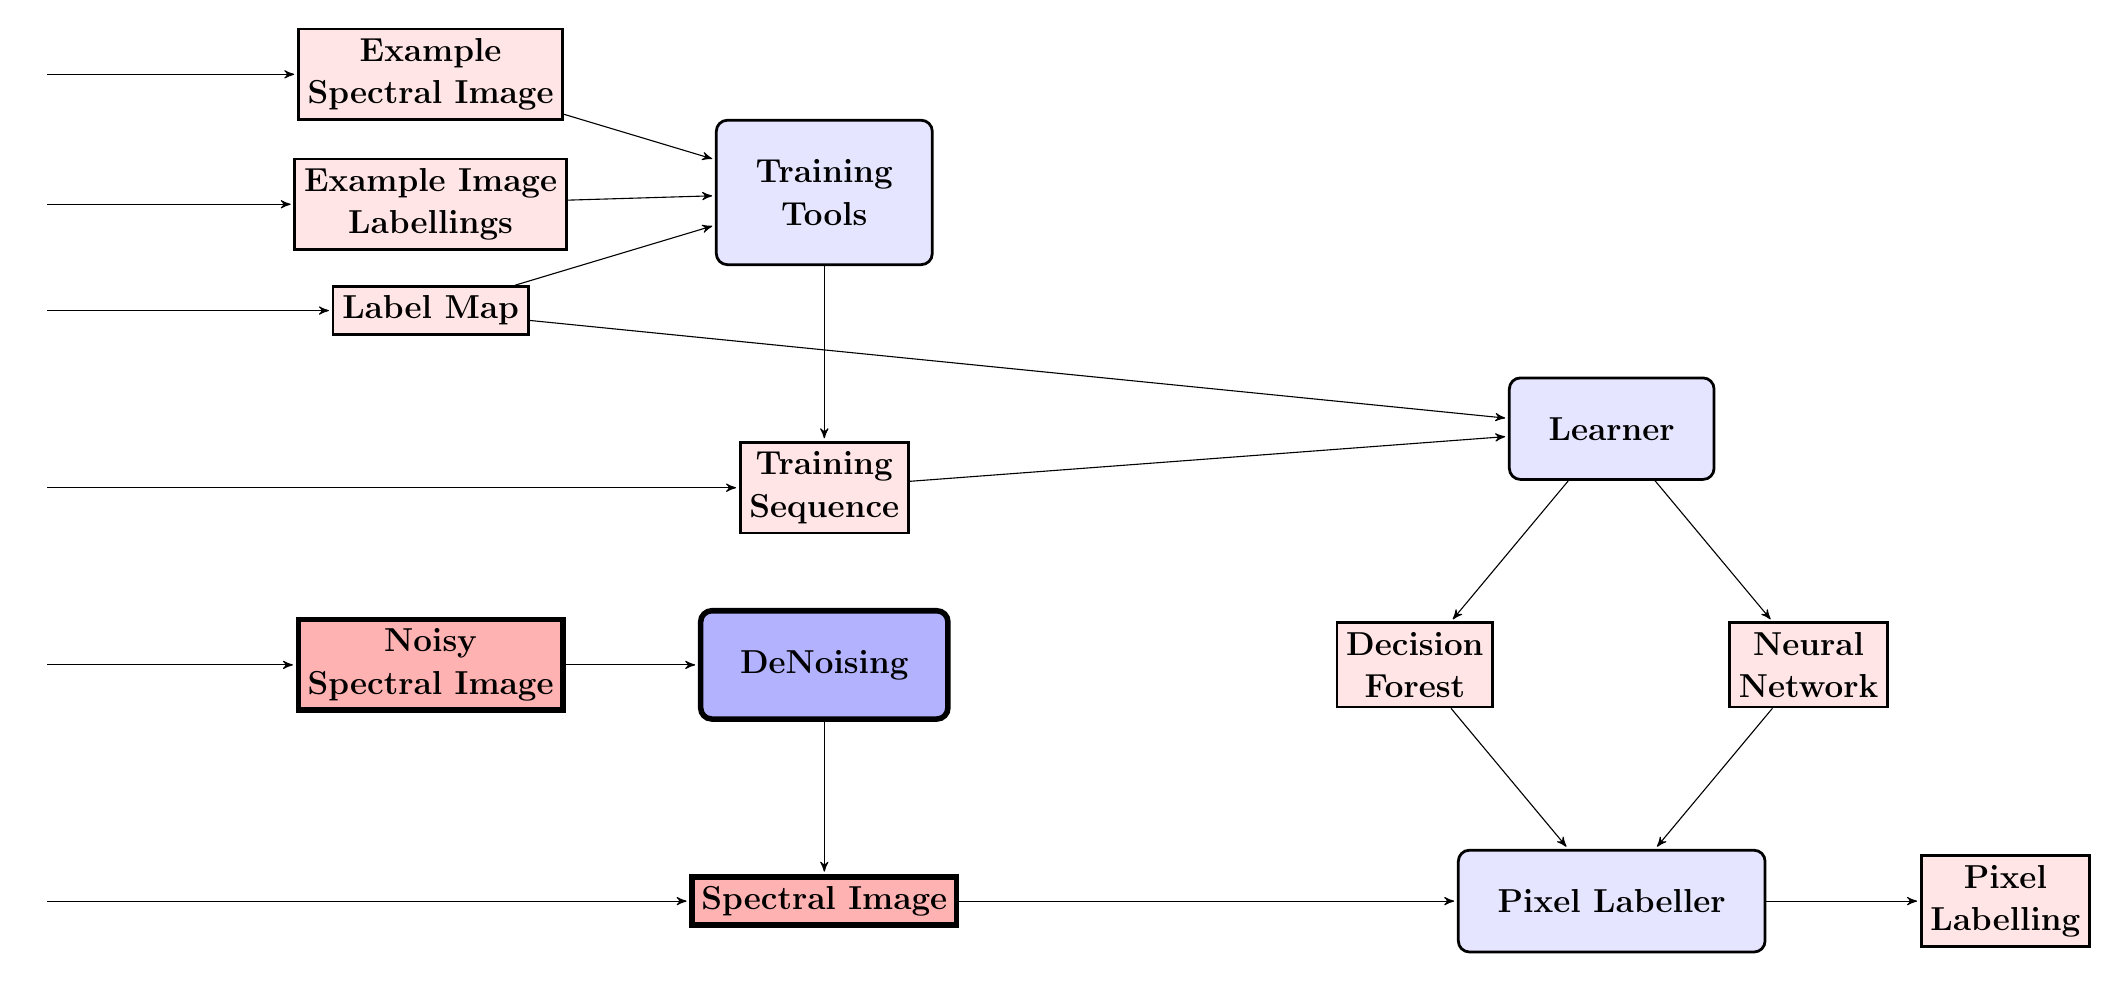
\begin{tikzpicture}[node distance=2cm,>=stealth',bend angle=45,auto]

                                \tikzstyle{commonNode}=[thick, font=\ttfamily\large\bf, align=center, line width=2pt, draw=black]
                                \tikzstyle{module}=[commonNode, rectangle, rounded corners, fill=blue!30, inner sep=5mm]
                                \tikzstyle{file}=[commonNode, fill=red!30]
                                \tikzstyle{unusedModule}=[module, fill=blue!10, line width=1pt]
                                \tikzstyle{unusedFile}=[file, fill=red!10, line width=1pt]
                                \tikzstyle{intermediateFile}=[file, dash pattern=on 3pt off 3pt, line width=1pt]

                                \begin{scope}
                                    % Spacing the nodes out
                                    \def \hspacing {5}
                                    \def \vspacing {3}
                                    \def \indent {0.25}

                                    % Background
                                    %\fill[black!20, rounded corners=10] (-0.75*\hspacing, 0.5*\vspacing) rectangle (4.5*\hspacing, 5.5*\vspacing);

                                    % Title
                                    %\node at (-0.75*\hspacing+\indent, 5.5*\vspacing-\indent) [anchor=north west] {\textbf{System Overview}};

                                    % Inputs
                                    \node at (-1*\hspacing, 4.5*\vspacing) (EHIin) {};
                                    \node at (-1*\hspacing, 3.95*\vspacing) (EILin) {};
                                    \node at (-1*\hspacing, 3.5*\vspacing) (LMin) {};
                                    \node at (-1*\hspacing, 2.75*\vspacing) (TSin) {};
                                    \node at (-1*\hspacing, 2*\vspacing) (NHIin) {};
                                    \node at (-1*\hspacing, 1*\vspacing) (HIin) {};

                                    % Files and modules
                                    \node at (0*\hspacing, 4.5*\vspacing) [unusedFile]    (EHI)     {Example \\ Spectral Image}
                                        edge  [pre]   (EHIin);
                                    \node at (0*\hspacing, 3.95*\vspacing)   [unusedFile]    (EIL)     {Example Image \\ Labellings}
                                        edge  [pre]   (EILin);
                                    \node at (0*\hspacing, 3.5*\vspacing) [unusedFile]    (LM)      {Label Map}
                                        edge  [pre]   (LMin);
                                    \node at (1*\hspacing, 4*\vspacing)   [unusedModule]  (TT)      {Training \\ Tools}
                                        edge  [pre]   (EHI)
                                        edge  [pre]   (EIL)
                                        edge  [pre]   (LM);
                                    \node at (1*\hspacing, 2.75*\vspacing)   [unusedFile]    (TS)      {Training \\ Sequence}
                                        edge  [pre]   (TSin)
                                        edge  [pre]   (TT);
                                    \node at (3*\hspacing, 3*\vspacing)   [unusedModule]  (L)       {Learner}
                                        edge  [pre]   (LM)
                                        edge  [pre]   (TS);
                                    \node at (2.5*\hspacing, 2*\vspacing) [unusedFile]    (F)       {Decision \\ Forest}
                                        edge  [pre]   (L);
                                    \node at (3.5*\hspacing, 2*\vspacing) [unusedFile]    (NN)      {Neural \\ Network}
                                        edge  [pre]   (L);
                                    \node at (0*\hspacing, 2*\vspacing)   [file]    (NHI)     {Noisy \\ Spectral Image}
                                        edge  [pre]   (NHIin);
                                    \node at (1*\hspacing, 2*\vspacing)   [module]  (DB)      {DeNoising}
                                        edge  [pre]   (NHI);
                                    \node at (1*\hspacing, 1*\vspacing)   [file]    (HI)      {Spectral Image}
                                        edge  [pre]   (HIin)
                                        edge  [pre]   (DB);
                                    \node at (3*\hspacing, 1*\vspacing)   [unusedModule]  (C)       {Pixel Labeller}
                                        edge  [pre]   (F)
                                        edge  [pre]   (NN)
                                        edge  [pre]   (HI);
                                    \node at (4*\hspacing, 1*\vspacing)   [unusedFile]    (PL)      {Pixel \\ Labelling}
                                        edge  [pre]   (C);
                                \end{scope}

                                % \begin{pgfonlayer}{background}
                                    
                                % \end{pgfonlayer}
                            \end{tikzpicture}
                        }

                    \caption{Overview of the de-noiser function.}
                \end{figure} 




            \subsubsection{Noisy Pixel Labeller}
                The noisy pixel labeller is a composite of the de-noiser and pixel labeller functions. We take a noisy 
                spectral image as input, along with a trained forest or neural network. De-noising is run on the image 
                before feeding the spectral image to the pixel labeller.

                \begin{figure}[H]
                    \centering
                        \scalebox{0.55}{ 
                            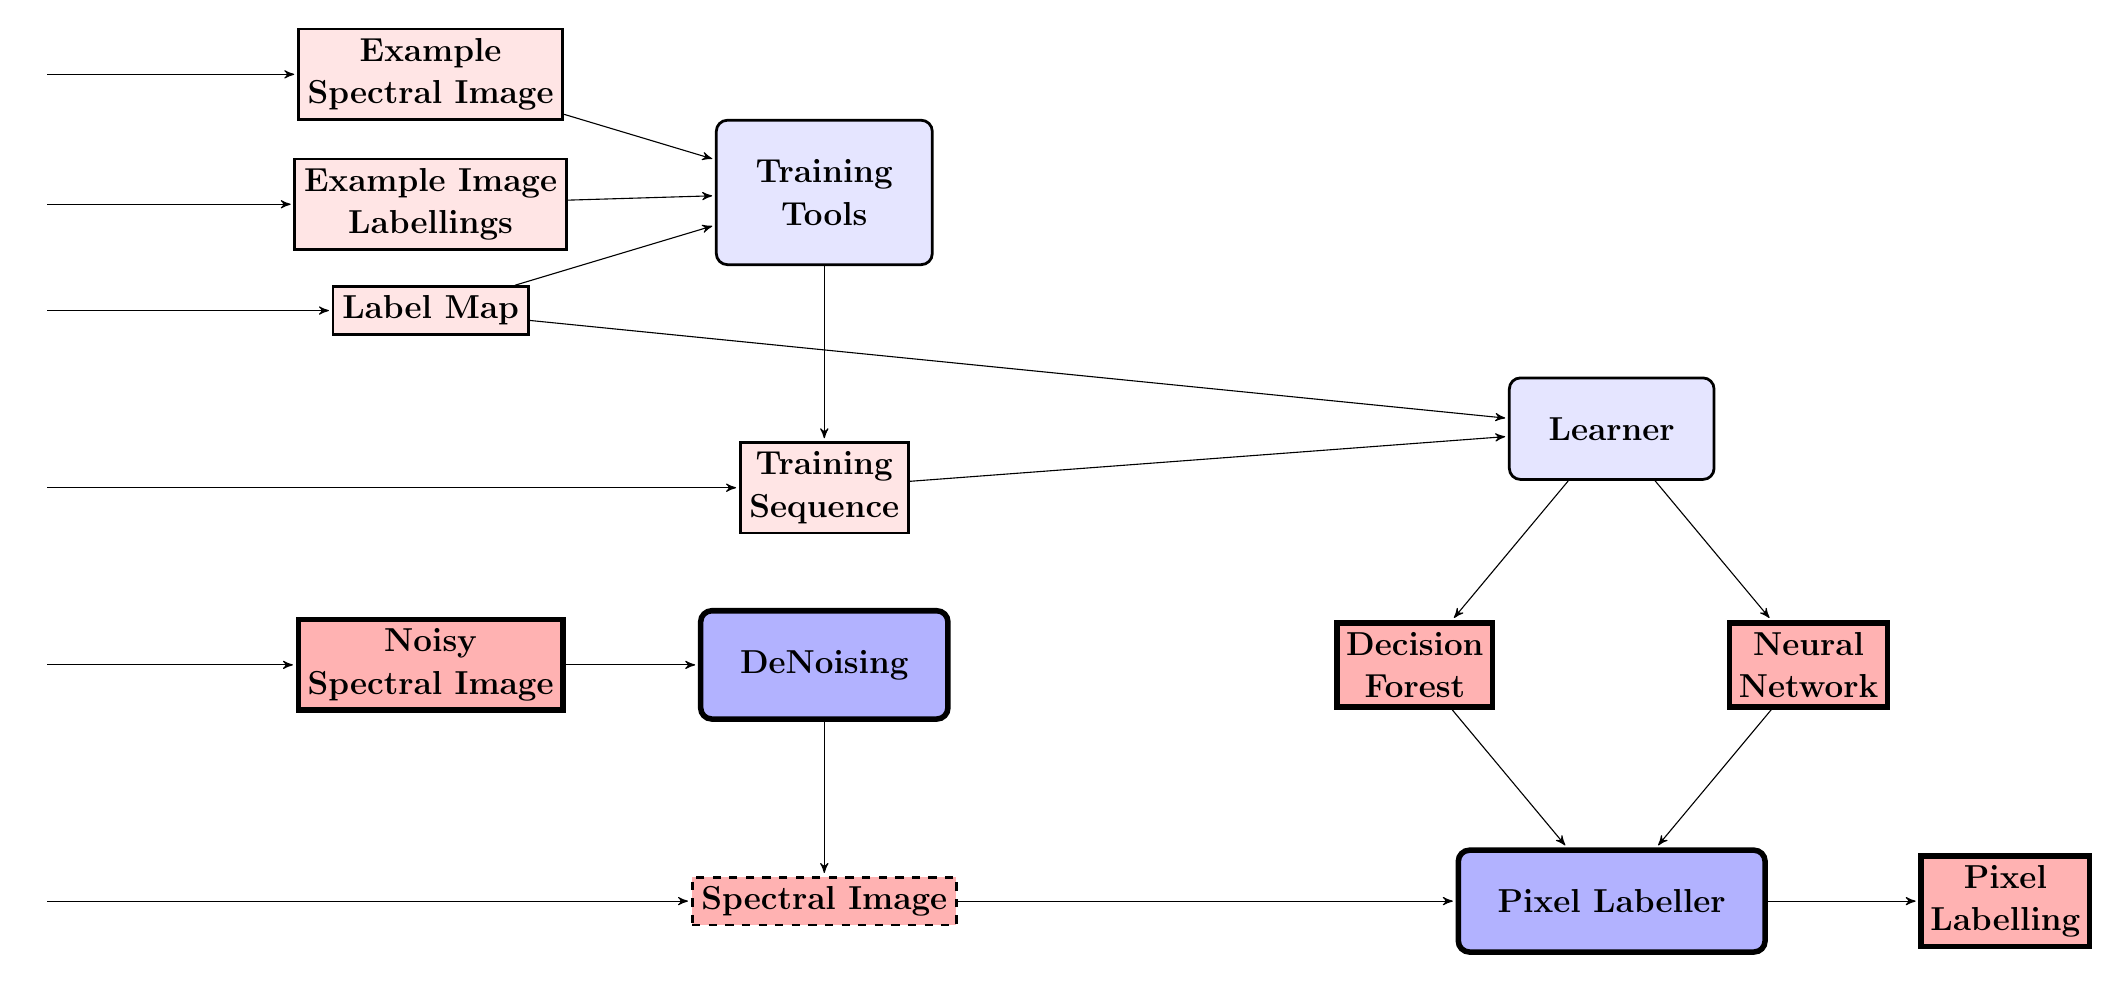
\begin{tikzpicture}[node distance=2cm,>=stealth',bend angle=45,auto]

                                \tikzstyle{commonNode}=[thick, font=\ttfamily\large\bf, align=center, line width=2pt, draw=black]
                                \tikzstyle{module}=[commonNode, rectangle, rounded corners, fill=blue!30, inner sep=5mm]
                                \tikzstyle{file}=[commonNode, fill=red!30]
                                \tikzstyle{unusedModule}=[module, fill=blue!10, line width=1pt]
                                \tikzstyle{unusedFile}=[file, fill=red!10, line width=1pt]
                                \tikzstyle{intermediateFile}=[file, dash pattern=on 3pt off 3pt, line width=1pt]

                                \begin{scope}
                                    % Spacing the nodes out
                                    \def \hspacing {5}
                                    \def \vspacing {3}
                                    \def \indent {0.25}

                                    % Background
                                    %\fill[black!20, rounded corners=10] (-0.75*\hspacing, 0.5*\vspacing) rectangle (4.5*\hspacing, 5.5*\vspacing);

                                    % Title
                                    %\node at (-0.75*\hspacing+\indent, 5.5*\vspacing-\indent) [anchor=north west] {\textbf{System Overview}};

                                    % Inputs
                                    \node at (-1*\hspacing, 4.5*\vspacing) (EHIin) {};
                                    \node at (-1*\hspacing, 3.95*\vspacing) (EILin) {};
                                    \node at (-1*\hspacing, 3.5*\vspacing) (LMin) {};
                                    \node at (-1*\hspacing, 2.75*\vspacing) (TSin) {};
                                    \node at (-1*\hspacing, 2*\vspacing) (NHIin) {};
                                    \node at (-1*\hspacing, 1*\vspacing) (HIin) {};

                                    % Files and modules
                                    \node at (0*\hspacing, 4.5*\vspacing) [unusedFile]    (EHI)     {Example \\ Spectral Image}
                                        edge  [pre]   (EHIin);
                                    \node at (0*\hspacing, 3.95*\vspacing)   [unusedFile]    (EIL)     {Example Image \\ Labellings}
                                        edge  [pre]   (EILin);
                                    \node at (0*\hspacing, 3.5*\vspacing) [unusedFile]    (LM)      {Label Map}
                                        edge  [pre]   (LMin);
                                    \node at (1*\hspacing, 4*\vspacing)   [unusedModule]  (TT)      {Training \\ Tools}
                                        edge  [pre]   (EHI)
                                        edge  [pre]   (EIL)
                                        edge  [pre]   (LM);
                                    \node at (1*\hspacing, 2.75*\vspacing)   [unusedFile]    (TS)      {Training \\ Sequence}
                                        edge  [pre]   (TSin)
                                        edge  [pre]   (TT);
                                    \node at (3*\hspacing, 3*\vspacing)   [unusedModule]  (L)       {Learner}
                                        edge  [pre]   (LM)
                                        edge  [pre]   (TS);
                                    \node at (2.5*\hspacing, 2*\vspacing) [file]    (F)       {Decision \\ Forest}
                                        edge  [pre]   (L);
                                    \node at (3.5*\hspacing, 2*\vspacing) [file]    (NN)      {Neural \\ Network}
                                        edge  [pre]   (L);
                                    \node at (0*\hspacing, 2*\vspacing)   [file]    (NHI)     {Noisy \\ Spectral Image}
                                        edge  [pre]   (NHIin);
                                    \node at (1*\hspacing, 2*\vspacing)   [module]  (DB)      {DeNoising}
                                        edge  [pre]   (NHI);
                                    \node at (1*\hspacing, 1*\vspacing)   [intermediateFile]    (HI)      {Spectral Image}
                                        edge  [pre]   (HIin)
                                        edge  [pre]   (DB);
                                    \node at (3*\hspacing, 1*\vspacing)   [module]  (C)       {Pixel Labeller}
                                        edge  [pre]   (F)
                                        edge  [pre]   (NN)
                                        edge  [pre]   (HI);
                                    \node at (4*\hspacing, 1*\vspacing)   [file]    (PL)      {Pixel \\ Labelling}
                                        edge  [pre]   (C);
                                \end{scope}

                                % \begin{pgfonlayer}{background}
                                    
                                % \end{pgfonlayer}
                            \end{tikzpicture}
                        }

                    \caption{Overview of the noisy pixel labeller function.}
                \end{figure} 







    \section{Languages and tools}
        In this section we briefly describe the languages, libraries and tools that we used for the project. \\

        \noindent\textbf{Programming Languages and Libraries}
            \begin{description}[font=\normalfont\itshape, labelindent=10pt]
                \item[Java:] provides an OS independent language and is object oriented to allow for modular design.
                \item[JUnit:] a Java library used for unit testing, used for white box and black box testing throughout 
                    the development of the system. Unit tests are essential to find bugs and prevent their re-introduction.
                \item[Encog:] an easy to use neural networks library in Java/C\# written by Heaton research \cite{JMLR:v16:heaton15a}. 
            \end{description}

        \noindent\textbf{Integrated development environment}
            \begin{description}[font=\normalfont\itshape, labelindent=10pt]
                \item[Eclipse:] allows for rapid development in Java and integrates easily with libraries and tools such 
                    as JUnit and Git.
                \item[EclEmma:] an Eclipse plug-in compatible with JUnit which highlights lines to indicate code coverage 
                    of unit tests.
                \item[ObjectAid:] another Eclipse plug-in, used to create UML class diagrams.
            \end{description}

        \noindent\textbf{Statistical analysis and visualisation}
            \begin{description}[font=\normalfont\itshape, labelindent=10pt]
                \item[Matlab:] an easy to use, extensible statistical package used for producing graphs.
            \end{description}

        \noindent\textbf{Document preparation}
            \begin{description}[font=\normalfont\itshape, labelindent=10pt]
                \item[\LaTeX:] used for typesetting this dissertation in a precise manor allowing control over most 
                    aspects of document layout and style.
                \item[Tikz:] a \LaTeX\ library useful for producing diagrams, such as Figure \ref{fig:system_overview}.
                \item[Listings:] a \LaTeX\ library allowing colour formatted code for a plethora of languages.
                \item[Adobe Photoshop:] image editing software used to produce some diagrams.
            \end{description}

        \noindent\textbf{Version Control}
            \begin{description}[font=\normalfont\itshape, labelindent=10pt]
                \item[Git:] allows code to be developed systematically and rollback if necessary, as well as providing  
                    the ability to fork my core repository to try different strategies.
            \end{description}

        \noindent\textbf{Backup}
            \begin{description}[font=\normalfont\itshape, labelindent=10pt]
                \item[DropBox and Google Drive:] repositories were kept in both DropBox and Google Drive folders, which 
                    synced every time a file was changed.
                \item[Github:] provides a remote Git repository to store code, so also helps in provision of version 
                    control. The repository was updated every time a stable commit was made.
                \item[Time machine:] Apple's automatic backup system, allowing for hourly backups of the whole hard drive 
                    to be taken.
            \end{description}



    \section{Software engineering techniques}
        \subsection{Development model}
            The design of the system calls for a mixture of iterative and waterfall models to be employed in this project.
            The system is split into well defined modules (as can be seen in Figure \ref{fig:system_overview}). Each module 
            then needs to be implemented and tested rigorously before moving onto the next, important because of the 
            dependencies between modules. For each module it is possible to produce manually suitable files for testing.

            Once a working system was produced, tested and deemed to be correct with some confidence, additional 
            features and improvements to the system were added in an iterative manner, similar to a spiral model. Unit 
            tests were used to make sure that any new additions do not break the existing, working parts of the system.

        \subsection{Testing}
            Development was test driven by necessity, as a large amount of work was required to reach a 
            \textit{minimum viable product}. If it were not tested thoroughly throughout development could have lead 
            to nasty and difficult to find bugs. All tests were written as unit tests so that 
            they could be reused later to make sure that the system still works.
            The following methodologies were employed:
            \begin{description}[font=\normalfont\itshape, labelindent=10pt]
                \item[Black box testing:] When the internal system design is not taken into account, black box testing is 
                    used to ensure that the system works as a `black box', in terms of the expected 
                    input/outputs we specified in the design. To assure that internal system design wasn't taken 
                    into account these were written \textit{before} any code was written.
                \item[White box testing:] When the internal system design is taken into account, tests are designed so that every 
                    line of code is checked using the unit tests. This is difficult to check manually, so Eclipse plug-in 
                    EclEmma was used, a code coverage tool that works with JUnit.
                \item[Input sanitisation testing:] Additional unit tests were written to make sure that erroneous inputs 
                    were handled correctly.
                \item[Incremental integration testing:] This refers to using a bottom up approach, testing functionality 
                    as it is implemented.
                \item[Usability testing:] A few users were asked to try use the system given only instructions in a readme 
                    file. The feedback was vital in shaping the design of the training tools module.
            \end{description}

        \subsection{Backup Plan}
            It is important to make sure that we have an effective backup plan to avoid any software, hardware or 
            user error that may result in a loss of work, which is important to ensure that we do not 
            lose a year's worth of work. 

            To make sure that no work was lost a number of systems were set in place to not only regularly back up 
            any work but also provide rollback if necessary. Google Drive and DropBox were employed to keep shadow 
            copies of the project directory, GitHub was used as a remote repository which was pushed to regularly. 
            Finally Apple's time machine software was also used to automatically take backups of the whole local 
            file system every hour.

            \begin{figure}
                \centering
                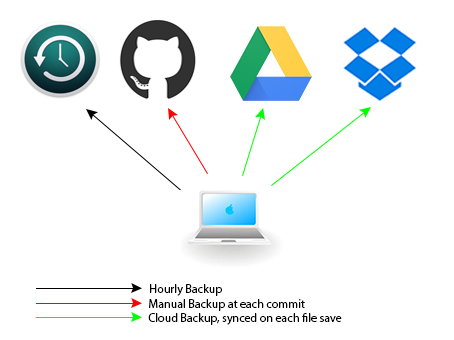
\includegraphics[scale=0.75]{backup_plan}
                \caption[Overview of the backup strategy employed.]{Overview of the backup strategy employed\footnotemark.}
            \end{figure}
            \footnotetext{Image modified from: 
                \href{http://www.apple.com/airport-time-capsule/}{apple.com}, 
                \href{https://www.google.com/drive/}{google.com}, 
                \href{https://www.dropbox.com/business/why-dropbox-for-business}{dropbox.com}, 
                \href{https://github.com/}{github.com}, 
                \href{http://www.clipartpanda.com/categories/mac-computer-clip-art}{clipartpanda.com}.}





%%%%%%%%%%%%%%%%%%%%%%%%%%%%%%%%%%%%%%%%%%%%%%%%%%%%%%%%%%%%%%%%%%%%%%%%%%%%%%%%%%%%%%%%%%%%%%%%%%%%%%%%%%%%%%%%%%%%%%%%
% the implementation

\cleardoublepage
\chapter{Implementation}
    This chapter by elaborates on the implementation of the Random Forests algorithm and the use of the Encog, a 
    neural network library for Java. We then proceed to use the supervised learning methods to build a procedure for 
    producing a pixel labelling from a spectral image. We initially set aside the problems of how we will produce 
    training data for the supervised learning methods, as these likely need to be extracted from an example labelling, 
    a problem that will be addressed in section \ref{sec:training_tools}, along with the treatment of image noise in 
    section \ref{sec:de-noising}.

    The project is modularised into a number of packages, each building on top of another. Dependencies can be 
    visualised in Figure \ref{fig:package_dependencies}. We will use UML class 
    diagrams\footnote{As defined in http://www.uml-diagrams.org/class-reference.html} 
    to show the overview of classes within each package.

    \begin{framed}
        Add dependency from NN to RF because of use of ProbabilityDistribution class
    \end{framed}

    \begin{figure}[H]
        \centering
        \scalebox{0.55}{ 
            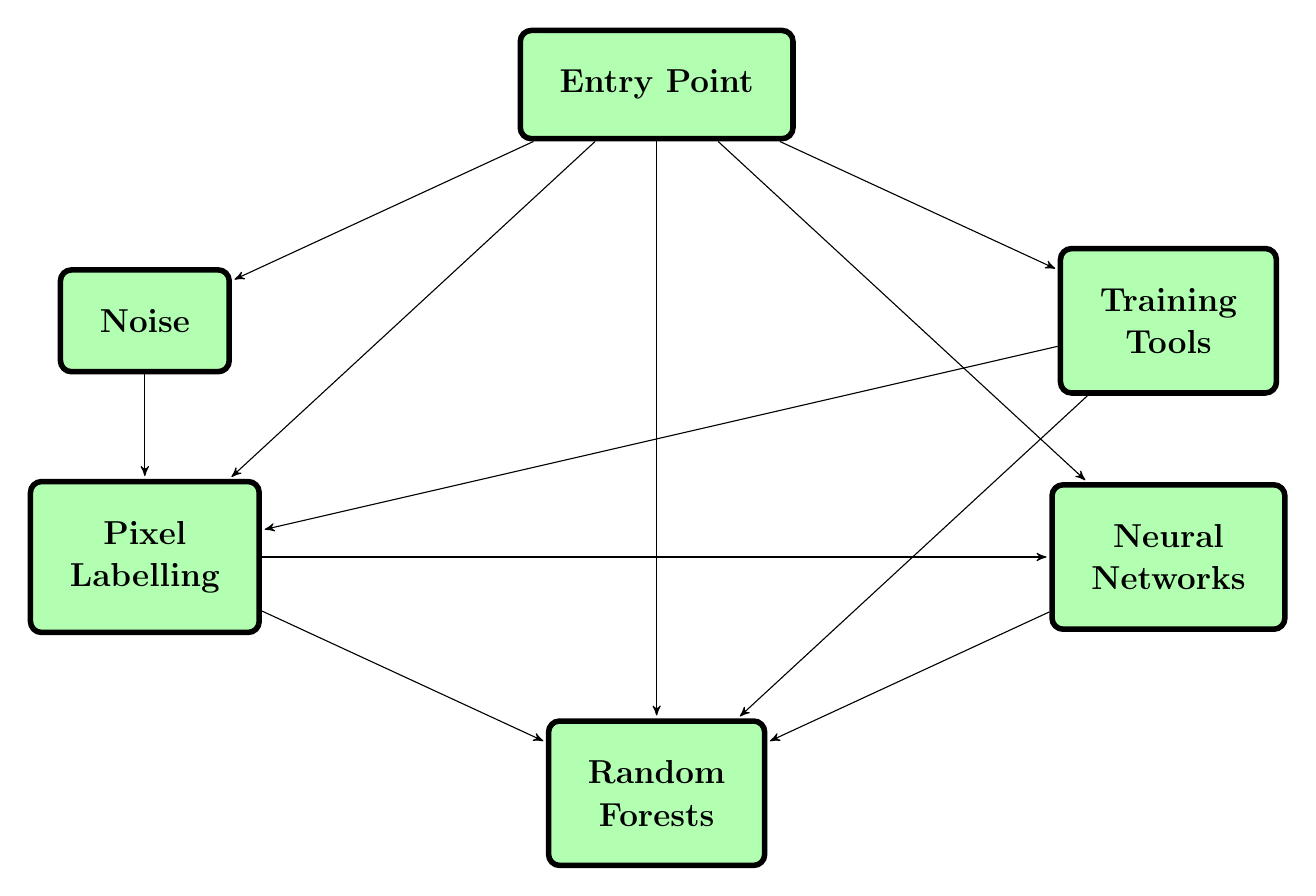
\begin{tikzpicture}[node distance=2cm,>=stealth',bend angle=45,auto]

                \tikzstyle{commonNode}=[thick, font=\ttfamily\large\bf, align=center, line width=2pt, draw=black]
                \tikzstyle{package}=[commonNode, rectangle, rounded corners, fill=green!30, inner sep=5mm]

                \begin{scope}

                    \def \hspacing {5}
                    \def \vspacing {3}

                    % Files and modules
                    \node at (2*\hspacing, 3*\vspacing) [package] (EP) {Entry Point};
                    \node at (3.3*\hspacing, 2*\vspacing) [package] (TT) {Training \\ Tools}
                        edge  [pre] (EP);
                    \node at (0.7*\hspacing, 2*\vspacing) [package] (N) {Noise}
                        edge  [pre] (EP);
                    \node at (0.7*\hspacing, 1*\vspacing) [package]  (PL) {Pixel \\ Labelling}
                        edge  [pre] (EP)
                        edge  [pre] (TT)
                        edge  [pre] (N);
                    \node at (3.3*\hspacing, 1*\vspacing) [package] (NN) {Neural \\ Networks}
                        edge  [pre] (PL)
                        edge  [pre] (EP);
                    \node at (2*\hspacing, 0*\vspacing) [package] (RF)  {Random \\ Forests}
                        edge  [pre] (EP)
                        edge  [pre] (TT)
                        edge  [pre] (PL)
                        edge  [pre] (NN);
                \end{scope}
            \end{tikzpicture}
        }


        \caption[The dependencies between different packages/modules defined in the system.]{The dependencies between different packages/modules defined in the system. An arrow from A to B means that package A depends on package B. 
        Although the TrainingTools package produces training files for both NeuralNetworks and RandomDecisionForests, it only
        \textit{depends} on RandomDecisionForests as it uses the class \texttt{TrainingSequence}. EntryPoint is the package used to define the interface to the whole system, and provides the \texttt{main} file for the eventual \texttt{.jar}.}
        \label{fig:package_dependencies}
    \end{figure}




    \section{Random Forests Library}
        We begin by describing our implementation of random forests, looking specifically at critical design 
        choices that were made. A generic and easily extensible random forests library is implemented, which can 
        be specialised for many applications, then specialising subclasses are written that utilise the library for our 
        purpose of providing a pixel labelling.

        \begin{figure}[H]
            \centering
            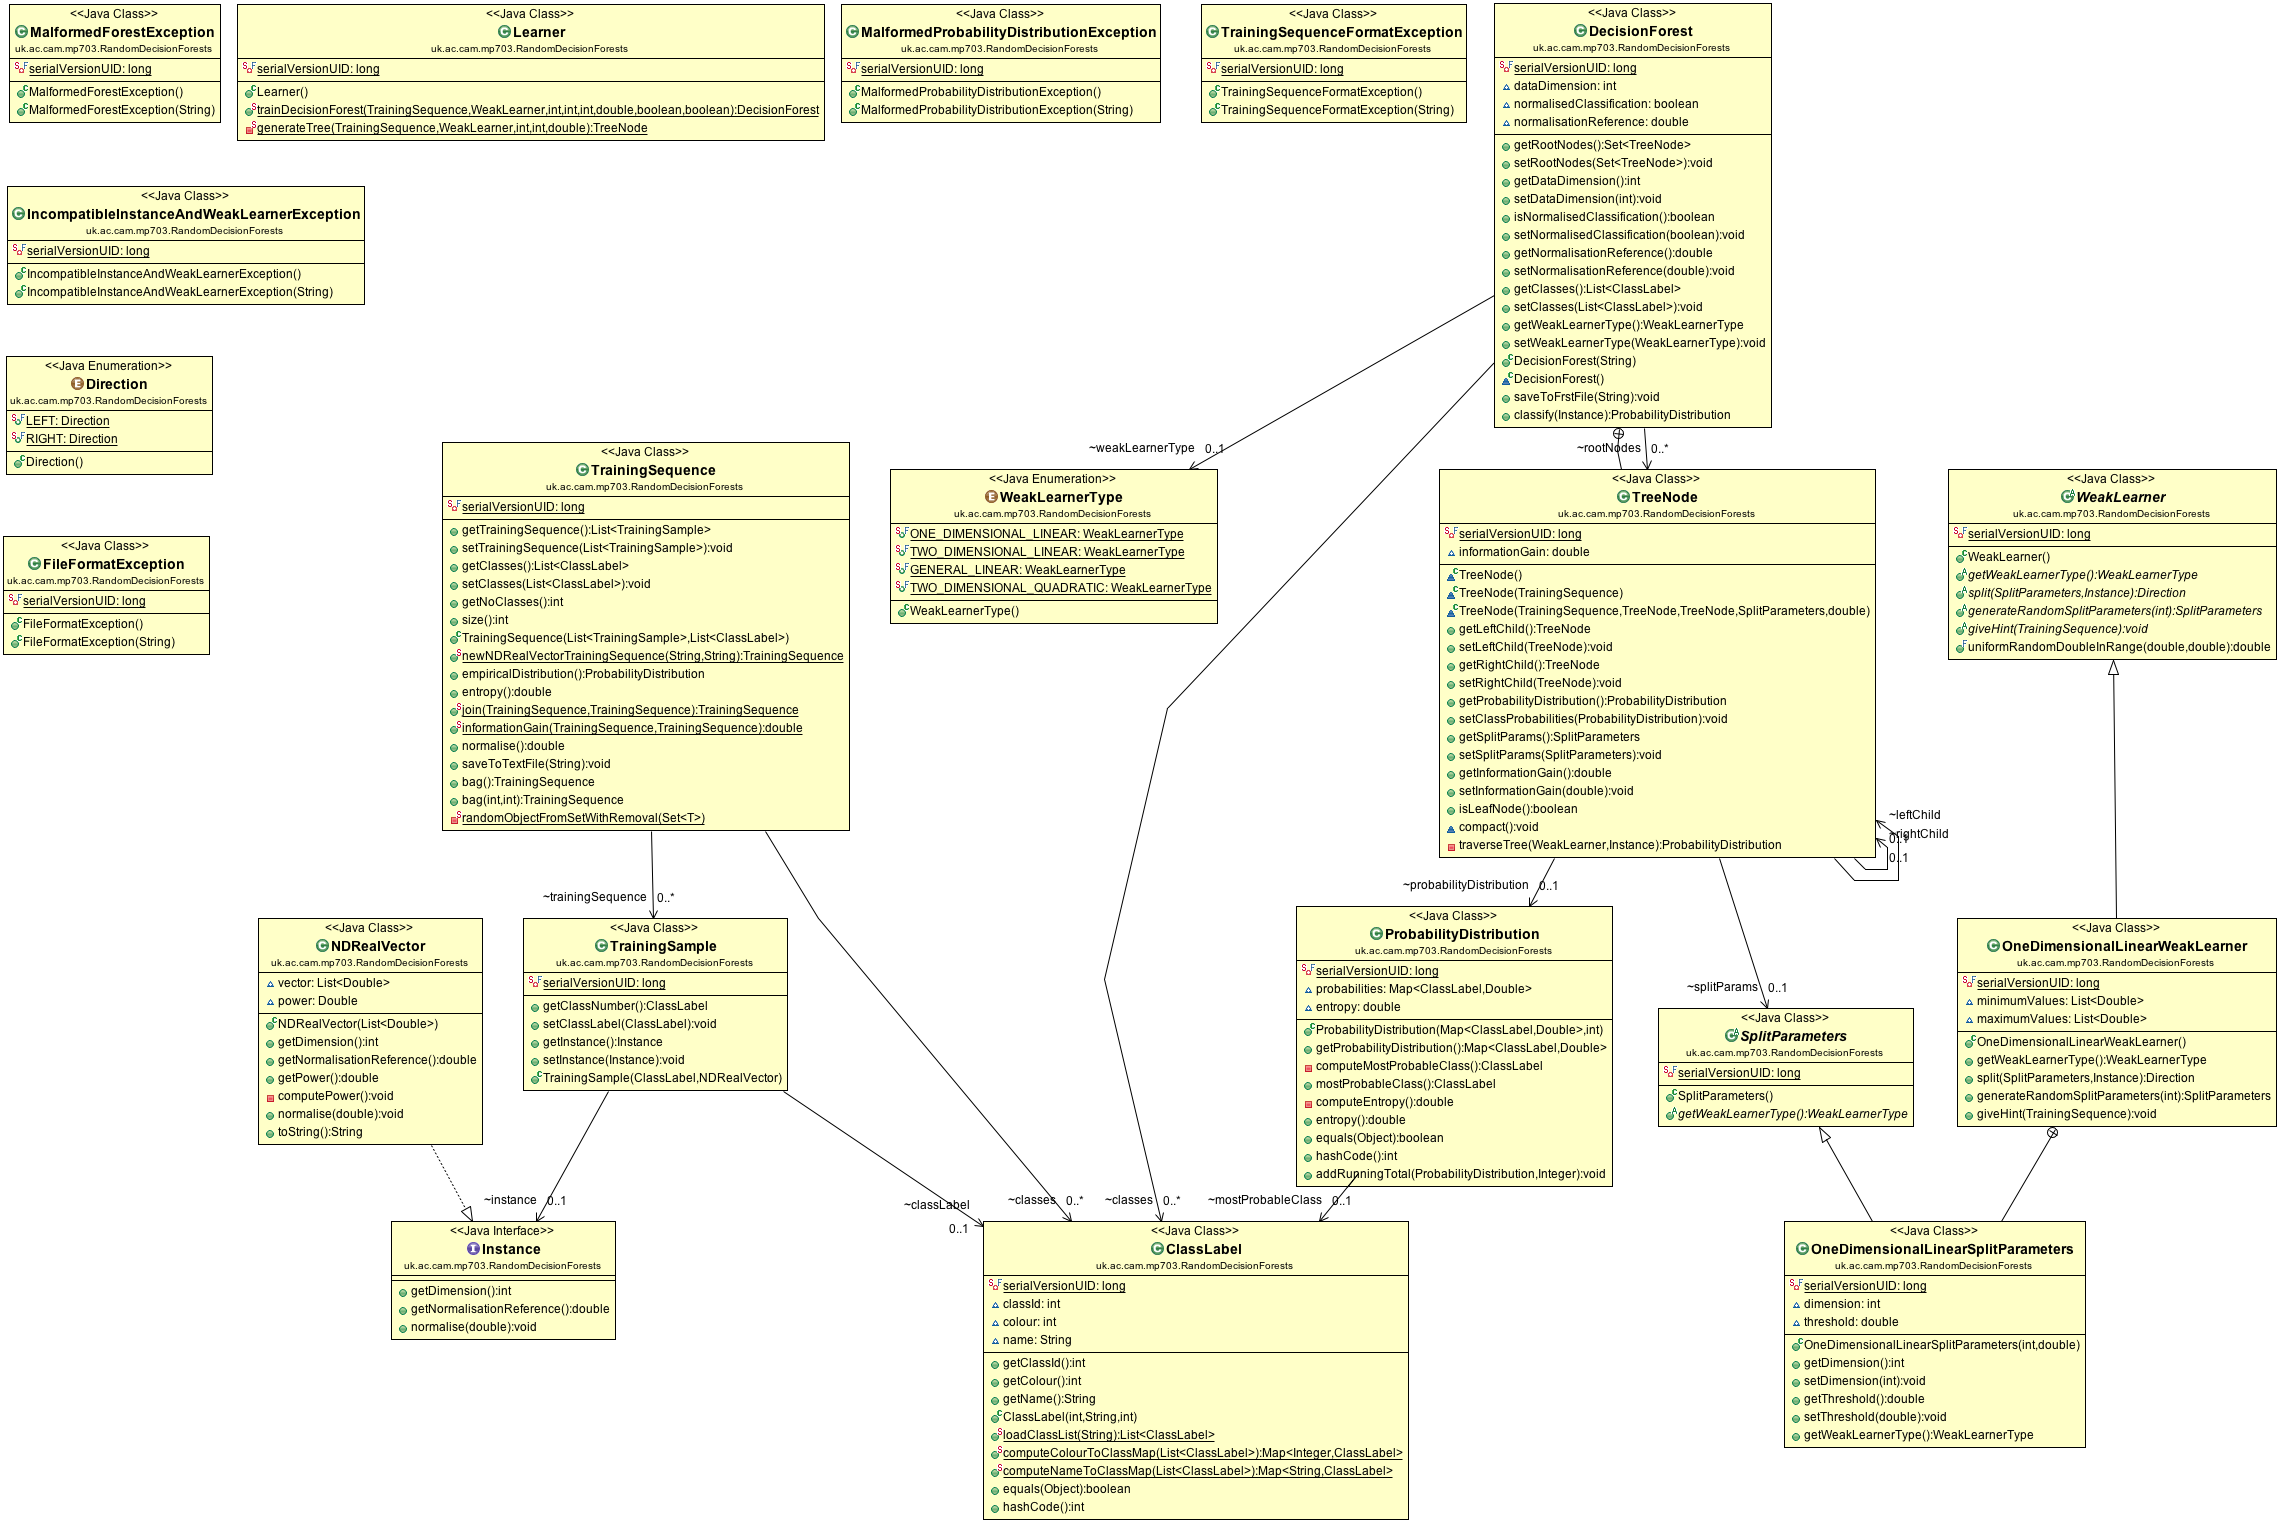
\includegraphics[scale=0.25, angle=90]{Forest_UML}
            \caption[An overview of classes in the RandomDecisionForest package]{An overview of classes in the RandomDecisionForest package, from which relevant sections will be 
            looked at closer when appropriate.}
            \label{fig:forest_uml}
        \end{figure}

        \subsection{Data structures}
            A number of important data structures are used throughout the library, each requiring an efficient 
            implementation and providing necessary abstraction. Before we move onto the more complicated issues 
            regarding supervised learning, we need to describe the structures used. This subsection 
            describes the main classes that are used in the RandomDecisionForest package, providing a table of 
            functions defined with corresponding English descriptions of what they do and some small code listings 
            where necessary.



            \subsubsection{ClassLabels}
                Our first class, \texttt{ClassLabels}, abstracts classification labels into its own class. As can be 
                seen in Figure \ref{fig:class_label_uml} \texttt{ClassLabels} groups together a class name and its 
                corresponding colour, both of which should be unique, and we note that \texttt{classId} is only used 
                internally. The colour will be used sections 
                \ref{sec:pixel_label} and \ref{sec:training_tools} to indicate its corresponding class in a pixel 
                labelling, where the pixel labelling is either input in a ``ground truth'' image or output by our system.                

                \begin{figure}[H]
                    \centering
                    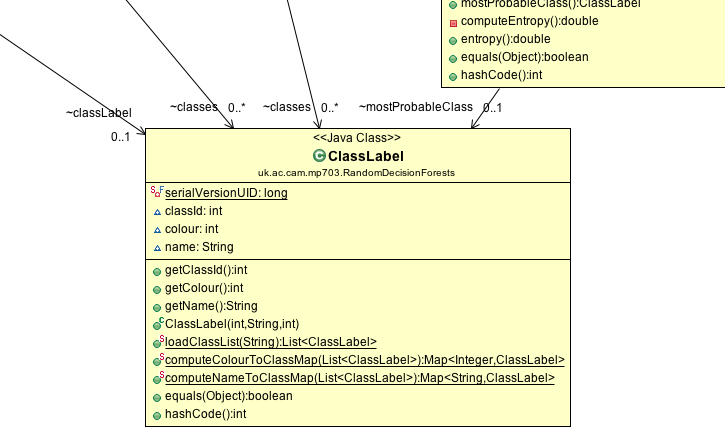
\includegraphics[scale=0.5]{ClassLabel_Forest_UML}
                    \caption[A closer view of \texttt{ClassLabel}]{A closer view of \texttt{ClassLabel} in Figure \ref{fig:forest_uml}.}
                    \label{fig:class_label_uml}
                \end{figure}

                \begin{table}[H]
                    \begin{tabularx}{\textwidth}{l|X}
                        \textbf{Function Name} & \textbf{Function Description} \\
                        \hline

                        \texttt{loadClassList} & 
                            A \texttt{static} function that returns a value of type \texttt{List<ClassLabel>} given a 
                            filename specifying ``class colour map'' as in appendix \ref{app:file_formats}, of classes 
                            specified in the file. In this function we make sure that we preserve the uniqueness of 
                            class names their associated colours. \\
                        \hline

                        \texttt{computeColourToClassMap} & 
                            Returns a value of type \texttt{Map<Integer, ClassLabel>}, a mapping from a class colours to 
                            their corresponding \texttt{ClassLabel} objects. \\ 
                        \hline

                        \texttt{computeNameToClassMap} & 
                            Returns a value of type \texttt{Map<String, ClassLabel>}, a mapping from a class names to 
                            their corresponding \texttt{ClassLabel} objects. \\
                        \hline

                        \texttt{equals} &
                            An override of \texttt{Object}'s equality function. This is needed as we will frequently 
                            use \texttt{ClassLabel} as the key to a map structure, and might not use the same instance 
                            as a key. The function checks that the class name's, class colour's and class id's are 
                            identical. \\
                        \hline

                        \texttt{hashCode} &
                            Similarly to \texttt{equals} this is overridden for a correct implementation when 
                            \texttt{ClassLabel} is used as the key in a (hash) map structure.

                    \end{tabularx}
                    \caption{Important methods implemented in the \texttt{ClassLabel} class.}
                    \label{tab:ClassLabel}
                \end{table}




            \subsubsection{Instances}
                The \texttt{Instance} class is used to specify a feature vector, or some instance of our problem. We 
                define an interface to represent the base structure of an instance. 

                \begin{figure}[H]
                    \centering
                    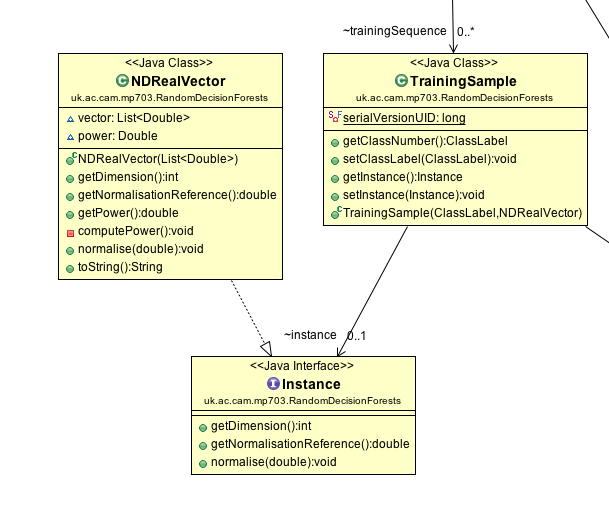
\includegraphics[scale=0.5]{Instance_Forest_UML}
                    \caption{A closer view of \texttt{Instance} in Figure \ref{fig:forest_uml}.}
                    \label{fig:instance_uml}
                \end{figure}

                A feature vector will have some finite number of `features' that we use and the \texttt{getDimension} 
                function that should return the number of features (i.e. the dimension) in the instance. The functions 
                \texttt{getNormalisationReference} and \texttt{normalise} are used for normalisation of instances. 
                During classification we may want to normalise so that small changes in data with low variance have 
                the same weighting as larger changes in data with low variance. This is explored more in section 
                \ref{sec:effect_of_normalisation}. Intuitively we define some sort of `power' value for each instance 
                and use normalisation so that all \texttt{Instance}s have the same power. It is optional to use 
                normalisation in the learning (and therefore classification) algorithms in sections \ref{sec:training} 
                and \ref{sec:classification}. 

                Let \texttt{NDRealVector} be a concrete implementation of \texttt{Instance} which can also 
                be seen in Figure \ref{fig:instance_uml}. We use \texttt{NDRealVector} to represent spectra in spectral 
                images, that is, values in $\bb{R}^N$. We can simply think of this as 
                a wrapper for a list of values. We also store the power of the spectrum, and use this as our 
                ``normalisation reference'' value. The \textit{power} of a spectrum (or vector) is the sum 
                of squared values in the list.

                \begin{table}[H]
                    \begin{tabularx}{\textwidth}{l|X}
                        \textbf{Function Name} & \textbf{Function Description} \\
                        \hline

                        \texttt{getDimension} & 
                            This returns $n$ if there are $n$ values in \texttt{vector}, our list of doubles.  \\ 
                        \hline

                        \texttt{getPower} & 
                            This returns the power of the spectrum of values. If we consider the list of values 
                            to be $\vc{v}$ then we return $||\vc{v}||^2$. \\ 
                        \hline

                        \texttt{getNormalisationReference} & 
                            This function returns the power of the spectrum. \\
                        \hline

                        \texttt{normalise} & 
                            Normalisation of vectors can be implemented by scalar division of the vector with the power. 
                            I.e. we divide all values in the spectrum by the power. \\ 
                        \hline

                        \texttt{toString} & 
                            We override \texttt{Object}'s \texttt{toString} method. This is used later in section 
                            \ref{sec:training_tools} when we wish to print a training sequence to a text file. It 
                            simply returns a comma separated list of values. 

                    \end{tabularx}
                    \caption{Important methods implemented in the \texttt{NDRealVector} class.}
                    \label{tab:NDRealVector}
                \end{table}



            \subsubsection{Probability Distributions} \label{sec:prob_dist}
                As discussed in section \ref{sec:rand_forest} probability distributions are associated with each node, 
                and is the effective output from the classification algorithm. Thus any implementation of Random Forests 
                needs to have some way to represent probability distributions over possible classifications. Although 
                we can represent a probability distribution as \texttt{Map<ClassLabel, Double>}, we choose to 
                encapsulate this in its own class \texttt{ProbabilityDistribution} so that we can perform validation
                on the properties of a probability distribution, that is each probability is a value in $[0,1]$ and 
                the probabilities sum to a $1$ and we also cache some frequently used values such as \texttt{entropy}. 

                The \textit{entropy} of a probability distribution $p:\Omega\rightarrow[0,1]$ can be defined as:

                \begin{align}
                  H(p) = \sum\limits_{x\in\Omega} -p(x) \log_2(p(x))
                  \label{eq:prob_entropy}
                \end{align}

                which is consistent with the definition of entropy given in equation \ref{eq:training_seq_entropy}.

                \begin{figure}[H]
                    \centering
                    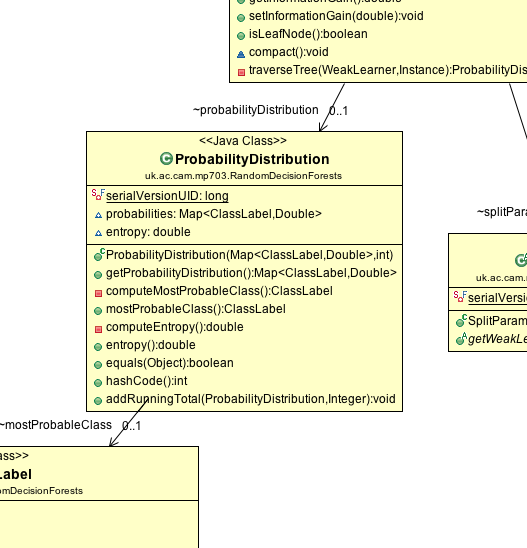
\includegraphics[scale=0.5]{ProbabilityDistribution_Forest_UML}
                    \caption{A closer view of \texttt{ProbabilityDistribution} in Figure \ref{fig:forest_uml}.}
                    \label{fig:prob_dist_uml}
                \end{figure}

                The class is immutable so that we cannot accidentally modify the distribution into something 
                invalid. Therefore we make each variable \texttt{final} and remove any setter functions. 
                We also make use of the \texttt{unmodifiableMap} function in the \texttt{Java.Collections} 
                package, when setting the \texttt{probabilities} variable. This gives a reference to a \texttt{Map} 
                where no entries can be added, nor removed, which prevents someone from getting a reference to the map
                \texttt{probabilities} and altering it.

                Also in the implementation of the class constructor we allow for a small error in the sum, this is 
                because we will often have small errors from rounding in floating point numbers. The checks that 
                are made in the constructor of \texttt{ProababilityDistribution} are:
                \begin{itemize}
                    \item 
                        each value is in the range $[0,1]$;
                    \item 
                        the sum of values is in the range $[1-\epsilon,1+\epsilon]$, for some $0 < \epsilon \ll 1$.
                \end{itemize}

                Another implementation problem is found in the computation of entropy, as $-y\log_2(y)$ isn't defined for 
                the value of $y=0$. Mathematically we solve this problem by setting

                \begin{align}
                    -y\log_2(y)|_{y=0} & \defeq \lim_{y\to 0} -y \log_2(u) \\
                        & = 0.
                \end{align}

                When computing entropy according to equation \ref{eq:prob_entropy} we try to sum with $p(x)=0$ for 
                some $x$. In this case we would accidentally set the sum to a \texttt{NaN} value

                \begin{align}
                  \texttt{sum} &= \texttt{sum} + 0.0 * \log(0.0) \\
                    &= \texttt{sum} + 0.0 * -\infty \\
                    &= \texttt{sum} + \texttt{NaN}\\
                    &= \texttt{NaN},
                \end{align}

                where $\infty$ is the floating point representation of infinity, and we have 

                \begin{align}
                  \log(0.0) &= -\infty, \\
                  0.0 * \infty &= \texttt{NaN}.  
                \end{align}

                in accordance with the IEEE 754 standard \cite{1985--ieee754}. We hence need to skip over updating the 
                accumulating \texttt{sum} variable when $p(x) = 0$ otherwise we will accidentally set \texttt{sum} to a 
                \texttt{NaN} value.

                When classifying a using a decision tree we need to take an average over many probability distributions. 
                Consider the problem of numerically computing an average
                \begin{align}
                    \overline{x}_n = \frac{1}{n} \sum\limits_{i=1}^n x_i.
                    \label{eq:sum}
                \end{align}

                Then a na\"{i}ve implementation would first compute the value of $\sum\limits_{i=1}^n x_i$ and then 
                divide by $n$, however for very large $n$ this can lead to numerical instability, introducing a large 
                rounding error. We know that the following relation holds 

                \begin{align}
                    \overline{x}_n = \overline{x}_{n-1} + \frac{x_n - \overline{x}_{n-1}}{n}
                    \label{eq:numstabsum}
                \end{align} 

                and is easily verified by substituting equation \ref{eq:sum} in the right hand side of equation 
                \ref{eq:numstabsum}. This can be used to compute $\overline{x}_n$ accurately for large $n$ and we 
                should provide a method to perform the equivalent procedure to equation \ref{eq:numstabsum} over 
                probability distributions.

                \begin{lstlisting}[float=tp,caption={[The \texttt{ProbabilityDistribution} constructor.] Part of the \texttt{ProbabilityDirstribution} constructor, where we set $\epsilon = 2^{-10}$.}]
public class ProbabilityDistribution implements Serializable {

  ...

  public ProbabilityDistribution(
    Map<ClassLabel, Double> distribution, int noClasses) 
      throws MalformedProbabilityDistributionException {
    
    ...
    
    // Check that the sum is 1, allowing for a small floating 
    // point error
    double eps = 1e-10;
    if (sum < 1.0-eps || 1.0+eps < sum) {
      throw new MalformedProbabilityDistributionException;
    }
    
    // Assign the values (so they are immutable)
    this.probabilities = 
      Collections.unmodifiableMap(distribution);
    this.mostProbableClass = computeMostProbableClass();
    this.entropy = computeEntropy();
  }

  ...
}
                \end{lstlisting}                


                \begin{table}[H]
                    \begin{tabularx}{\textwidth}{l|X}
                        \textbf{Function Name} & \textbf{Function Description} \\
                        \hline

                        \texttt{computeMostPorbableClass} & 
                            Returns the \texttt{ClassLabel} with the highest probability in the distribution. This 
                            function is labelled private and is only used in the constructor. \\ 
                        \hline

                        \texttt{mostProbableClass} & 
                            Getter for the \texttt{mostProbableClass} value. \\ 
                        \hline

                        \texttt{computeEntropy} & 
                            Computes the entropy and returns the value. This function is labelled private and is only 
                            used in the constructor. \\ 
                        \hline

                        \texttt{entropy} & 
                            Getter for the \texttt{entropy} value. \\ 
                        \hline

                        \texttt{equals} & 
                            Override of \texttt{Object}'s function \texttt{equals}, returns true if the variable 
                            \texttt{probabilities} are equal in the two objects. We want this when comparing 
                            probability distributions rather than referential equality. \\ 
                        \hline

                        \texttt{hashCode} & 
                            Override of \texttt{Object}'s function \texttt{equals}, as we have overridden the 
                            \texttt{equals} function. \\ 
                        \hline

                        \texttt{addRunningTotal} &
                            Add a probability to a running average distribution to avoid numerical instability problems 
                            as discussed above, using equation \ref{eq:numstabsum}.

                    \end{tabularx}
                    \caption[Important methods implemented in \texttt{ProbabilityDistribution}.]{Important methods implemented in the \texttt{ProbabilityDistribution} class.}
                    \label{tab:ProbabilityDistribution}
                \end{table}



            \subsubsection{Training Sequences}
                The \texttt{TrainingSample} object is a pairing between a \texttt{ClassLabel} and an 
                \texttt{Instance}. There are no other functions in this class other than the getters, setters and 
                constructor. 

                A \texttt{TrainingSequence} consists of a list of \texttt{TrainingSample}s, and we keep a list of 
                \texttt{ClassLabel}s for reference. A number of convenience functions are defined in the class and 
                are listed in table \ref{tab:TrainingSequence}, which are used to compute useful values, such as
                entropy and information gain from equations \ref{eq:training_seq_entropy} and \ref{eq:information_gain} 
                respectively.

                \begin{figure}[H]
                    \centering
                    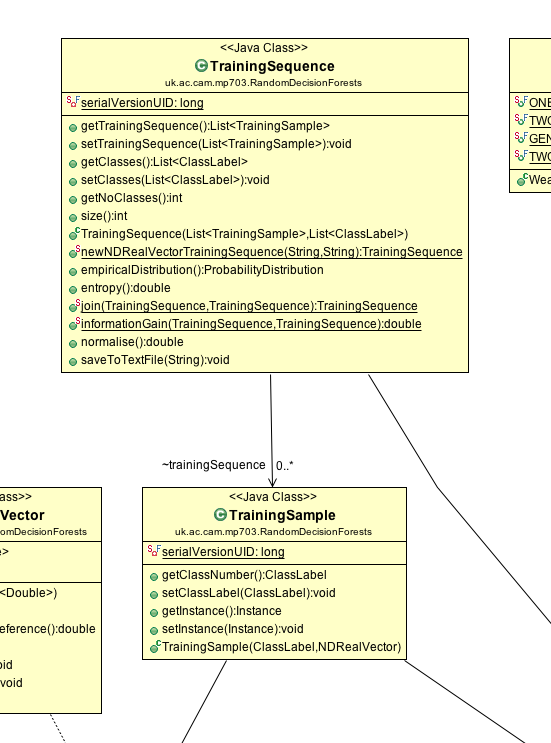
\includegraphics[scale=0.5]{TrainingSequence_Forest_UML}
                    \caption[A closer view of \texttt{TrainingSequence} and \texttt{TrainingSample}]{A closer view of \texttt{TrainingSequence} and \texttt{TrainingSample} in Figure \ref{fig:forest_uml}.}
                    \label{fig:training_seq_uml}
                \end{figure}

                \begin{table}[H]
                    \begin{tabularx}{\textwidth}{p{4.5cm}|X}
                        \textbf{Function Name} & \textbf{Function Description} \\
                        \hline

                        {\tt newNDRealVector\-TrainingSequence} & 
                            \texttt{newNDRealVectorTrainingSequence} is a \texttt{static} function taking two file names:
                            one specifying 
                            a ``class colour map'' file and one specifying a training sequence. Both these files should 
                            be of the format described in appendix \ref{app:file_formats}. This function parses the 
                            files and returns a \texttt{TrainingSequence} instance generated from it, with instances 
                            of the type \texttt{NDRealVector}. \\ 
                        \hline

                        \texttt{empericalDistribution} & 
                            Returns a \texttt{ProbabilityDistribution} that represents the empirical distribution of the 
                            training sequence, as defined in equation \ref{eq:empirical_distribution}. \\
                        \hline

                        \texttt{entropy} & 
                            This returns the entropy of the empirical distribution. It is essentially just a shorthand 
                            for calling \texttt{empiricalDistribution().entropy()}. \\
                        \hline

                        \texttt{join} & 
                            A \texttt{static} function that takes two \texttt{TrainingSequence}s, and joins them 
                            together. This simply appends the lists of \texttt{TrainingSample}s from two 
                            \texttt{TrainingSequence}s into a new \texttt{TrainingSequence} instance. \\
                        \hline

                        \texttt{informationGain} & 
                            A \texttt{static} function that takes two \texttt{TrainingSequence}s \texttt{ts1} and 
                            \texttt{ts2}. The function returns the information gain for splitting the training 
                            sequence \texttt{join(ts1,ts2)} into the training sequences \texttt{ts1} and \texttt{ts2} 
                            according to equation \ref{eq:information_gain}. \\
                        \hline

                        \texttt{normalise} & 
                            This parses all of the \texttt{Instance}s in the training sequence and computes an average 
                            ``normalisation reference'' (see \texttt{getNormalisationReference} in table 
                            \ref{tab:NDRealVector}). It then returns a new training 
                            sequence where every sample has been normalised to this average value. \\
                        \hline

                        \texttt{saveToTextFile} & 
                            This \texttt{static} function writes out a training sequence file with the data from the 
                            given \texttt{TrainingSequence} instance, in accordance with the file format specified in 
                            appendix \ref{app:file_formats}. \\
                        \hline

                        \texttt{bag} &
                            This performs bagging on a training sequence, and returns a bagged training sequence. The 
                            concept of \textit{bagging} is discussed in section \ref{sec:training}.

                    \end{tabularx}
                    \caption{Important methods implemented in the \texttt{TrainingSequence} class.}
                    \label{tab:TrainingSequence}
                \end{table}





            \subsubsection{Split Parameters} \label{sec:split_params}
                We define an abstract class \texttt{SplitParameters}, which is used as a common superclass for any 
                implementation of a split parameter, as defined in section \ref{sec:intro_decision_trees}. We 
                make this an abstract class so that it can implement \texttt{Serializable}, forcing
                any implementing classes to also implement this \texttt{Serializable}. Which is 
                necessary to be able to save decision forests to a file in section \ref{sec:DecisionForest}. 
                We also mention that each split parameter needs to be 
                able to specify what weak learner it is for, because we only save the split parameters in 
                decision trees and we need some way to determine which \texttt{WeakLearner} subclass to use from a 
                \texttt{SplitParameter} instance. 

                We also consider a concrete implementation of \texttt{SplitParameters}, in particular
                \texttt{OneDimensionalLinearSplitParameters} which specifies a ``dimension'' and a threshold as needed 
                for the \texttt{OneDimensionalLinearWeakLearner} in section \ref{sec:weak_learner}. 

                The \texttt{SplitParameter} classes are simple and only include getters, setters and constructors. 

                \begin{figure}[H]
                    \centering
                    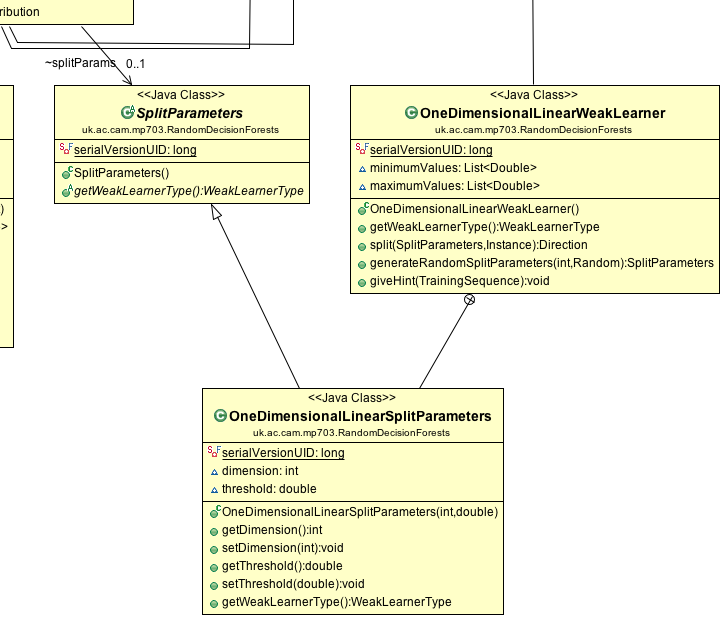
\includegraphics[scale=0.5]{SplitParam_Forest_UML}
                    \caption[A closer view of \texttt{SplitParamter}]{A closer view of \texttt{SplitParamter} and \texttt{OneDimensionalLinearSplitParameter} in figure \ref{fig:forest_uml}.}
                    \label{fig:split_param_uml}
                \end{figure}




            \subsubsection{Weak Learners} \label{sec:weak_learner}
                \texttt{WeakLearner} is implemented as an abstract class, because it provides a partial 
                implementation. Any common code between subclasses can be put directly into the \texttt{WeakLearner} 
                abstract class, such as helper functions for generation of randomised parameters. The function of each 
                abstract method is explained in table \ref{tab:OneDimensionalLinearWeakLearner}. The function 
                \texttt{uniformRandomDoubleInRange} is a simple convenience method that is used to generate a value 
                uniformly in some range \texttt{[lowerBound,highBound]}, 
                and uses Java's implementation of generating a uniform random variable in the range \texttt{[0,1]}. To 
                identify the type of each weak learner with some tag we define an \texttt{enum} type 
                \texttt{WeakLearnerType}, seen in Figure \ref{fig:weak_learner_type_uml}. 

                \begin{figure}[H]
                    \centering
                    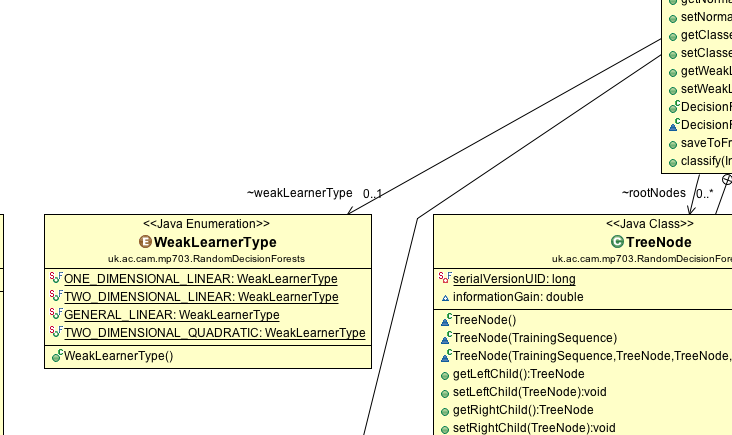
\includegraphics[scale=0.5]{WeakLearnerType_Forest_UML}
                    \caption{A closer view of the \texttt{WeakLearnerType} enum in Figure \ref{fig:forest_uml}.}
                    \label{fig:weak_learner_type_uml}
                \end{figure}

                We also consider a concrete implementation \texttt{OneDimensionalLinearWeakLearner} of the \texttt{WeakLearner}
                class. This is the most simple weak learner function that we could use and has the simplest parameters, 
                when we are considering \texttt{NDRealVector} instances. We note that subclasses of \texttt{WeakLearner}s are
                specific to particular subclasses of \texttt{Instance}. 
                The \texttt{OneDimensionalLinearWeakLearner} picks one value in the feature vector/instance, compares 
                it to some threshold and then makes a decision based on this. For example, consider an 
                instance $\vc{v} \in \bb{R}^n$. In this case our split parameters are $\vc{\theta} = (i,\tau) \in 
                \bb{Z}_n \times \bb{R}$, and the split function/weak learner is

                \begin{align}
                  f(\vc{v}; \vc{\theta}) = f(\vc{v}; (i,\tau)) = \begin{cases}
                    1 & \text{ if } v_i \geq \tau \\
                    0 & \text{ otherwise.}
                  \end{cases}
                  \label{eq:split_equation}
                \end{align}

                \begin{figure}[H]
                    \centering
                    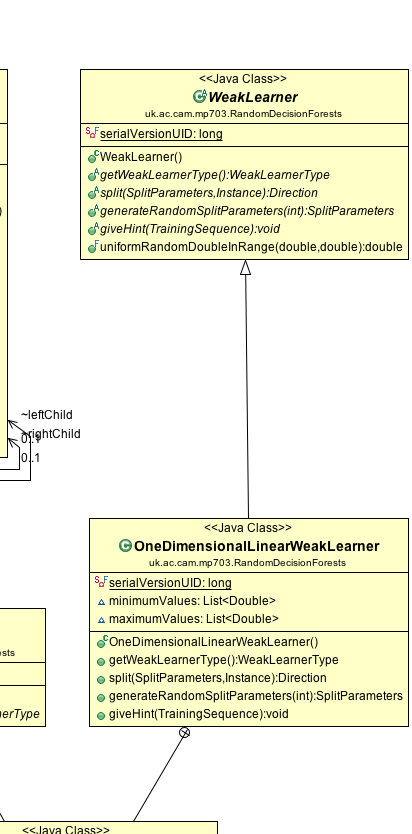
\includegraphics[scale=0.6]{WeakLearner_Forest_UML}
                    \caption[A closer view of \texttt{WeakLearner} and \texttt{DimensionalLinearWeakLearner}]{A closer view of \texttt{WeakLearner} and 
                    \texttt{DimensionalLinearWeakLearner} in Figure \ref{fig:forest_uml}.}
                    \label{fig:weak_learner_uml}
                \end{figure}

                These split parameters for the \texttt{OneDimensionalLinearWeakLearner} class are represented by the 
                \texttt{OneDimensionalLinearSplitParameters} class as described in section \ref{sec:split_params}. This 
                is an example that each subclass of \texttt{WeakLearner} should have a corresponding subclass of 
                \texttt{SplitParameters} which it uses to represent its split parameters. We note that 
                \texttt{OneDimensionalLinearSplitParameters} is implemented as a nested class within 
                \texttt{OneDimensionalLinearWeakLearner}, to make this relationship obvious.


                The \texttt{split} function is of particular interest in table \ref{tab:OneDimensionalLinearWeakLearner} as 
                it implements equation \ref{eq:split_equation}. 

                \begin{table}[H]
                    \begin{tabularx}{\textwidth}{l|X}
                        \textbf{Function Name} & \textbf{Function Description} \\
                        \hline

                        \texttt{getWeakLearnerType} & 
                            A function that is used to identify what type of weak learner an instance is. This is 
                            useful when a subclass is cast to \texttt{WeakLearner} and we want to cast it back to 
                            the subclass without causing an exception. \\ 
                        \hline

                        \texttt{split} & 
                            This function takes a split parameter and an instance, it is the concrete implementation 
                            of the split function. It returns an enum of type \texttt{Direction}, which specifies if 
                            we should traverse to the left or right child of a decision tree node. \\ 
                        \hline

                        \texttt{giveHint} & 
                            In this function we are passed the training sequence prior to training a decision tree. 
                            It is used as a chance to look at the data to give a hint to what split parameters we 
                            might want to generate, or more specifically not generate. \\ 
                        \hline

                        \texttt{generateRandomSplitParameters} & 
                            This function provides a routine for generating a random split parameter to be tried in the 
                            split function during training a decision tree. \\ 

                    \end{tabularx}
                    \caption[The methods of \texttt{OneDimesnionalLinearWeakLearner}.]{Important methods implemented in the \texttt{OneDimensionalLinearWeakLearner} class.}
                    \label{tab:OneDimensionalLinearWeakLearner}
                \end{table}

                The \texttt{OneDimensionalLinearWeakLearner} makes use of the \texttt{giveHint} function by iterating through 
                all \texttt{NDRealVector} instances in the training sequence and recording a minimum and maximum value 
                for each dimension in the lists \texttt{minimumValues} and \texttt{maximumValues}. This  
                allows us to avoid picking particularly bad \texttt{OneDimensionalLinearSplitParameters}. 
                For any of the features/dimensions in the \texttt{NDRealVector} 
                that are chosen, if we pick a threshold value outside the range between the minimum and maximum we know that 
                the split function will split the training sequence with zero information gain. Using the notation from 
                equations \ref{eq:left_split} and \ref{eq:right_split} it means that one of $L(\vc{s},\vc{\theta})$ or 
                $R(\vc{s},\vc{\theta})$ will be empty, leading to an information gain of zero ($I(\vc{s},\vc{\theta}) = 0$ 
                in equation \ref{eq:information_gain}).




            \subsubsection{Decision Tree Node}
                Finally we move onto defining our decision tree, implement the \texttt{TreeNode} class nested in 
                \texttt{DecisionForest} to show that their behaviour is tightly coupled. Each node has a reference 
                to a left and right child node, which are set to \texttt{null} in a leaf node. Every node caches a 
                probability distribution, even if it is a decision node, and the 
                probability distribution that is cached is the empirical distribution of the training sequence that is 
                passed to it. Each decision node has a reference to a \texttt{SplitParameters} instance, which it 
                uses with a weak learner to make decisions for tree traversal as in section 
                \ref{sec:intro_decision_trees}. We then cache the information gain, computing it according to the 
                equation \ref{eq:information_gain} during the training algorithm.

                \begin{figure}[H]
                    \centering
                    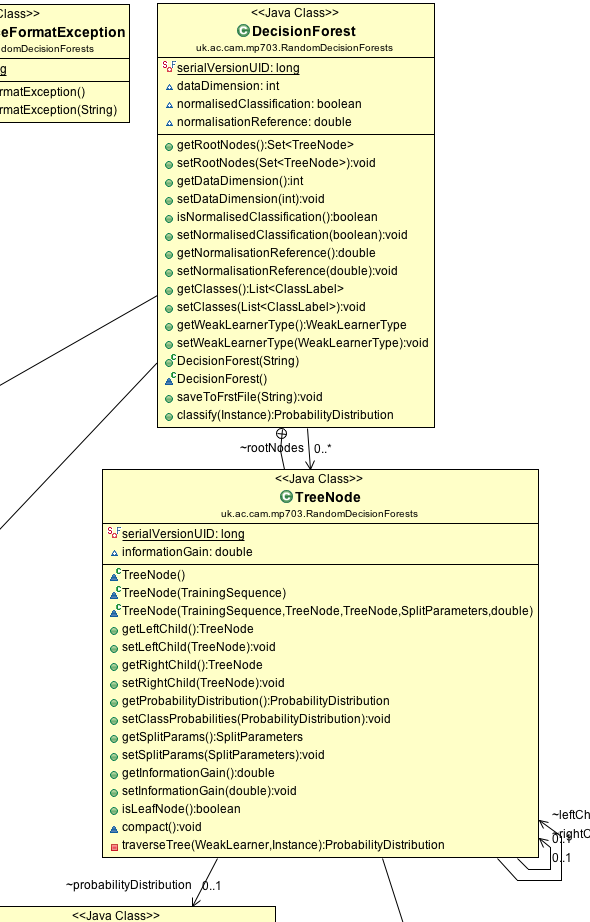
\includegraphics[scale=0.5]{Tree_Forest_UML}
                    \caption{A closer view of \texttt{TreeNode} and \texttt{DecisionForest} in Figure \ref{fig:forest_uml}.}
                    \label{fig:weak_learner_uml}
                \end{figure}

                The function \texttt{compact} is seen in listing \ref{lst:TreeNode}. This is an optimisation 
                used to eliminate unnecessary nodes from the tree after its construction. If we are at 
                some decision node and it has two children which are leaf nodes with identical distributions, then we 
                can replace this decision node by a single leaf node with the same distribution. The implementation 
                performs \texttt{compact} recursively on the left and right children of a decision node first, 
                and \texttt{compact} does nothing in the base case (a leaf node), after we try to compact at the 
                given node. Essentially, compaction is performed from the bottom of the tree upwards.

                We also note that the \texttt{TreeNode} class implements the \texttt{Serializable} interface, 
                which is again necessary to be able to use \texttt{ObjectOutputStream} in section 
                \ref{sec:DecisionForest}, when saving forests to a file.

                \begin{lstlisting}[float=tp,caption={[The \texttt{TreeNode} declaration.] The \texttt{TreeNode} declaration, found as a static class within the 
                \texttt{DecisionForest} class.},label={lst:TreeNode}]
void compact() throws MalformedForestException {
  if (this.isLeafNode()) {
    return;
  }
  
  this.leftChild.compact();
  this.rightChild.compact();

  if (!this.isLeafNode() && 
      leftChild.isLeafNode() &&
      rightChild.isLeafNode() &&
      probabilityDistribution.equals(leftChild.probabilityDistribution) &&
      probabilityDistribution.equals(rightChild.probabilityDistribution)) {
    
    // Make this node a leaf node
    leftChild = null;
    rightChild = null;
  }
}
                \end{lstlisting}

                \begin{table}[H]
                    \begin{tabularx}{\textwidth}{l|X}
                        \textbf{Function Name} & \textbf{Function Description} \\
                        \hline

                        \texttt{isLeafNode} & 
                            Checks if the \texttt{leftChild} and \texttt{rightChild} have a value of \texttt{null}. If 
                            they do then the node is a leaf and this functions returns a true value. If only one of the 
                            nodes has a value of \texttt{null} then the tree is invalid and an exception is raised. 
                            Otherwise it returns a false value. \\ 
                        \hline

                        \texttt{compact} & 
                            As described above, this compacts the tree to an equivalent tree, replacing any unnecessary 
                            decision nodes with a leaf node. \\ 
                        \hline

                        \texttt{traverseTree} &
                            A method that given an instance of a \texttt{WeakLearner} and an \texttt{Instance} will 
                            traverse the tree and return a probability distribution for that instance. As described in 
                            section \ref{sec:intro_decision_trees} and visualised in figure 
                            \ref{fig:decision_tree_classify}. The algorithm this method implements is covered in more 
                            detail in section \ref{sec:classification}.

                    \end{tabularx}
                    \caption{Important methods implemented in the \texttt{TreeNode} class.}
                    \label{tab:TreeNode}
                \end{table}




            \subsubsection{Decision Forest} \label{sec:DecisionForest}
                The \texttt{DecisionForest} class is basically a set of \texttt{TreeNode}s, which also includes 
                additional metadata, that which can be seen in Figure \ref{fig:weak_learner_uml}. 
                We have made sure that \texttt{TreeNode}, \texttt{WeakLearner}, \texttt{WeakLearnerType}, 
                \texttt{SplitParameters} and \texttt{ClassLabel} (which are all composite in the forest data structure) 
                implement the interface \texttt{Serializable} so that a concise ``save to file'' method can be 
                implemented. We use an instance of \texttt{ObjectOutputStream} in the \texttt{Java.Io} package 
                to write the object to a binary file in a single line ``\texttt{out.writeObject(this);}''.

                \texttt{dataDimension} keeps track of the dimension of data this forest classifies, while the 
                \texttt{weakLearnerType} specifies what weak learner our forest is related to, and implicitly the type 
                of data that it classifies. The \texttt{DecisionForest} keeps a reference to all the possible classification labels in 
                the variable \texttt{classes} of type \texttt{List<ClassLabel>}. \texttt{DecisionForest} uses 
                \texttt{normalisedClassification} and \texttt{normalisationReference} to 
                perform normalisation during classification, if we specified that normalised values should be used during 
                training.

                \begin{table}[H]
                    \begin{tabularx}{\textwidth}{l|X}
                        \textbf{Function Name} & \textbf{Function Description} \\
                        \hline

                        \texttt{DecisionForest} & 
                            We have a \texttt{default} access 
                            default constructor, which is used to construct forests in the training algorithm. The 
                            other allows the forest to be loaded from a file using an \texttt{ObjectInputStream} from 
                            the \texttt{Java.Io} package. \\ 
                        \hline

                        \texttt{saveToFrstFile} & 
                            This function saves a forest to a persistent ``.frst'' file. \\ 
                        \hline

                        \texttt{classify} & 
                            This takes an \texttt{Instance} and returns a probability distribution for it, according 
                            to the forest. The algorithm implementation is discussed in more detail in section 
                            \ref{sec:classification}. \\ 

                    \end{tabularx}
                    \caption{Important methods implemented in the \texttt{DecisionForest} class.}
                    \label{tab:DecisionForest}
                \end{table}






      \subsection{Training} \label{sec:training}
          The concept of training was discussed in section \ref{sec:supervised_learning} and an overview of 
          how we can train decision trees and decision forests in section \ref{sec:rand_forest}. This section provides 
          some simple psuedocode to generate trees given a training sequence, then extends it for training a decision forest. We 
          then discuss some design choices for an implementation of the algorithm, problems that may be encountered and 
          some possible solutions to those problems.

          \begin{lstlisting}[float=tp,caption={Psuedocode to train a decision tree.}, label={lst:generateTree}]
TreeNode generateTree(trainingSequence, depth, randomnessParameter) {
  // Base (terminating) case
  if (depth <= 0) {
    return new TreeNode(trainingSequence);
  }

  // Remember the best split
  bestInfoGain = 0.0;
  bestLeftSplit = null;
  bestRightSplit = null;

  // Try [randomnessParameter] number of times
  for (int i = 0; i < randomnessParameter; i++) {
    
    // Split
    splitParameter = generateRandomSplitParameter();
    for (sample in trainingSequence) {
      // 'split' is our split function
      if (split(sample, splitPerameter) == 0) {
        leftSplit.add(sample);
      } else {
        rightSplit.add(sample);
      }
    }

    // Update best if necessary
    infoGain = informationGain(leftSplit, rightSplit)
    if (infoGain > bestInfoGain) {
      bestInfoGain = infoGain;
      bestLeftSplit = leftSplit;
      bestRightSplit = rightSplit;
    }
  }

  // Recurse
  leftChild = generateTree(bestLeftSplit, depth-1, randomnessParameter);
  rightChild =  generateTree(bestRightSplit, depth-1, randomnessParameter);

  // Return the tree
  return new TreeNode(leftChild, rightChild)
}
          \end{lstlisting}

          \clearpage
          The full code listing for training a decision tree is given in listing \ref{lst:actualGenerateTree}. The value 
          \texttt{randomnessParameter} is the value $\rho$ from section \ref{sec:moving_swiftly_onto_forests}. The algorithm 
          abstracts away from using a single weak learner and the \texttt{WeakLearner} class specifies functions 
          synonymous to the \texttt{generateRandomSplitParameter} and \texttt{split} used in listing \ref{lst:generateTree}.
          This allows the algorithm for training to be written in a generic way and allowing for high code re-usability. 

          There are a number of things to consider when implementing this algorithm if we wish to return useful and 
          efficient trees. Firstly, deep trees (specified by a high depth) may be necessary to provide correct 
          classifications in large multi-class problems, however as we get deeper into the tree, decision nodes could 
          be adding little information. I.e. consider when we have a empirical distribution at depth 
          3 which is almost identical to the distribution found 
          at depth 20, in this case the decisions made at depths 3 to 20 have made very little difference to the output 
          and effectively waste computation time. To ameliorate the problem we can provide a threshold value for the 
          information gain, which if not surpassed at some node causes the training to terminate. This is included in 
          the implementation seen in listing \ref{lst:actualGenerateTree} with the parameter \texttt{informationGainCutoff}. 

          Secondly we consider the generation of split parameters. Sometimes with prior information, or even analysis 
          of the training sequence, a more informed choice of split parameter can be made. We talk about this at the 
          end of section \ref{sec:weak_learner}, when we discuss optimising \texttt{OneDimensionalWeakLearner} parameter 
          selection. The optimisation discussed is included in the \texttt{OneDimensionalWeakLearner} implementation.

          In listing \ref{lst:generateTree} we see that the tree is trained depth first, 
          alternatively a breadth first approach can be imagined, as in Figure \ref{fig:breadth_first}. In breadth first 
          training we train all nodes at some depth at the 
          same time and optimise over the collective information gain. In the implementation in listing
          \ref{lst:actualGenerateTree} we decide to implement a depth first algorithm, as it is easier to parallelise 
          (and distribute if wanted), because each of the child nodes are trained independently.

          \begin{figure}
              \centering
              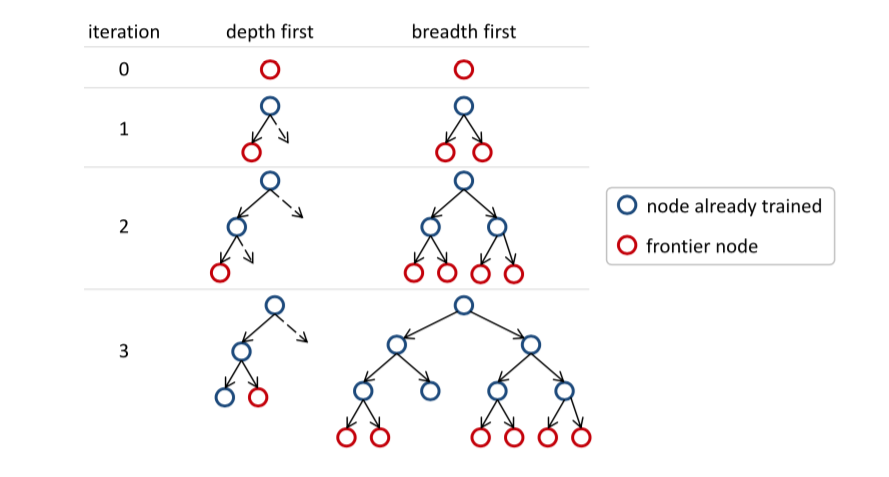
\includegraphics[scale=0.3]{breadthfirst_vs_depthfirst}
              \caption[Visualisation of breadth first vs depth first.]{Visualisation of breadth first vs depth first. Optimisation of information gain takes place over 
              all of the nodes in the frontier. Recreated from Criminisi et al \cite{criminisi2013decision}.}
              \label{fig:breadth_first}
          \end{figure}

          The algorithm for training a decision forest extends easily from training a decision tree and psuedocode is 
          given in listing \ref{lst:train}.

          \begin{lstlisting}[float=tp,caption={Psuedocode to train a decision forest.},label={lst:train}]
DecisionForest train(trainingSequence, noTrees, 
  depth, randomnessParameter) {

  rootNodes = [];
  for (int i = 0; i < noTrees; i++) {
    subSequence = trainingSequence.bag();
    treeNode = 
      generateTree(subSequence, depth, randomnessParameter);
    rootNodes.add(treeNode);
  }

  return new DecisionForest(rootNodes);
}
          \end{lstlisting}

          In listing \ref{lst:train} the training sequence is `bagged' for each tree, which yields a subsequence of the 
          training sequence, used to train that tree. The term \textit{bagging} refers to taking a subsequence 
          of the training sequence and using that for training. Generally it is used as a way to introduce randomness and 
          combat over-fitting. One problem which is commonly encountered and leads to over-fitting is when 
          on class of data is abundantly present in the training sequence, and another class of data isn't \cite{criminisi2013decision}. 
          In this case the abundant data will have a large influence 
          on the information gain from equation \ref{eq:information_gain}. We 
          can deal with this problem either by weighting the influence of each class inversely by the number of samples it has in equation 
          \ref{eq:information_gain}, or by bagging in such a way that each tree is trained on a sequence with equal 
          numbers of samples from each class. In our implementation in listing \ref{lst:actualTrainForest} we take the 
          later approach. 

          Another trick that can be used to reduce over-fitting is to increase the randomness of our choice of 
          split parameters. Which is implemented by a low value for $\rho$ or \texttt{randomnessParameter}. One option 
          is to start with a low value of $\rho$ at high depths in the tree and increase it at lower depths. This is 
          not included in our implementation.

          Finally there is some obvious parallelism to exploit again, where each tree can be independently trained 
          in it's own thread. This is a feature of the actual implementation and can be seen in listing 
          \ref{lst:actualTrainForest}.






      \subsection{Classification} \label{sec:classification}
          As discussed in section \ref{sec:moving_swiftly_onto_forests} we classify by walking along each tree and 
          averaging over the different distributions. Psuedocode for traversing the tree is given in listing 
          \ref{lst:traverseTree} and psuedocode for classification is given in listing \ref{lst:classify}.

          \begin{lstlisting}[float=tp,caption={Psuedocode for traversing a decision tree.}, label={lst:traverseTree}]
ProbabilityDistribution traverseTree(instance) {
  currentNode = this;
  while (!isLeaf(currentNode)) {
    direction = split(currentNode.splitParams, instance);
    if (direction == LEFT) {
      currentNode = currentNode.leftChild;
    } else {
      currentNode = currentNode.rightChild;
    }
  }

  // When we get here we are a leaf node
  return currentNode.probabilityDistribution;
}
          \end{lstlisting}

          \begin{lstlisting}[float=tp,caption={Psuedocode for classification using a decision tree.}, label={lst:classify}]
public ProbabilityDistribution classify(instance) {
  for (node in rootNodes) {
    if (accumulatingDistr == null) {
      accumulatingDistr = node.traverseTree(instance);
      treesTraversed++;
    } else {
      leafDistr = node.traversTree(instance);
      accumulatingDistr.addRunningTotal(leafDistr, ++treesTraversed);
    }
  }
  return accumulatingDistr;
}
          \end{lstlisting}

          Similar to the learning algorithm, parallelism can be exploited from traversing each tree in a separate 
          thread, and again is in the implementation found in listing \ref{lst:classify}. We make use of the 
          \texttt{addRunningTotal} function that we defined in section \ref{sec:prob_dist} so that we sum in a 
          numerically stable fashion. There is not much more that can be said about the classification algorithm for 
          random forests, its simplicity is one of its major advantages.






    \section{Neural Networks} \label{sec:nn_training} \label{sec:pixel_label}
        For our neural network solution we use a standalone Java neural network library, Encog. Following Encog's quickstart 
        guide\footnote{https://s3.amazonaws.com/heatonresearch-books/free/encog-3\_3-quickstart.pdf} it is very easy to 
        set up a simple neural network. Then using Encog's user 
        guide\footnote{https://s3.amazonaws.com/heatonresearch-books/free/Encog3Java-User.pdf} gives us a better 
        understanding of Encog's architecture and how it can be manipulated into what we want.         

        \begin{figure}
            \centering
            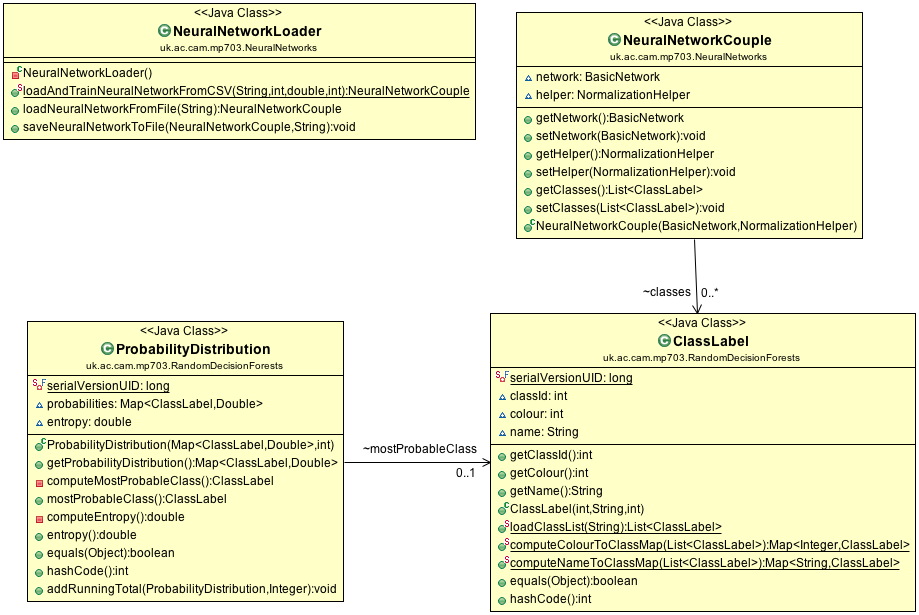
\includegraphics[scale=0.4]{NeuralNet_UML}
            \caption{The UML diagram for the Neural Net package.}
        \end{figure}

        Using the Encog api we build a 4 layer network. We set the activation function to sigmoid functions for the 
        two hidden layers and a softmax activation function for the output layer. Recall the syntax we defined in section 
        \ref{sec:neuralnetworkdef}, if we have a softmax activation function at layer $L$ then we set 

        \begin{align}
            a_k^L = \frac{e^{-z_k^L}}{\sum_i e^{-z_i^L}}
            \label{eq:softmax_defn}
        \end{align}

        where

        \begin{align}
            z_k^L = \sum\limits_j w_{jk}^L a_j^{L-1} + b_k^L.
            \label{eq:activationinput}
        \end{align}

        Despite equation \ref{eq:activationinput} looking quite scary, it is just the weighted sum of activations from 
        layer $L-1$ at node $k$ in layer $L$. From equation \ref{eq:softmax_defn} we see that the activations at layer 
        $L$ sum to one, which makes it useful on an output layer so that a probability distribution can be output. 

        \begin{figure}
            \centering
            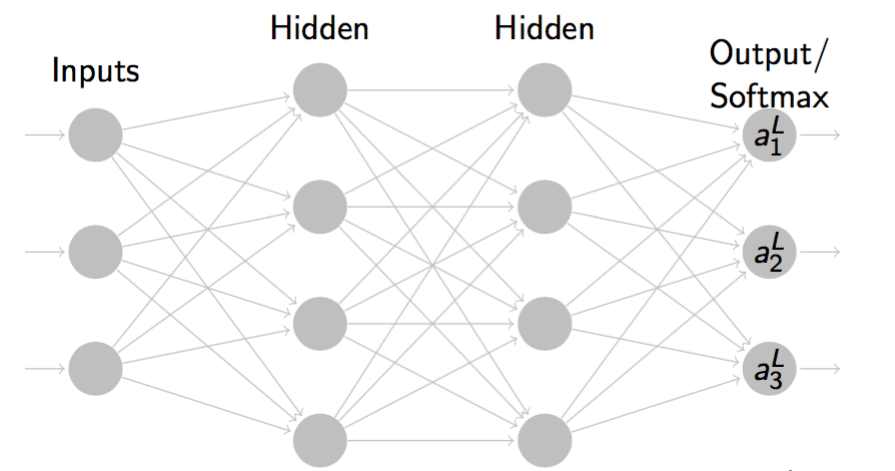
\includegraphics{softmax_neuralnetworks}
            \caption{The architecture of our neural network for classification.}
        \end{figure}

        This reduces the neural network to the situation found in equation \ref{eq:weird_hyp}, allowing us to provide 
        a classification. However we need to modify our training sequence slightly, instead of specifying a class as the 
        example output, we must replace it with a probability distribution. So for a training sample $(\vc{x}_i, c_i)$ we
        we give the network the training sample $(\vc{x}_i, p_c)$ where 

        \begin{align}
            p_c(c') = \begin{cases} 
                1 & \text{ if } c' = c \\
                0 & \text{ otherwise.}
            \end{cases}
        \end{align}

        \begin{lstlisting}[caption={[Simple construction of our neural network in Encog.]Simple construction of our neural network in Encog, where \texttt{dataDimension} is the number of spectral bins we have in spectra to classify and \texttt{noClasses} is the number of classes.},label={lst:network_def}]
BasicNetwork network = new BasicNetwork();
network.addLayer(new BasicLayer(null, true, dataDimension));
network.addLayer(new BasicLayer(new ActivationSigmoid(), true, dataDimension));
network.addLayer(new BasicLayer(new ActivationSigmoid(), true, dataDimension));
network.addLayer(new BasicLayer(new ActivationSoftmax(), true, dataDimension));
network.getStructure().finalizeStructure();
network.reset(); // randomise weight values
        \end{lstlisting}

        Training and classification using the neural network are as simple to implement as listing \ref{lst:network_def}, however are omitted for brevity.







    \section{Pixel Labelling}
        In the Pixel Labelling module we are concerned with using either a decision forest or a neural network to 
        perform a pixel labelling. Both implementations output a probability distribution, which can be used to 
        generate a number of interesting images. This section begins with a brief discussion on how we perform the 
        pixel labelling and then we move onto different types of images that we can output.

        \begin{figure}
            \centering
            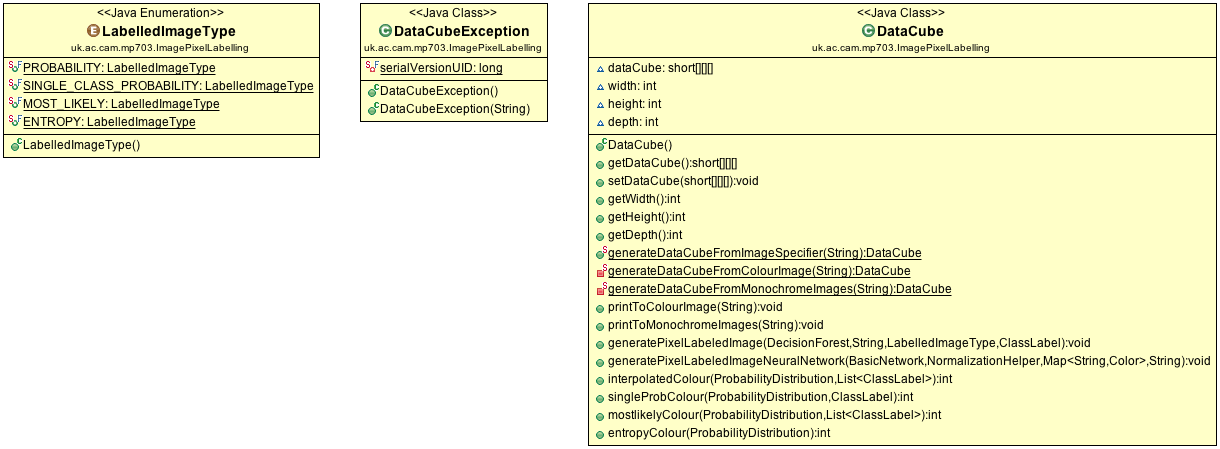
\includegraphics[scale=0.3]{PixelLabel_UML}
            \caption{The UML diagram for the pixel labelling module.}
        \end{figure}

        Supposed we have loaded in a spectral image $I$ using the \texttt{dataCube} class, then implementation of the 
        pixel labelling method \texttt{generatePixelLabeledImage} proceeds as follows:
        \begin{enumerate}
            \item 
                Create a blank image, with the same width and hight as $I$.
            \item 
                For each pixel $(x,y)$:

                \renewcommand{\labelenumii}{\theenumi.\arabic{enumii}.}
                \begin{enumerate}
                    \item 
                        Pass the spectrum $I(x,y,\cdot)$ to the appropriate machine learning implementation which provides 
                        and output probability distribution.
                    \item 
                        Pass the probability distribution to some function that will compute a colour value to set at $(x,y)$ in the pixel labelling.
                \end{enumerate}
                \renewcommand{\labelenumii}{(\alph{enumii})}

        \end{enumerate}

        In the implementation there is a number of ways that we can label each pixel based off the probability 
        distribution, which will now be defined. Let $p:\cl{C}\rightarrow [0,1]$ be some probability distribution at a 
        pixel $(x,y)$. Let $\alpha:\cl{C}\rightarrow \bb{N}_{255}^3$ be a function mapping from classes to the set of RGB 
        colours. We have the following options for producing a label:
        \begin{description}
            \item[Most Likely:]
                Pick the `most likely' label, then label the pixel with the colour $\alpha(c)$ determined by $c_{\text{max}} = \argmax_c p(c)$.
            \item[Weighted Average:]
                 Return a weighted average of class colours. This can be a nice way to look at the output for a small number of classes, however can be messy for larger number of classes. It returns the colour $(\sum_{c\in\cl{C}} p(c)\alpha(c))/|\cl{C}|$.
            \item[Entropy:]
                 Returns a (normalised between 0 and 255) grey scale value for the entropy. If entropy is high for $p$ then it tells us that we are uncertain about what class we should label the image. If we output both an entropy image and a most likely pixel labelling, the entropy image can be used as a measure of uncertainty in the classification given.
            \item[Probability in a class:]
                  We can specify a single class $c$, for which we return a grey scale value of $255 \cdot p(c)$ at the pixel. 
        \end{description}

        \clearpage
        \begin{figure}
            \begin{minipage}{0.49\textwidth}
                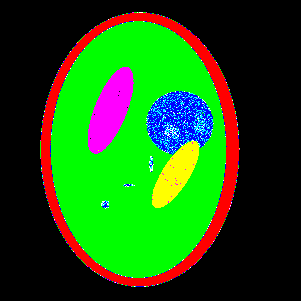
\includegraphics[scale=0.60]{example_mostlikely}
            \end{minipage}
            \hfill
            \begin{minipage}{0.49\textwidth}
                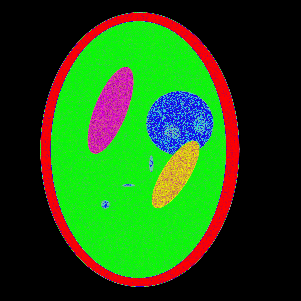
\includegraphics[scale=0.60]{example_probout}
            \end{minipage}
            \begin{minipage}{0.49\textwidth}
                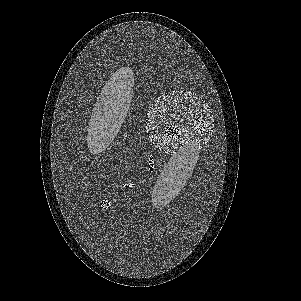
\includegraphics[scale=0.60]{example_entropy}
            \end{minipage}
            \hfill
            \begin{minipage}{0.49\textwidth}
                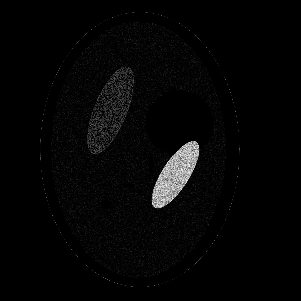
\includegraphics[scale=0.60]{example_singleprob}
            \end{minipage}
            \centering
            \begin{minipage}{0.49\textwidth}
                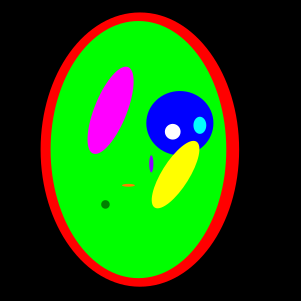
\includegraphics[scale=0.72]{example_groundtruth}
            \end{minipage}
        \caption[The four possible pixel labellings types we can output.]{Example (on an image corrupted by Poisson noise with no de-noising) of outputs of the four possible pixel labellings types we can output: most likely, weighted average, entropy and probability for a single class (with class colour yellow). The fifth image at the bottom left is the ground truth pixel labelling. The outputs for this image were determined from a decision forest with parameters: (noTrees,treeDepth,$\rho$) = (1000, 4, 1).}
        \end{figure}








    \section{Training Tools} \label{sec:training_tools}
        At this point we now have a system capable of producing pixel labellings. This section is concerned with 
        making the task of generating a training sequence feasible, as it is certainly not by hand. It would be 
        preferable to have some way of taking a ``ground truth'' pixel labelling and transforming it into a training 
        sequence. This is precisely what the training tools module does. 

        \begin{figure}[H]
            \centering
            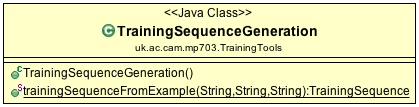
\includegraphics[scale=0.5]{TrainingTools_UML}
            \caption[The UML diagram for the training tools module.]{The UML diagram for the training tools module, consisting of a single class with a single static method.}
        \end{figure}

        \begin{figure}
            \centering
            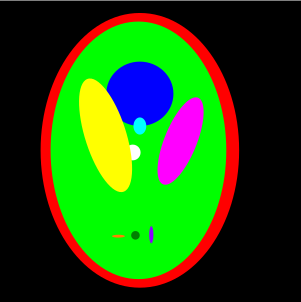
\includegraphics[scale=0.8]{example_pixel_label_shepp_logan} 
            \ \ \ 
            
\includegraphics[scale=0.33]{example_spectral_image_shepp_logan}
            \begin{framed}
                {\tt\raggedright
                    Skeleton, 0xFF0000,     \\
                    Tissue, 0x00FF00,       \\
                    LeftOrgan, 0xffff00,    \\  
                    CentreOrgan, 0x0000ff,  \\
                    RightOrgan, 0xff00ff,   \\
                    Artifact1, 0x00ffff,    \\
                    Artifact2, 0xffffff,    \\
                    Artifact3, 0xff7f00,    \\
                    Artifact4, 0x008100,    \\
                    Artifact5, 0x8c00ff,    \\
                    Background, 0x000000    \\
                } 
            \end{framed}
            \caption[An example input to the training tools module.]{An example input to the training tools module: a ground truth pixel labelling, a spectral image 
            and a class to colour mapping file (as defined in appendix \ref{app:file_formats}).}
        \end{figure}

        \begin{figure}
            \begin{framed}
                {\tt
                  ... \\
                  Artifact3, 140.0, 140.0, 141.0, 141.0, 140.0, 139.0, 145.0, 148.0, 148.0, 149.0, 148.0, 150.0, 147.0, 145.0, 143.0, 140.0, 140.0, 141.0, 141.0, 140.0, 140.0, 140.0, 141.0, 139.0, 140.0, 139.0, 140.0, 140.0, 139.0, 139.0; \\
                  Tissue, 91.0, 92.0, 90.0, 91.0, 91.0, 92.0, 95.0, 94.0, 100.0, 104.0, 105.0, 104.0, 100.0, 99.0, 96.0, 95.0, 94.0, 95.0, 91.0, 89.0, 89.0, 91.0, 90.0, 90.0, 91.0, 91.0, 92.0, 90.0, 91.0, 90.0; \\
                  ... 
                } 
            \end{framed}
            \caption[Example of part of the output file from the training tools module]{Example of part of the output file (2 training samples) from the training tools module. (The actual file is over 88000 lines long).}
        \end{figure}

        The function \texttt{trainingSequenceFromExample} performs the following sequence of actions:
        \begin{enumerate}
            \item 
                Load the list of classes into a \texttt{List<ClassLabel>} object and uses 
                \texttt{computeColourToClassMap} in \texttt{ClassLabel} to compute a map from colours to classes.
            \item 
                Load in the ground truth pixel labelling and the spectral image into the \texttt{DataCube} object from 
                section \ref{sec:pixel_label}.
            \item 
                For each pixel $(x,y)$:   
                \renewcommand{\labelenumii}{\theenumi.\arabic{enumii}.}
                \begin{enumerate} 
                    \item
                        Put the spectrum at $(x,y)$ into a \texttt{NDRealVector} instance.
                    \item 
                        Lookup the correct \texttt{ClassLabel} object from the map computed in step 1, using the colour 
                        in the ground truth image at $(x,y)$.
                    \item 
                        Pair the \texttt{ClassLabel} and \texttt{NDRealVector} together in a \texttt{TrainingSample} and 
                        put it into an accumulating training sequence.
                \end{enumerate}
                \renewcommand{\labelenumii}{(\alph{enumii})}
            \item 
                Return the accumulated training sequence.
        \end{enumerate}

        When using the training tools module through the \texttt{.jar} file, the interface adds an extra step to the end, 
        using the \texttt{saveToTextFile} function of the \texttt{TrainingSequence}, which saves and formats the 
        sequence to a text file. We can also use the \texttt{.jar} to pass the generated \texttt{TrainingSequence} 
        directly to the one of the training functions specified in sections \ref{sec:training} and \ref{sec:nn_training}.

        If an `invalid' colour is encountered in the example labelling we have two reasonable options, either raise an 
        exception or just ignore the spectrum for that pixel. In our implementation we decide to opt for the latter, as it 
        provides greater flexibility to use the system when input data isn't perfect, for example in figure 
        \ref{fig:non_perfect_labelling}.

        \begin{figure}
            \centering
            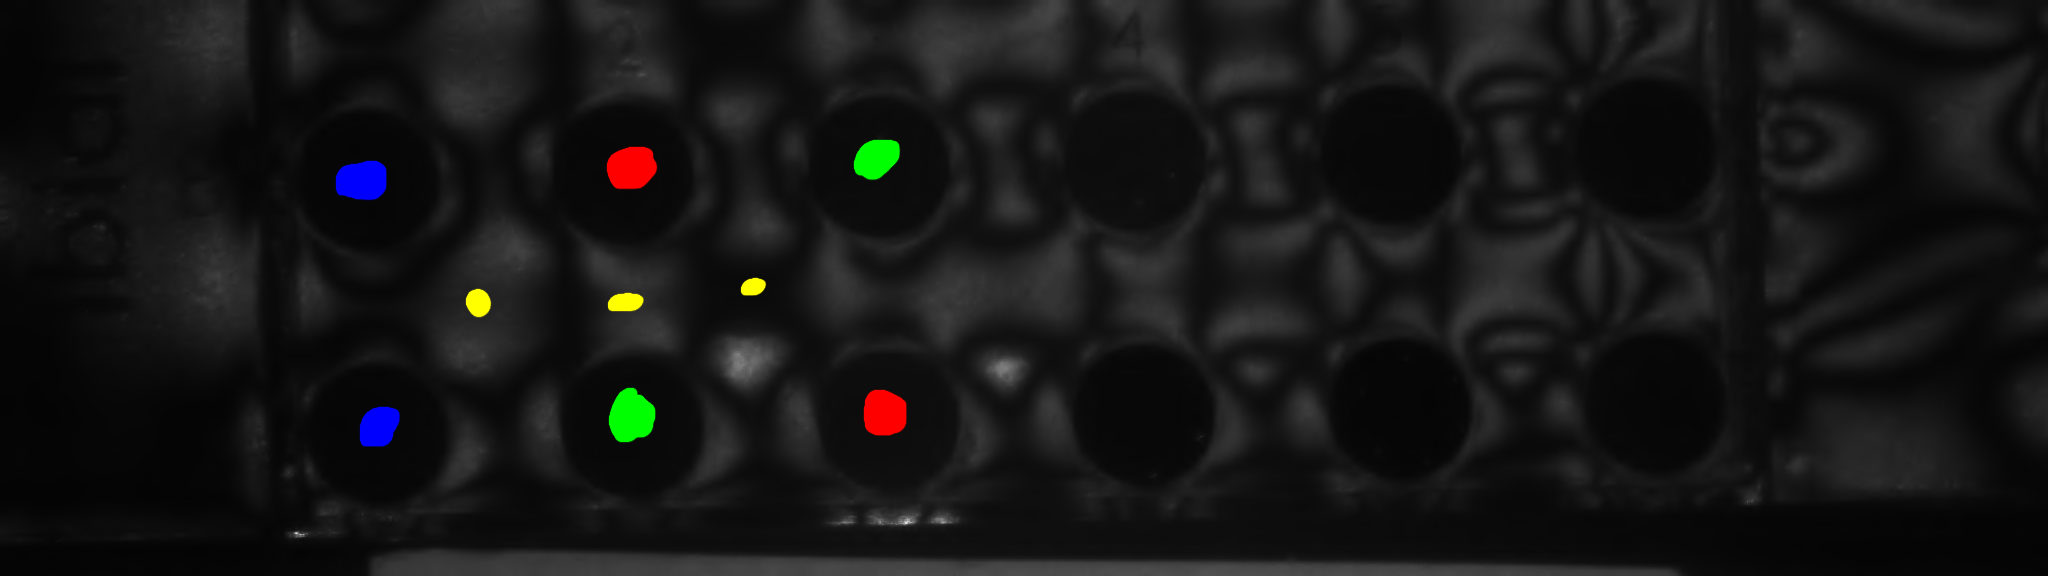
\includegraphics[scale=0.2]{example_pixel_label_siri}
            \caption[An example of a noisy `ground truth' pixel labelling.]{An example of a `ground truth' pixel labelling we might want to provide when data is noisy or irrelevant, when we wish to ignore large regions of the image.} 
            \label{fig:non_perfect_labelling}
        \end{figure}






    \section{De-noising} \label{sec:de-noising}
        Many of the images that we will need to deal with will exhibit noise. In this section we justify our need to
        deal with noise in our system, and then discuss our implementation of the noise package. Possible models for 
        noise in imaging are discussed in appendix \ref{app:img_noise}. 

        In image processing systems for a medical purpose must be accounted for somehow, many methods 
        of medical imaging utilise ionising radiation that would be considered harmful given extended exposure times 
        \cite{picano2004sustainability}. As a consequence there is an inherent trade off between exposure time (for 
        greater image clarity) and risk of causing damage \cite{sprawls1987physical}. Since we may potentially 
        require use shorter exposure times it is often found that quantum noise (defined in appendix \ref{app:img_noise}) 
        is more appropriate than a Gaussian noise due to. There are many cases 
        such as ultrasound where we may want to consider more sophisticated noise models \cite{coupe2009nonlocal}, 
        but for the purpose of this dissertation we will restrict ourselves to the noise models defined in appendix \ref{app:img_noise}. 

        \begin{figure}
            \centering
            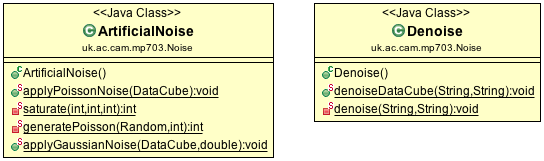
\includegraphics[scale=0.5]{Noise_UML}
            \caption{The UML diagram for the Noise package.}
        \end{figure}

        Lots of algorithms that perform image de-noising, such as Total Variance Majorisation-Minimisation \cite{figueiredo2006total} 
        require large amounts of numerical computation. In the preparation phase it became quickly apparent that image 
        de-noising is a complicated task, and implementing it well could be a project in it's own right. In the interest 
        of both time and quality of the end product the decision was made to use a library implementation. The function 
        \texttt{Denoise.denoise} is a wrapper for the \texttt{BoofCV} library implementation of de-noising 
        \cite{BoofCV2012}.



    \section{Application on example data sets}
        \begin{itemize}
            \item We've build a system, but we need to actually apply it to some problems!
        \end{itemize} 

        \subsection{Siri's data}
            \begin{itemize}
                \item TODO: Come up with a better title for this subsection
                \item Explanation of how produced training data
                \item Example pixel labellings
            \end{itemize}








%%%%%%%%%%%%%%%%%%%%%%%%%%%%%%%%%%%%%%%%%%%%%%%%%%%%%%%%%%%%%%%%%%%%%%%%%%%%%%%%%%%%%%%%%%%%%%%%%%%%%%%%%%%%%%%%%%%%%%%%
% the evaluation

\cleardoublepage
\chapter{Evaluation}
    In this section we will look at the performance of the different components of the system based on a number of 
    metrics. 

    \section{Performance measures for classifiers}
        \begin{itemize}
            \item Briefly say about the different measures as described at the end of AI II.
            \item Justify what might be the most informative here.
        \end{itemize}

    \section{Evaluation of the Random Forests library}
        \begin{itemize}
            \item Define a standard training set, this can actually be independent of pixel labelling and similar to the Chriminsi forests paper.
        \end{itemize}

        \subsection{Training time}
        \subsection{Classification time}
        \subsection{The effect of the number of trees}
        \subsection{The effect of the depth of trees}
        \subsection{The effect of the randomness of trees}
        \subsection{The effect of normalisation} \label{sec:effect_of_normalisation}


    \section{The effect of the de-noising component}
        \begin{itemize}
            \item Use a couple images with added noise
            \item Compare the SNR for the method with respect to different noise models (does it handle any other types of noise?)
            \item Plot SNR as a function of the parameter lambda in the TVMM method
            \item Plot SNR as a function of noise power (for different types of noise)
        \end{itemize}


    % \section{Performance speed ups in OpenCL}=
    % *TODO* - compare to classification time with OpenCL in encog turned on, also compare to non openCL time.
    % Compare the classification times with openCL on/off in encog.


    % \section{Evaluation of the analysis module}
    %     \begin{itemize}
    %         \item Made for Siri's data set
    %         \item Run the analyisis
    %         \item Find the principle components
    %         \item Compare with a standard method - such as the Kovendasjdk transform
    %         \item On the reduced sets, train and compare the pixel labelling measures above
    %     \end{itemize}










%%%%%%%%%%%%%%%%%%%%%%%%%%%%%%%%%%%%%%%%%%%%%%%%%%%%%%%%%%%%%%%%%%%%%%%%%%%%%%%%%%%%%%%%%%%%%%%%%%%%%%%%%%%%%%%%%%%%%%%%
% the conclusion


\cleardoublepage
\chapter{Conclusion}
    \section{Summary}
        \begin{itemize}
            \item Overview and summary of work undertaken - re describe system overall
            \item What was achieved, what was different
            \item What did the evaluation show?
            % \item Novel method of principle component analysis
        \end{itemize}

    \section{Further Work}
        \begin{itemize}
            \item   
                Implement a convolutional neural network solution to incorporate spatial data when labelling a pixel. This may even allow the model to somewhat deal with image noise without prior de-noising, and has potential to compact two stages of our pipeline into one.
            \item 
                Implementation of the random forests library to support GPU processing. We could use a language such as OpenCL. Parallelism could be exploited further in the random forest implementation and the inherent parallelism present in image processing.
        \end{itemize}

    \section{Lessons Learned}
        \begin{itemize}
            % \item Pick a supervisor who will actually help me when I ask him something 
            % \item Pick a project that I know exactly what should happen at the end (low risk)
            \item When using machine learning, use someone else's library, they probably spent a long time on it
                and it will save a lot of work. It took one day to implement the NN solution, whereas a long time 
                was spent on the RF solution. Even if it did a lot better, it was a lot more pain and effort. 
                ``Stand on the shoulders of giants''.
        \end{itemize}










%%%%%%%%%%%%%%%%%%%%%%%%%%%%%%%%%%%%%%%%%%%%%%%%%%%%%%%%%%%%%%%%%%%%%%%%%%%%%%%%%%%%%%%%%%%%%%%%%%%%%%%%%%%%%%%%%%%%%%%%
% the bibliography

\cleardoublepage
\addcontentsline{toc}{chapter}{Bibliography}
\bibliography{refs}
%\printbibliography
\cleardoublepage










%%%%%%%%%%%%%%%%%%%%%%%%%%%%%%%%%%%%%%%%%%%%%%%%%%%%%%%%%%%%%%%%%%%%%%%%%%%%%%%%%%%%%%%%%%%%%%%%%%%%%%%%%%%%%%%%%%%%%%%%
% the appendices
\appendix

% %%%%%%%%%%%%%%%%%%%%%%%%%%%%%%%%%%%%%%%%%%%%%%%%%%%%%%%%%%%%%%%%%%%%%%%%%%%%%%%%%%%%%%%%%%%%%%%%%%%%%%%%%%%%%%%%%%%%%%%
% file format

\cleardoublepage
\chapter{File formats}    \label{app:file_formats}
    Here we define the file formats that a user might be expected to input into the system, an explanation of the 
    files that are output by the system and how to interpret them.

    \section{Example Spectral Image}
        ...


    \section{Example Image Labelling}
        ...
    
    \section{Label Map}
        \begin{figure}[H]
            \begin{framed}
                {\tt typewriter .txt file eg here }
            \end{framed}
        \end{figure}

    \section{Training Sequence}
        \begin{figure}[H]
            \begin{framed}
                {\tt typewriter .txt file eg here }
            \end{framed}
        \end{figure}

    \section{Output Files}
        ...









%%%%%%%%%%%%%%%%%%%%%%%%%%%%%%%%%%%%%%%%%%%%%%%%%%%%%%%%%%%%%%%%%%%%%%%%%%%%%%%%%%%%%%%%%%%%%%%%%%%%%%%%%%%%%%%%%%%%%%%%
% Image noise
\cleardoublepage
\chapter{Imaging and image noise} \label{app:img_noise}
    We now consider image sensor arrays, to understand how images are captured and what might 
    cause image noise at a high level. We will then define the quantum noise and discuss its suitability to many 
    cases of medical imaging. 

    \section{Image sensor arrays}
        All forms of digital imaging involve some form of sensor array. Two common technologies are used in image 
        sensors, Charge-Coupled Devices (CCD) and Complementary Metal-Oxide Semiconductors (CMOS). These devices are 
        laid out in a grid, which are typically combined with (colour) wavelength filters. 

        \begin{figure}[H]
            \centering
            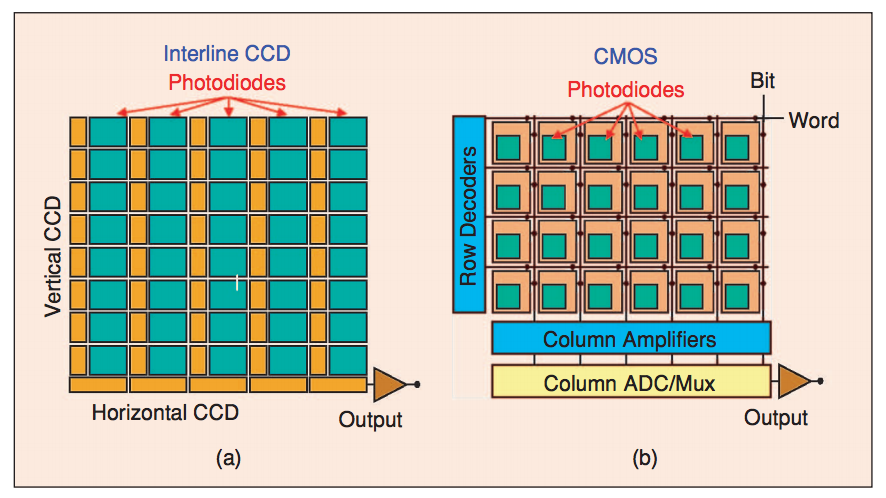
\includegraphics[scale=0.30]{sensor_arrays}
            \caption[CCD and CMOS sensor arrays.]{CCD and CMOS sensor arrays. Reproduced from Gamel et al \cite{gamal2005cmos}.}
            \label{fig:image_pipeline}
        \end{figure}

        \begin{figure}[H]
            \centering
            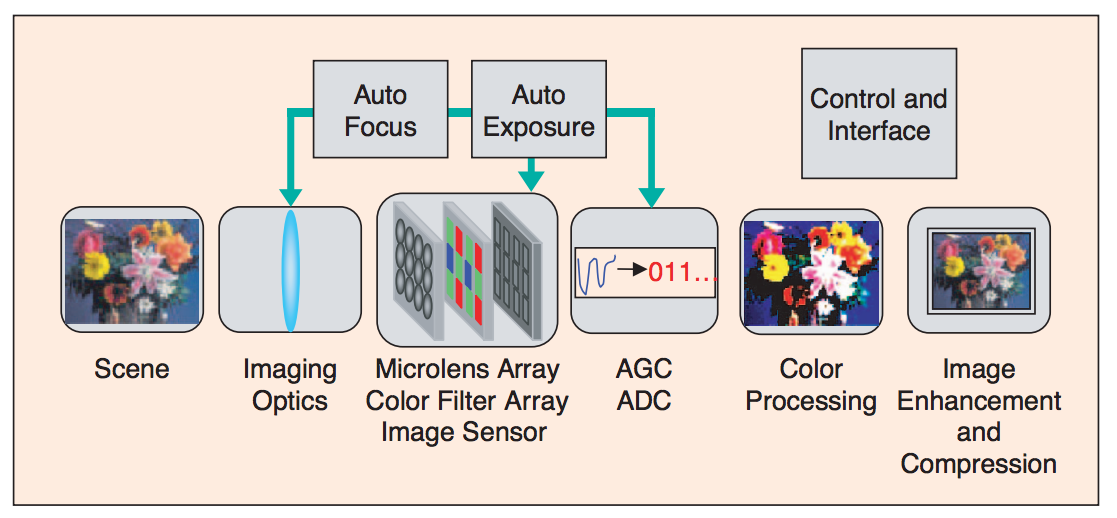
\includegraphics[scale=0.30]{imaging_pipeline}
            \caption[Overview of an imaging `pipeline'.]{Overview of an imaging `pipeline'. Reproduced from Gamel et al \cite{gamal2005cmos}.}
            \label{fig:image_pipeline}
        \end{figure}

        In a camera we have a focussing lens, followed by wavelength filters and then sensors. In many medical imagers 
        there is a collimator, so it is appropriate to consider a model where we have parallel streams of photons 
        hitting each sensor.

        \begin{figure}[H]
            \centering
            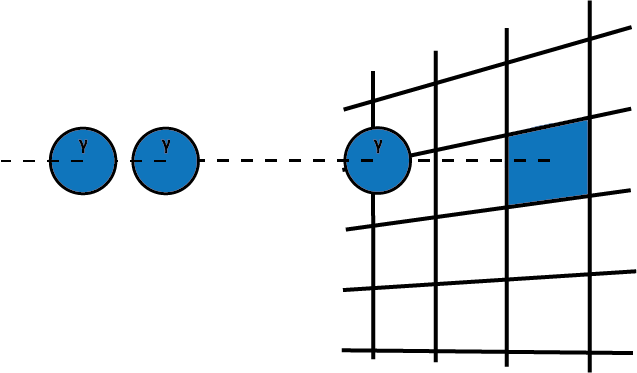
\includegraphics[scale=0.5]{photon_stream}
            \caption{Parallel stream of photons incident on one sensor in a sensor array.}
            \label{fig:photon_stream}
        \end{figure}

        We consider that a stream of photons, will be hitting some photodiode (the 
        part of a sensor that generates a current upon absorbtion of a photon), causing charge to collect on a connected 
        capacitor, which will increase linearly with respect to time at a rate proportional to the rate of photons 
        incident on the photoreceptor (the photocurrent), until it hits some maximum value. \cite{gamal2005cmos}

        \begin{figure}[H]
            \centering

                \begin{tikzpicture}
                    \begin{axis}[
                        name = plot2,
                        axis lines = left,
                        xtick={0,1},
                        xticklabels={$\ $,$t_{\text{exposure}}$},
                        ytick={0,1},
                        yticklabels={$\ $,$Q_{\text{max}}$},
                        xlabel = $t$ (time),
                        ylabel = $Q$ (charge),
                        legend pos=outer north east,
                        xmin=0,
                        ymin=0,
                        xmax=1.1,
                        ymax=1.1
                    ]
                        \draw[dotted] (axis cs:0,1) -- (axis cs:1.2,1);
                        \draw[dotted] (axis cs:1,0) -- (axis cs:1,1.2);
                        \addplot[domain=0:0.75, samples = 5, red] {4 * x/3};
                        \addlegendentry{`High light'};
                        \addplot[domain=0:1, samples = 5, blue] {x/2};     %N.b. filthy haxx to get legend to show 1 red, 1 blue instead of 2 red
                        \addlegendentry{`Low light'};
                        \addplot[domain=0.75:1, samples = 5, red] {1};
                    \end{axis}

                \end{tikzpicture}

            \caption{The charge held on a capacitor is linear with respect time, until it hits some maximum \cite{gamal2005cmos}.}
            \label{fig:linear_charge_wrt_photon_rate}
        \end{figure}


    \section{Quantum noise} \label{sec:quantum_noise}
        \textit{Quantum noise}, \textit{Photon noise} or \textit{Poisson noise} can be thought of as a uncertainty 
        associated with the measurement of light, due to the quantised nature of electromagnetic waves and the 
        independence of photon detections \cite{hasinoff2014photon}. More mathematically suppose we have some 
        noiseless image $I(x,y)$, then we define an image corrupted by photon noise $\tilde{I}$ by

        \begin{align}
            \tilde{I}(x,y) \sim \text{Poisson}(I(x,y)).
        \end{align}

        So we have

        \begin{align}
            \Pr(\tilde{I}(x,y) = k) & = 
                \begin{cases}
                    e^{-I(x,y)} \frac{I(x,y)^k}{k!} & 0 \leq k              \label{eq:image_poisson} \\
                    0 & \text{otherwise}
                \end{cases} \\
            \bb{E}\left[ \tilde{I}(x,y) \right] & = I(x,y) \\
            \var\left[ \tilde{I}(x,y) \right] & = I(x,y).                 
        \end{align}

        It is appropriate to consider a procvess such as the one in Figure \ref{fig:photon_stream} as a Poisson process, where 
        each event is a photon hitting the photoreceptor. Suppose the exposure time to the sensor is 
        $t_{\text{exposure}}$, the average rate of events is $\phi$ and that $N(t)$ is the number of events that 
        occur in the interval $[0,t]$, then we have $N(t) \sim \text{Poisson}(\phi t)$ \cite{ross2002probability}. 
        Thus we have $N(t_{\text{exposure}}) \sim \text{Poisson}(\phi t_{\text{exposure}})$. From figure 
        \ref{fig:linear_charge_wrt_photon_rate} we can justifiably say that if $\phi$ is the flux (rate) of 
        photons hitting sensor at index $(x,y)$ in the array, then $I(x,y) \propto N(t_{\text{exposure}})$.
        
        The model is easily and obviously extended to spatial images by including spectral bin indices 

        \begin{align}
            \tilde{I}(x,y,\lambda) \sim \text{Poisson}(I(x,y,\lambda)).
        \end{align}

        Because of the filters (shown in Figure \ref{fig:image_pipeline}) being spatially separated we can consider 
        each value in the datacube to be an independent random variable. This means that 

        \begin{align}
            (x,y,\lambda) \neq (x',y',\lambda') \Rightarrow 
                  \Pr(\tilde{I}(x,y,\lambda), \tilde{I}(x',y',\lambda')) = \Pr(\tilde{I}(x,y,\lambda)) \Pr(\tilde{I}(x',y',\lambda')).
        \end{align}

        However, in images the values are constrained to a finite range, typically we have that for each $x, y, 
        \lambda$ that $I(x,y,\lambda) \in \bb{N}_{256}$, but this however doesn't restrict the value of
        $\tilde{I}(x,y,\lambda)$ to $\bb{N}_{256}$. Let $\phi_{\text{crit}}$ be the rate which reaches charge 
        $Q_{\text{max}}$ at time $t_{\text{exposure}}$. By considering Figure \ref{fig:linear_charge_wrt_photon_rate} 
        we see that the charge becomes \textit{saturated} at the upper limit, that is for $\phi > \phi_{\text{crit}}$
        (from Figure \ref{fig:linear_charge_wrt_photon_rate}) we achieve $Q_max$, but for $\phi < \phi_{\text{crit}}$ 
        we don't achieve this before $t_{\text{exposure}}$. Thus for any $\phi > \phi_{\text{crit}}$ the maximum 
        value is recorded in the image values. To deal with this it makes sense to define a 
        \textit{Saturated Poisson} distribution. So we say $X \sim \text{SPoisson}(\mu, n)$ if 

        \begin{align}
            \Pr(X = k) & = 
                \begin{cases}
                    e^{\mu} \frac{\mu^k}{k!} & 0 \leq k < n-1 \\
                    \sum\limits_{i=n-1}^\infty e^{\mu} \frac{\mu^i}{i!} & k = n-1 \\
                    0 & \text{otherwise}.
                \end{cases} 
        \end{align}

        \begin{figure}[H]
            \centering 
            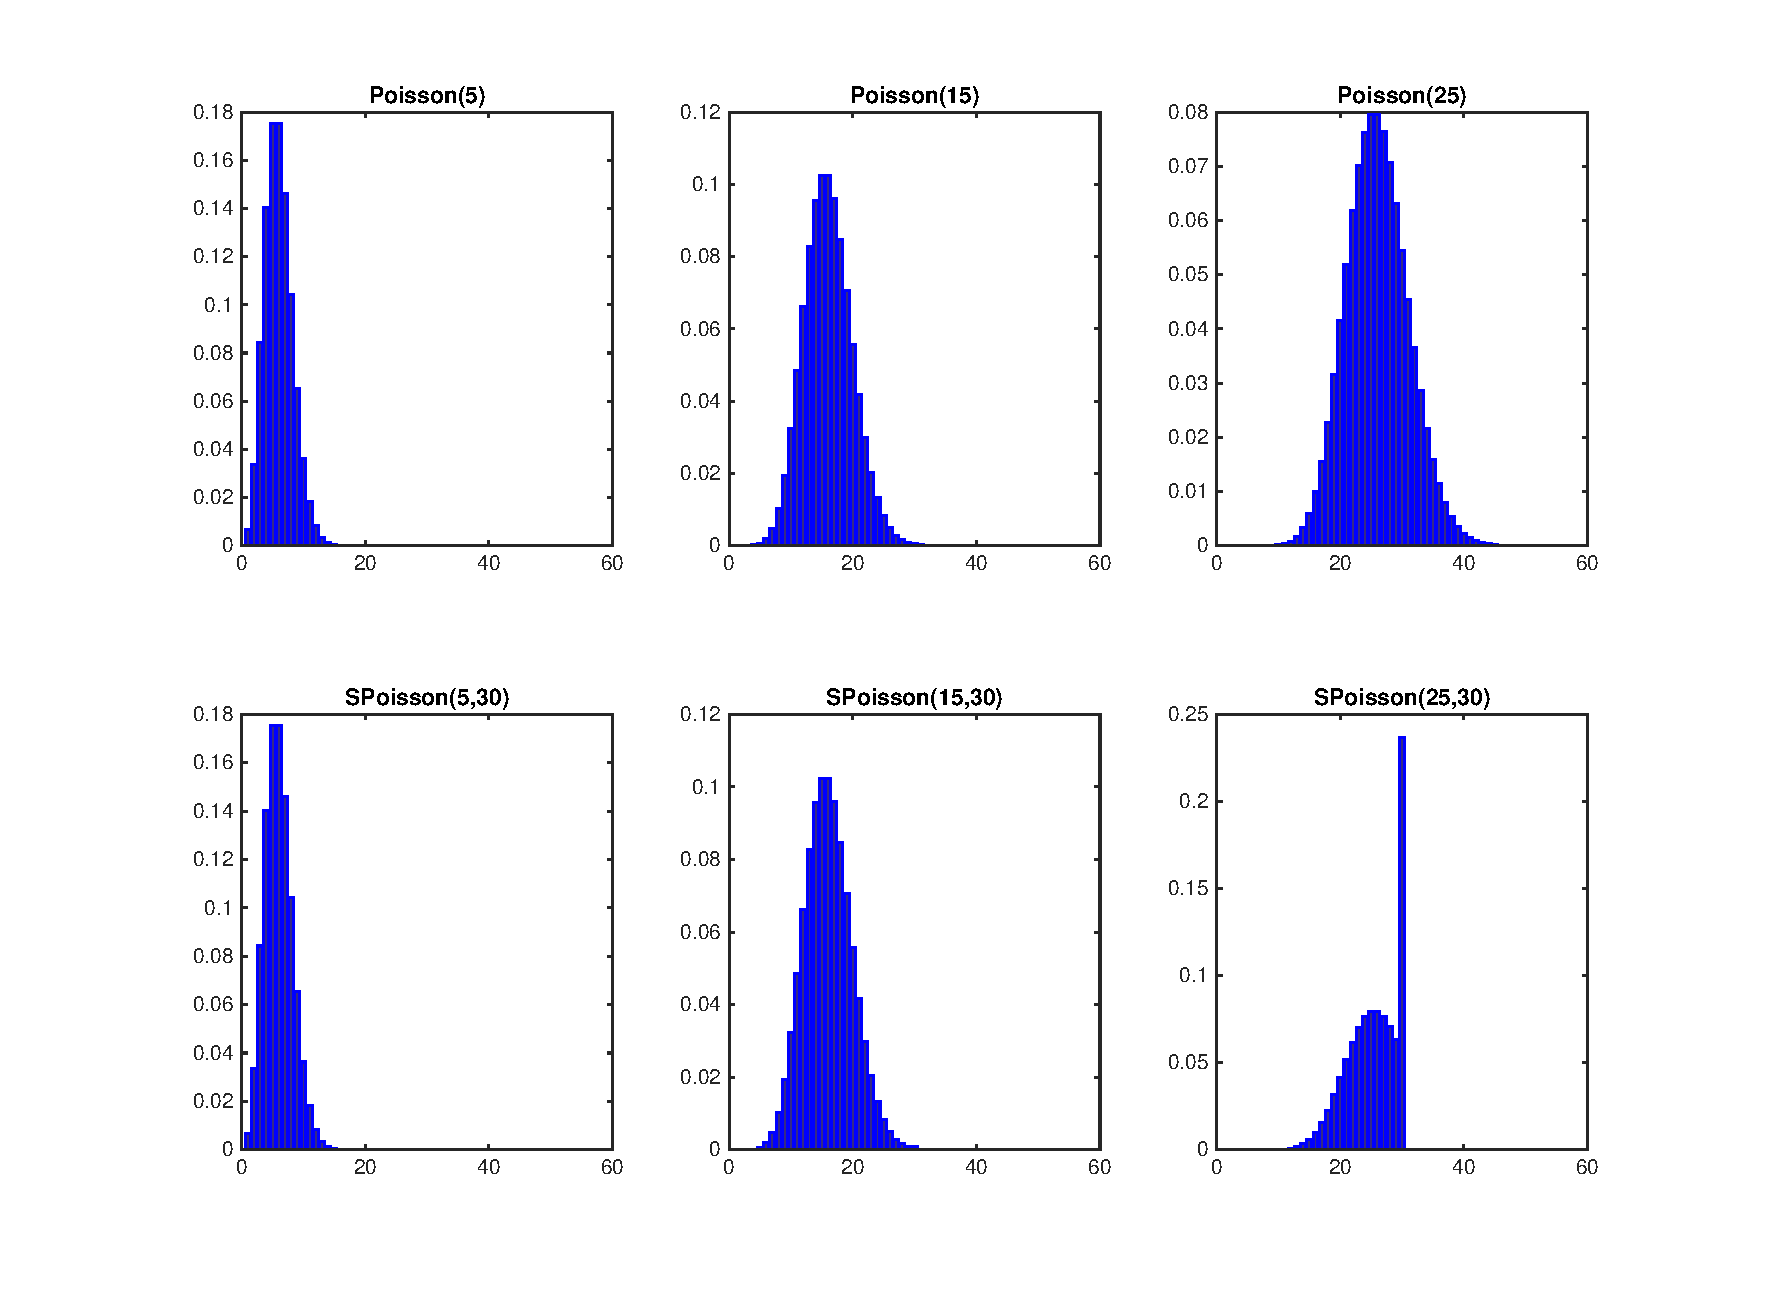
\includegraphics[scale=0.5]{poisson_distributions}
            \caption[Example of Poisson($\mu$) and SPoisson($\mu$, 30) distributions.]{Example of Poisson($\mu$) and SPoisson($\mu$, 30) distributions, for $\mu = 5,15,25$.}
        \end{figure}

    \section{Additive White Gaussian Noise}
        A more general noise model that should also be considered is \textit{additive white Gaussian Noise}. We will 
        `saturate' values with similar reasoning to section \ref{sec:quantum_noise}. The general model will add a 
        value sampled from a Gaussian distribution with some constant power. That is if we have a `true spectral image' 
        $I$, then the image corrupted by noise is:

        \begin{align}
            \tilde{I}(x,y,\lambda) = I(x,y,\lambda) + X_{ij\lambda}
        \end{align}

        where for each $i, j, \lambda$ we let $X_{ij\lambda} \sim N(0, \sigma^2)$. The noise is parametrised by 
        $\sigma$ and $\bb{E}[X_{ij\lambda}] = \sigma^2$ is the \textit{power} of the noise.








%%%%%%%%%%%%%%%%%%%%%%%%%%%%%%%%%%%%%%%%%%%%%%%%%%%%%%%%%%%%%%%%%%%%%%%%%%%%%%%%%%%%%%%%%%%%%%%%%%%%%%%%%%%%%%%%%%%%%%%%
% code listing for training

\cleardoublepage
\chapter{Code for training a decision forest} \label{app:train_tree}
    
    \begin{lstlisting}[caption={The implementation code for tree generation.}, label={lst:actualGenerateTree}]
private static TreeNode generateTree(
  TrainingSequence trainingSequence, 
  WeakLearner weakLearner, 
  int depth, 
  int randomnessParameter, 
  double informationGainCutoff) 
    throws MalformedProbabilityDistributionException {

  // Check for the training sequence being 0 in size, that 
  // should never happen
  if (trainingSequence.size() == 0) {
    throw new IllegalArgumentException(
      "Can't generate a tree from an empty sequence.");
  }
  
  // If the depth is zero or there is only one sample in 
  // the training sequences, then we need to create a leaf 
  // node, take the class as the majority vote from the 
  // training sequence.
  if (depth <= 0 || trainingSequence.size() == 1) {
    return new TreeNode(trainingSequence);
  }
  
  // Give the weak learner the training sequence as a hint
  // for what subspace of the split parameter space it 
  // should search
  weakLearner.giveHint(trainingSequence);
  
  // We will generate split paramters, and we will keep 
  // track of the best split. Initialise best information 
  // gain to -1.0 so we have a check that it was explicitly 
  // set at least once in the loop 
  double bestInformationGain = -1.0;
  TrainingSequence bestLeftSplit = null;
  TrainingSequence bestRightSplit = null;
  SplitParameters bestSplitParameters = null;
  int dataDimension = trainingSequence.trainingSequence.
      get(0).instance.getDimension();
  
  // Try "randomnessParameter" number of random split 
  // parameters
  for (int i = 0; i < randomnessParameter; i++) {
    SplitParameters splitParameters = 
      weakLearner.generateRandomSplitParameters(
        dataDimension);
    List<TrainingSample> leftList = new ArrayList<>();
    List<TrainingSample> rightList = new ArrayList<>();
    
    // Split the training sequence into a left and right split
    for (TrainingSample sample : 
        trainingSequence.trainingSequence) {

      if (weakLearner.split(splitParameters, sample.instance) 
            == Direction.LEFT) {
        leftList.add(sample);
      } else {
        rightList.add(sample);
      }
    }
    
    // See what information gain this leads to
    TrainingSequence leftSplit = new TrainingSequence(
      leftList, trainingSequence.classes);
    TrainingSequence rightSplit = new TrainingSequence(
      rightList, trainingSequence.classes);
    double informationGain = 
      TrainingSequence.informationGain(leftSplit, rightSplit);
    
    // If its the best information gain found so far, 
    // remember it!
    if (informationGain > bestInformationGain) {
      bestInformationGain = informationGain;
      bestLeftSplit = leftSplit;
      bestRightSplit = rightSplit;
      bestSplitParameters = splitParameters;
    }
  }
  
  // We make a greedy choice using the best split that we 
  // found, and recursively build our child nodes.
  // N.B. If the split doesn't gain enough information, then 
  // just try again, (so we've used up "one depth").
  // N.B.B. informationGainCutoff >= 0.0, and if one of the 
  // sequences is empty, then there is and information gain of 
  // 0.0, hence if one of the sequences is empty we don't EVER 
  // pass the information gain cutoff. Hence any split that 
  // actually causes a recursion will have two non empty 
  // subsequences.
  TreeNode node = null;
  if (bestInformationGain <= informationGainCutoff) {
    node = generateTree(trainingSequence, weakLearner, depth-1, 
        randomnessParameter, informationGainCutoff);
  } else {
    TreeNode leftChild = 
      generateTree(bestLeftSplit, weakLearner, depth-1, 
        randomnessParameter,informationGainCutoff);
    TreeNode rightChild = 
      generateTree(bestRightSplit, weakLearner, depth-1, 
        randomnessParameter, informationGainCutoff);
    node = 
      new TreeNode(trainingSequence, leftChild, rightChild, 
        bestSplitParameters, bestInformationGain);
  }
  
  // We have trained a tree! Return it
  return node;
}
    \end{lstlisting}


    \begin{lstlisting}[caption={The implementation code for training a decision forest.}, label={lst:actualTrainForest}]
public static DecisionForest trainDecisionForest(
    final TrainingSequence trainingSequence, 
    final WeakLearner weakLearner, 
    final int maxTrees, 
    final int maxDepth, 
    final int randomnessParameter,
    final double informationGainCutoff, 
    final boolean normaliseInstances, 
    final boolean bagging) 
    throws MalformedForestException, 
      MalformedProbabilityDistributionException, 
      InterruptedException {
  
  // If we are given nonsensical input, throw an exception
  if (trainingSequence == null || trainingSequence.size() == 0 
    || trainingSequence.classes.size() == 0) {
    throw new IllegalArgumentException("We need a non-empty, "
        + "non-null training sequence to train a tree.");
  } else if (weakLearner == null) {
    throw new IllegalArgumentException("We need a non-null "
        + "weak learner to be able to train a tree.");
  } else if (maxTrees <= 0) {
    throw new IllegalArgumentException("A non-positive "
        + "number of trees doesn't make sense for a forest.");
  } else if (maxDepth <= 0) {
    throw new IllegalArgumentException("A non-negative depth "
        + "doesn't make sense for a tree. A tree consisting "
        + "of a single node has depth 0. If we limit trees to "
        + "be just leaves then there is no decisions being " 
        + "made - the tree does nothing.");
  } else if (randomnessParameter <= 0) {
    throw new IllegalArgumentException("We need a positive "
        + "randomness parameter, it doens't make sense to " 
        + "have a negative quantity.");
  } else if (informationGainCutoff < 0.0) {
    throw new IllegalArgumentException("Information gain is "
      + "a strictly non-negative value, so must have a cutoff "
      + "of more than or equal to zero.");
  }
  
  // Normalise the training sequence if we want that
  // Remember the reference value (power)
  double normalisationReference = 0.0;
  if (normaliseInstances) {
    normalisationReference = trainingSequence.normalise();
  }
  
  // Create a DecisionForest instance
  DecisionForest forest = new DecisionForest();
  forest.setDataDimension(trainingSequence.trainingSequence.
    get(0).instance.getDimension());
  forest.setClasses(trainingSequence.classes);
  forest.setWeakLearnerType(weakLearner.getWeakLearnerType());

  // Use a new thread to build each tree
  final Set<DecisionForest.TreeNode> rootNodes = 
    new HashSet<>();
  Set<Thread> workers = new HashSet<>(); 
  for (int i = 0; i < maxTrees; i++) {
    
    // Train the new tree in its own thread
    Thread thread = new Thread() {
      public void run() {
        // Perform bagging of the training sequence if we want
        TrainingSequence ts = trainingSequence.bag();
        if (bagging) {
          ts = trainingSequence.bag();
        }
        
        // Generate the tree node
        TreeNode node = generateTree(ts, weakLearner, maxDepth, 
            randomnessParameter, informationGainCutoff);
        node.compact();
        synchronized(rootNodes) {
          rootNodes.add(node);
          System.out.println("Tree number " + rootNodes.size() 
            + " trained.");
        }
      } 
    };
    thread.start();
    workers.add(thread);
  }
  
  // Wait for the threads to finish
  for (Thread thread : workers) {
    thread.join();
  }
  
  // Add the root nodes to the forest structure
  forest.setRootNodes(rootNodes);
  
  // Add normalisation variables to the forest structure
  forest.setNormalisedClassification(normaliseInstances);
  forest.setNormalisationReference(normalisationReference);
  
  // Return the constructed forest
  return forest;
}
      \end{lstlisting}











%%%%%%%%%%%%%%%%%%%%%%%%%%%%%%%%%%%%%%%%%%%%%%%%%%%%%%%%%%%%%%%%%%%%%%%%%%%%%%%%%%%%%%%%%%%%%%%%%%%%%%%%%%%%%%%%%%%%%%%%
% code listing for classification

\cleardoublepage
\chapter{Code for classifying using a decision forest} \label{app:classify_tree}

    \begin{lstlisting}[caption={The implementation code for tree traversal.}, label={lst:actualTraverseTree}]
private ProbabilityDistribution traverseTree(
  WeakLearner splitter, 
  Instance instance) 
    throws MalformedForestException {

  try {
    // Use the split function to traverse the tree until we 
    // hit a root node
    TreeNode currentNode = this;
    while (!currentNode.isLeafNode()) {
      Direction splitDirection = 
        splitter.split(currentNode.splitParams, instance);

      if (splitDirection == Direction.LEFT) {
        currentNode = currentNode.leftChild;
      } else {
        currentNode = currentNode.rightChild;
      }
    }
    
    // Return the class associated with the root node
    return currentNode.probabilityDistribution;
    
  } catch (NullPointerException ex) {
    // If we get a null pointer, then we must have a 
    // malformed tree
    throw new MalformedForestException("Failed traversing a "
      + "tree due to null pointer exception.");
  }
}
    \end{lstlisting}

    \begin{lstlisting}[caption={The implementation code for classification using a decision forest.}, label={lst:actualTraverseTree}]
public ProbabilityDistribution classify(
  final Instance instance) {
  
  // Create a splitter depending on our weak learner type
  final WeakLearner splitter;
  switch (weakLearnerType) {
    case ONE_DIMENSIONAL_LINEAR:
      splitter = new OneDimensionalLinearWeakLearner();
      break;
    default:
      throw new MalformedForestException("No weak learner for "
        + "the type given, unable to classify.");
  }
  
  // If we are using normalised labeling, then normalise
  if (normalisedClassification) {
    instance.normalise(normalisationReference);
  }
  
  // Define a wrapper for the accumulator distribution
  // We use this as a closure in the threads, so we get past 
  // the restriction of only using final variables in threads
  final class AccumulatorDistributionWrapper {
    ProbabilityDistribution accDistr;
    int distributionsSummed;
  }
  
  // Define the accumulator distribution we use
  final AccumulatorDistributionWrapper wrapper = 
    new AccumulatorDistributionWrapper();
  
  // Compute the trees votes in parallel, and then add them 
  // together in an accumulating probability distribution
  Set<Thread> threads = new HashSet<>();
  for (final TreeNode node : rootNodes) {
    
    // Run the traversal in a new thread
    Thread thread = new Thread() {
      public void run() {
      // Traverse to the leaf distribution, then add it to the 
      // accumulating
      ProbabilityDistribution leafDistr = 
        node.traverseTree(splitter, instance);

        synchronized(wrapper) {
          if (wrapper.distributionsSummed == 0) {
            wrapper.accDistr = leafDistr;
          }
          else {
            wrapper.accDistr.addRunningTotal(
              leafDistr, wrapper.distributionsSummed+1);
          }
          wrapper.distributionsSummed++;
        }
      }
    };
    threads.add(thread);
    
  }
  
  // Wait for the threads to finish
  for (Thread thread : threads) {
    thread.join();
  }
  
  // Return the probability distribution
  return wrapper.accDistr;
}
    \end{lstlisting}









%%%%%%%%%%%%%%%%%%%%%%%%%%%%%%%%%%%%%%%%%%%%%%%%%%%%%%%%%%%%%%%%%%%%%%%%%%%%%%%%%%%%%%%%%%%%%%%%%%%%%%%%%%%%%%%%%%%%%%%
project proposal

\cleardoublepage
\chapter{Project Proposal}

\vfil

\centerline{\Large Computer Science Project Proposal}
\vspace{0.4in}
\centerline{\Large Spectral Image Analysis for Medical Imaging}
\vspace{0.4in}
\centerline{\large M. Painter, Churchill College}
\vspace{0.3in}
\centerline{\large Originator: Dr. Pietro Lio'}
\vspace{0.3in}
\centerline{\large \date{\today}}

%\vfil


\noindent
{\bf Project Supervisor:} Dr Pietro Lio', Dr Gianluca Ascolani
\vspace{0.2in}

\noindent
{\bf Director of Studies:} Dr John Fawcett
\vspace{0.2in}
\noindent
 
\noindent
{\bf Project Overseers:} Prof John Daugman \& Dr David Greaves


% Main document
% ------------------------------------------------------------------------------

\section*{Introduction and Description of the Work}
The core idea of the project is to use spectral algorithms and machine learning 
to analyse biomedical images. I will explore the use of multiple learning 
techniques (namely Random Decision Forests and Neural Networks) and compare them 
via a number of metrics, described later. \\

The aim of the project will be to build a classifier that is capable of handling 
a wide variety of noisy medical images. Different types of medical images 
will present different challenges such as contrast between tissues and amount 
and type of noise. It will classify images per pixel into classes (dependent on 
the image), using the spectral analysis. \\

During the implementation I will start by implementing something for a toy 
problem, by which I mean an artificially produced, noiseless image. From this 
solution I will move onto solving the same problem with the introduction of 
artificial noise, at which point I will explore the use of de-noising 
techniques to improve the accuracy of the classifier. Finally after this I will 
move onto an implementation for real images. \\

For the real images I will use MRI images from Zhongzhao Teng from the Department 
of Radiology, Engineering, which include fatty tissues from patients with 
atherosclerosis (the build up of fatty tissues in arteries). In this case I can 
train the classifier to recognise regions of calcium, lipids, haemorragic tissue, 
and mixtures of these. \\

To demonstrate the versatility of the tool I will also use another set of images 
obtained in a completely different way, so will present a different set of 
challenges including the nature of noise in the image. The images are from Siri 
Luthman of the BSS group in the Department of Physics, and are obtained using a 
hyper-spectral camera with 72 spectral bins. The images use contrast agents with 
various spectral profiles, each of which has a negative binding response or 
neutral binding response for cancerous cells. By `negative binding response' I 
mean that the contrast agent binds to only non-cancerous cells, and `neutral' 
means that it binds to both cancerous and non-cancerous cells. Here the classes 
will be cancer cells, non-cancerous cell, and a mixture of both.







% The core of the project will perform spectral analysis of images and use this 
% for classifying images.

% -Explore spectral analysis of noisy images
% -Will compare different algorithms
% -MRI is about art....
% -Siri has provided images and I will do spectral analysis on it
% -Why do different image sets?
% - Diff types of noise - one is MRI
% - Medical images give many different challenges, diff data and diff ammount of noise, different contrasts between tissues.
% - Represent different challenges
% - See if can be adaptive enough to solve challenges of both images
% - Using specral methods - fourier transform and wavelets
%             - machine learning like random forests
% - different types of image with different 

% - de-noise and classify
%         - teng slideshow
%         - siri slideshow
%             -say what they are doing

% - neural networks and deep learning 
% - scrap GPU
% extension use machine learning and deep learning


% - give them something that describes the images for them.

% take some stuff from books and slides and not just siri
%         - not too much siri, physics and cl `speak diff languages'

% ---- What is the point?

% - don't talk about extension in intro, it has own section

% -diff noise from diff types of measurement and different techniques

% - meanwhile i will use to use these methods



% -start with an easy benchmark -> red circle on a black background
%                               -> standard benchmarks
%                               -> then add noise
%                               -> then move to medical images

%                               -> see anything interesting put into file.
%                               -> Pietro send lots of material, when see something interesting and then ask for the code if it's interesting.





% The core project is to implement a classifier of spectral images using a 
% machine learning algorithm, more specifically for use with medical imaging. I 
% will look at using different machine learning algorithms during my research 
% phase, and will implement at least one of these. \\

% In many medical images only some regions contain the cells/tissues that we are 
% interested in, so it would be useful to have a tool to indicate which regions 
% are of interest when teaching the machine. \\

% From some initial reading it appears that I may wish to use the Random 
% Forests algorithm, but this is something that I will want to look into further 
% at the beginning of my project. \\

% The system will initially just classify images as ``X'' is present in the image. 
% And hopefully if time will be able to indicate the regions of the image where 
% ``X'' is present. \\

% There will be many `endmembers' that will contribute to each pixels spectrum 
% seen in any medical image and so it is useful to be able to classify what might 
% be contained in each pixel. As I will be classifying per pixel it may be 
% amenable to GPU programming (which I will leave as an extension).



% ------------------------------------------------------------------------------

\section*{Starting Point}

I will use Java for the implementation of my algorithms and use libraries 
provided for Java. I will also use OpenCV's machine learning library as a 
benchmark to test my implementations against. 



% ------------------------------------------------------------------------------

\section*{Resources Required}

I will use my own computer to code on as I am more comfortable with it than the 
MCS machines. \\

I will also need example (spectral) image sets to be used in training and 
testing. I have kindly been provided with some MR images by Zhongzhao Teng of 
the Department of Ragiology and some hyperspectral images from Siri Luthman of 
the BSS group in the Department of Physics, as mentioned in the introduction.



% ------------------------------------------------------------------------------

\section*{Backup Plan}

I will be using a git repository for my project, which will be a private 
repository on GitHub. I will have two branches (at least, more if necessary) one 
`master' for completed features and one `in progress'. The in progress branch 
will be to push regularly any unfinished/in progress work onto so that my work 
is always backed up, and I don't loose any work in progress. \\

The local folder will also be in my Google Drive folder and so will be 
automatically synced to the Google servers, and I also have a time machine 
set up, which will take backups of the whole file system every hour.




% ------------------------------------------------------------------------------

\section*{Work to be done}

I can break down the project into the following stages:

\begin{enumerate}

\item 
Implement the infrastructure (data structures etc) and reading in of the raw
data.

\item 
Create a tool used to indicate areas of interest on the teaching data to be used 
with the training data.

\item 
Implement the main machine learning algorithm(s), and implement an out the 
box solution, initially to solve the `toy problem'. 

\item 
Extend the implementation to work for noisy images and then real images.

\end{enumerate}



% ------------------------------------------------------------------------------

\section*{Success Criterion for the Main Result}

I will use an `out the box' solution (such as OpenCV's machine learning 
libraries) as a benchmark to compare my implementation(s) against. I 
will provide each machine learning algorithm with the same inputs for training 
and the same inputs for testing and will use the following metrics to compare 
the performance of the systems and which has `learnt' better:
\begin{itemize}
    \item Overall run time (of classifying a single image);
    \item Accuracy of classifier (percentage images correctly identified).
\end{itemize}



% ------------------------------------------------------------------------------

\section*{Possible Extensions}

\begin{itemize}

    \item
    {\em Image Segmentation.}

    It would be useful to be able to segment the images given into separate 
    regions of interest. (For example if we want to classify an image with 
    cancer cells present, we indicate the regions containing cancerous cells).
    This is opposed to just returning the output per pixel, and would provide 
    a more useful output for users.

    \item 
    {\em Dimensionality Reduction.}

    If I finish the core of my project then one of the additional tasks that I 
    could look at would be to implement a data reduction (learning) algorithm. 
    In a spectral image with a high number of spectral bands it would be useful 
    to identify which spectral bands are important to the classification and 
    which are not. \\

    This problem more generally is called ``dimensionality reduction'' as we are 
    looking to reduce the dimension of data input to the algorithm.

\end{itemize}



% ------------------------------------------------------------------------------
% Put the timetable on a separate page so that we can print it out
\clearpage
\section*{Timetable: Workplan and Milestones to be achieved.}

% - - - - - 
{\bf Michaelmas weeks 3--4 (26th Oct to 4th Nov)} 

In preparation for the main implementation I will read about many machine 
learning algorithms. For example I will use the book ``Decision Forests for 
Computer Vision and Medical Image Analysis'' to learn about Random Forests. I 
will similarly research about Neural networks, and I will also research some 
other forms of learning algorithm. \\

{\em Deliverables:} 
\begin{itemize} 
    \item 
    A small description/overview of random forests and how they work, and a 
    similar description for any other learning algorithms researched. This 
    should be written up in \LaTeX\ for easy embedding into the preparation 
    chapter of the dissertation.
\end{itemize}

{\em Milestones:}
\begin{itemize}
    \item 
    Preparation reading completed, so that I am sufficiently able to implement 
    the learning algorithm(s) and handed in description of reading to project 
    supervisor for review - 4th Nov.
\end{itemize}



% - - - - - 
{\bf Michaelmas weeks 5--6 (5th Nov to 18th Nov)} 

I will spend this block familiarising myself with any technologies that I will 
possibly use. This will include the OpenCV library. I will also 
design a simple UI that will be used for the supervised learning. I will also 
familiarise myself with OpenCL and GPU programming. \\

{\em Deliverables:} 
\begin{itemize} 
    \item 
    A sketch of the UI for the tool which will be used for the supervised 
    learning.
    \item 
    A small overview of what OpenCV, GPU programming (or other technology(s) I 
    have looked at), and a description of why/where they will be useful. This 
    should again be written up in \LaTeX\ for easy embedding into the 
    preparation chapter of the dissertation.
\end{itemize}

{\em Milestones:}
\begin{itemize}
    \item 
    Handed in the UI design to supervisor for review - 9th Nov
    \item 
    Handed in the description of familiarisation of technologies to supervisor 
    for review - 18th Nov.
    \item 
    Demonstrated any small programs written for familiarisation to supervisor - 
    18th Nov.
\end{itemize}




% - - - - - 
{\bf Michaelmas weeks 7--8 (19th Nov to 2nd Dec)} 

{\em Implementation block 1}. Implement the infrastructure that will be used for 
the project. This will include loading the raw data into the appropriate data 
structures and do so efficiently as possible. \\

{\em Deliverables:} 
\begin{itemize} 
    \item 
    A bullet point list indicating what has been implemented during this block. 
    Written up in \LaTeX\ and to be used as a basis for the implementation 
    portion of the dissertation. To be handed in for review.
\end{itemize}

{\em Milestones:}
\begin{itemize}
    \item 
    Have the framework that I will use completed, including unit tests, and 
    demonstrate the tests to supervisor to check that this has been done - 2nd 
    Dec.
\end{itemize}




% - - - - - 
{\bf Christmas vacation weeks 1--2 (3rd Dec - 16th Dec)} 

I will be on holiday during this period and so I will work on little bits 
when I can, this may be catching up on any work that I got behind on in 
Michaelmas term (effectively making this a `slack' block), and I will begin 
some work on the next block if up to date. \\






% - - - - - 
{\bf Christmas vacation weeks 3--4 (17th Dec - 30th Dec)} 

{\em Implementation block 2}. Write the tool that will be used to indicate 
which images (or image regions) belong to a given class to be used for the 
supervised learning. \\

{\em Deliverables:} 
\begin{itemize} 
    \item 
    A bullet point list indicating what has been implemented during this block. 
    Written up in \LaTeX\ and to be used as a basis for the implementation 
    portion of the dissertation.
\end{itemize}

{\em Milestones:}
\begin{itemize}
    \item 
    Sent the completed tool to my supervisor as proof of completion. (As it is 
    the vacation I will not be in Cambridge and so will not be able to 
    demonstrate in person). - 30th Dec
\end{itemize}




% - - - - - 
{\bf Christmas vacation weeks 5--6 (31st Dec - 13th Jan)} 

{\em Implementation block 3}. Implement the machine learning algorithm(s) 
chosen, and also write the `out of the box' solution using the OpenCV 
library. At this stage I will only aim to have  \\

If this block is delivered on time then I am close to having a completed 
project. I have purposely stacked more of the work in the holiday compared to 
term time, as I have other commitments in term than out of term, such as 
lectures and supervisions. \\

{\em Deliverables:} 
\begin{itemize} 
    \item 
    A bullet point list indicating what has been implemented during this block. 
    Written up in \LaTeX\ and to be used as a basis for the implementation 
    portion of the dissertation.
\end{itemize}

{\em Milestones:}
\begin{itemize}
    \item 
    Finished writing the machine learning algorithm, and demonstrated it 
    classifying some `toy images' to supervisor - 13th Jan. (I will be back in 
    Cambridge by this time).
\end{itemize}




% - - - - - 
{\bf Lent weeks 1--2 (14th Jan - 27th Jan)} 

The progress report needs to be given up by noon on the 29th Jan, and so should 
be written in this block. \\

This rest of this block will be kept free for `slack'. This slack should include 
incorporating any feedback from my supervisor. \\

If I am up to date and there is no additional feedback that needs to be resolved, 
then I will proceed to work a block ahead. This will give me an additional block 
at the end of lent to implement any extensions. \\

{\em Deliverables:} 
\begin{itemize} 
    \item 
    Progress report.
    \item 
    Item written in \LaTeX\ which begins with the supervisors comments/feedback 
    and ends with how that was incorporated into the system.
\end{itemize}

{\em Milestones:}
\begin{itemize}
    \item 
    Demonstration of any features added made to supervisor - 27th Jan
\end{itemize}




% - - - - - 
{\bf Lent weeks 3--4 (28th Jan - 10th Feb)} 

{\em Implementation block 4}. In this block I will finish implementing my 
solution, and extend my simple solution to a more complex one capable of 
handling `toy images' with artificial noise, and then real images. This will 
require implementing de-noising of the images. \\

Also after the progress report a small presentation needs to be prepared. I 
will use the beginning of this time block to do this. \\

{\em Deliverables:} 
\begin{itemize} 
    \item 
    A bullet point list indicating what has been implemented during this block. 
    Written up in \LaTeX\ and to be used as a basis for the implementation 
    portion of the dissertation.
\end{itemize}

{\em Milestones:}
\begin{itemize}
    \item 
    Hand in progress report (completed in the previous block) - 29th Jan.
    \item 
    Perform a small mock presentation/interview with supervisor - 3rd Feb.
    \item 
    Made progress presentation to overseer group - ~5th Feb.
    \item 
    Finished implementing any de-noising algorithms, and have a working solution 
    for real images, including a demonstration to supervisor - 10th Feb.
\end{itemize}




% - - - - - 
{\bf Lent weeks 5--6 (11th Feb - 24th Feb)} 

Evaluation of the system. This will require writing tests that will gather 
the quantitative data (run time and accuracy of classification) to be used in 
the comparison required to satisfy the success criteria.\\

I will generate graphs from data in this phase using MATLAB, so that I can 
decide if the data is useful or not. This will prevent me from realising that 
the data isn't good at too late a stage in the project and when there is not 
enough time to re-evaluate the system. This has the advantage that the graphs 
will be ready to be exported directly into the dissertation. \\

{\em Deliverables:} 
\begin{itemize} 
    \item 
    Table for any qualitative data evaluated and spreadsheet of quantitative 
    data, which must include values for accuracy of the system (in a specific 
    test case) and timings for how long classification takes (on my home 
    machine).
    \item 
    Generated meaningful graphs using MATLAB with data gathered from evaluation.
\end{itemize}

{\em Milestones:}
\begin{itemize}
    \item 
    Table/spreadsheet completed and filled out with all data required for a good 
    write up. Spreadsheet and graphs sent to supervisor for reviewing - 24th Feb.
\end{itemize}




% - - - - - 
{\bf Lent weeks 7--8 (25th Feb - 9th Mar)} 

I will use my last block of work in lent as another `slack' block for if I get 
behind on any work for any reason such as a high load of supervision work 
through the term. This should also be used to incorporate any final feedback 
from my supervisor. \\

If am up to date at this point  I will work on implementing some of the 
extension tasks outlined in this document.

{\em Milestones:}
\begin{itemize}
    \item 
    System complete, success criterion met and demonstrated these to supervisor 
    - 9th Mar.
\end{itemize}




% - - - - - 
{\bf Easter vacation weeks 1--2 (10th Mar - 23rd Mar)} 

Set up the dissertation document and write introduction and preparation 
chapters of the dissertation. \\

{\em Deliverables:} 
\begin{itemize} 
    \item 
    Introduction and preparation chapters of dissertation.
\end{itemize}

{\em Milestones}: 
\begin{itemize}
    \item 
    Completed first draft of introduction chapter and given to supervisor 
    - 17th Mar.
    \item 
    Completed first draft of preparation chapter and given to supervisor 
    - 23rd Mar.
\end{itemize}




% - - - - - 
{\bf Easter vacation weeks 3--4 (24th Mar - 6th Apr)} 

Write up the implementation and evaluation chapters of the dissertation. \\

{\em Deliverables:} 
\begin{itemize} 
    \item 
    Implementation and evaluation chapters of dissertation.
\end{itemize}

{\em Milestones:}
\begin{itemize}
    \item 
    Completed first draft of implementation chapter and given to supervisor 
    - 31st Mar.
    \item 
    Completed first draft of the evaluation chapter and given to supervisor 
    - 6th Apr.
\end{itemize}




% - - - - - 
{\bf Easter vacation weeks 5--6 (7th Apr - 20th Apr)} 

Complete dissertation by completing the conclusion section and any appendices. 
I will also re-iterate through dissertation see if anything can be improved. \\

{\em Deliverables:} 
\begin{itemize} 
    \item 
    Draft of complete dissertation.
    \item 
    2nd draft of complete dissertation.
\end{itemize}

{\em Milestones:}
\begin{itemize}
    \item 
    Full first draft of dissertation handed into supervisor for review - 11th 
    Apr.
    \item 
    Hand in second draft of completed dissertation to supervisor - 18th Apr.
\end{itemize}


% - - - - - 
{\bf Easter term weeks 1--2 (21st Apr - 5th May)}  

Final `slack' block for the dissertation. If the dissertation is completed then 
I will proof read multiple times. I would like to have the dissertation 
`finished' by now to focus on revision for the exam and on learning any of the 
Easter term courses. \\

{\em Milestones:}
\begin{itemize}
    \item 
    System complete and success criterion met - 5th May.
\end{itemize}



% - - - - - 
{\bf Easter term week 3 (6th May - 13th May)} 

Final proof read and then an early submission so that I can focus on exam 
revision for the remainder of the term. \\

{\em Deliverables:} 
\begin{itemize} 
    \item 
    Dissertation.
\end{itemize}

{\em Milestones:}
\begin{itemize}
    \item 
    Hand in dissertation on time. (Project finished). - 13th May.
\end{itemize}













%%%%%%%%%%%%%%%%%%%%%%%%%%%%%%%%%%%%%%%%%%%%%%%%%%%%%%%%%%%%%%%%%%%%%%%%%%%%%%%%%%%%%%%%%%%%%%%%%%%%%%%%%%%%%%%%%%%%%%%%
% the glossary

\cleardoublepage
\chapter{Glossary}
\glsaddall
\printglossaries

\end{document}
